% Start preamble
\documentclass[12pt,a4paper]{article}
\usepackage{geometry}
 \geometry{
 a4paper,
 total={170mm,257mm},
 left=20mm,
 top=20mm,
 }
\usepackage[utf8]{inputenc}
\usepackage[T1]{fontenc}
\usepackage[pdftex]{graphicx}
\graphicspath{{./}}
\usepackage{enumitem}
\usepackage{pdfpages}
\usepackage{hyperref}
\usepackage{tikz}
\usepackage{attachfile}
\usepackage{epstopdf}
\usepackage{array}
%\usepackage[table]{xcolor,colorbl}
\setlength{\textwidth}{16cm}
\setlength{\oddsidemargin}{-0.5cm}
\setlength{\evensidemargin}{-0.5cm}
%\setlenght{\headsep}{0cm}
\setlength\parindent{0pt}
%\setlength{\extrarowheight}{3pt}
\usepackage{listings}
%\usepackage{xcolor}

 %%%%%%%%%%%%%%%%%%%%%%%%%%%%%%%%%%%%%%%%%%%%%%%%%%%%%%%%%%%%%%%%%%%%%%%%%%%%%%%% 
%%% ~ Arduino Language - Arduino IDE Colors ~                                  %%%
%%%                                                                            %%%
%%% Kyle Rocha-Brownell | 10/2/2017 | No Licence                               %%%
%%% -------------------------------------------------------------------------- %%%
%%%                                                                            %%%
%%% Place this file in your working directory (next to the latex file you're   %%%
%%% working on).  To add it to your project, place:                            %%%
%%%     %%%%%%%%%%%%%%%%%%%%%%%%%%%%%%%%%%%%%%%%%%%%%%%%%%%%%%%%%%%%%%%%%%%%%%%%%%%%%%%% 
%%% ~ Arduino Language - Arduino IDE Colors ~                                  %%%
%%%                                                                            %%%
%%% Kyle Rocha-Brownell | 10/2/2017 | No Licence                               %%%
%%% -------------------------------------------------------------------------- %%%
%%%                                                                            %%%
%%% Place this file in your working directory (next to the latex file you're   %%%
%%% working on).  To add it to your project, place:                            %%%
%%%     %%%%%%%%%%%%%%%%%%%%%%%%%%%%%%%%%%%%%%%%%%%%%%%%%%%%%%%%%%%%%%%%%%%%%%%%%%%%%%%% 
%%% ~ Arduino Language - Arduino IDE Colors ~                                  %%%
%%%                                                                            %%%
%%% Kyle Rocha-Brownell | 10/2/2017 | No Licence                               %%%
%%% -------------------------------------------------------------------------- %%%
%%%                                                                            %%%
%%% Place this file in your working directory (next to the latex file you're   %%%
%%% working on).  To add it to your project, place:                            %%%
%%%    \input{arduinoLanguage.tex}                                             %%%
%%% somewhere before \begin{document} in your latex file.                      %%%
%%%                                                                            %%%
%%% In your document, place your arduino code between:                         %%%
%%%   \begin{lstlisting}[language=Arduino]                                     %%%
%%% and:                                                                       %%%
%%%   \end{lstlisting}                                                         %%%
%%%                                                                            %%%
%%% Or create your own style to add non-built-in functions and variables.      %%%
%%%                                                                            %%%
 %%%%%%%%%%%%%%%%%%%%%%%%%%%%%%%%%%%%%%%%%%%%%%%%%%%%%%%%%%%%%%%%%%%%%%%%%%%%%%%% 

\usepackage{color}
\usepackage{listings}    
\usepackage{courier}

%%% Define Custom IDE Colors %%%
\definecolor{arduinoGreen}    {rgb} {0.17, 0.43, 0.01}
\definecolor{arduinoGrey}     {rgb} {0.47, 0.47, 0.33}
\definecolor{arduinoOrange}   {rgb} {0.8 , 0.4 , 0   }
\definecolor{arduinoBlue}     {rgb} {0.01, 0.61, 0.98}
\definecolor{arduinoDarkBlue} {rgb} {0.0 , 0.2 , 0.5 }

%%% Define Arduino Language %%%
\lstdefinelanguage{Arduino}{
  language=C++, % begin with default C++ settings 
%
%
  %%% Keyword Color Group 1 %%%  (called KEYWORD3 by arduino)
  keywordstyle=\color{arduinoGreen},   
  deletekeywords={  % remove all arduino keywords that might be in c++
                break, case, override, final, continue, default, do, else, for, 
                if, return, goto, switch, throw, try, while, setup, loop, export, 
                not, or, and, xor, include, define, elif, else, error, if, ifdef, 
                ifndef, pragma, warning,
                HIGH, LOW, INPUT, INPUT_PULLUP, OUTPUT, DEC, BIN, HEX, OCT, PI, 
                HALF_PI, TWO_PI, LSBFIRST, MSBFIRST, CHANGE, FALLING, RISING, 
                DEFAULT, EXTERNAL, INTERNAL, INTERNAL1V1, INTERNAL2V56, LED_BUILTIN, 
                LED_BUILTIN_RX, LED_BUILTIN_TX, DIGITAL_MESSAGE, FIRMATA_STRING, 
                ANALOG_MESSAGE, REPORT_DIGITAL, REPORT_ANALOG, SET_PIN_MODE, 
                SYSTEM_RESET, SYSEX_START, auto, int8_t, int16_t, int32_t, int64_t, 
                uint8_t, uint16_t, uint32_t, uint64_t, char16_t, char32_t, operator, 
                enum, delete, bool, boolean, byte, char, const, false, float, double, 
                null, NULL, int, long, new, private, protected, public, short, 
                signed, static, volatile, String, void, true, unsigned, word, array, 
                sizeof, dynamic_cast, typedef, const_cast, struct, static_cast, union, 
                friend, extern, class, reinterpret_cast, register, explicit, inline, 
                _Bool, complex, _Complex, _Imaginary, atomic_bool, atomic_char, 
                atomic_schar, atomic_uchar, atomic_short, atomic_ushort, atomic_int, 
                atomic_uint, atomic_long, atomic_ulong, atomic_llong, atomic_ullong, 
                virtual, PROGMEM,
                Serial, Serial1, Serial2, Serial3, SerialUSB, Keyboard, Mouse,
                abs, acos, asin, atan, atan2, ceil, constrain, cos, degrees, exp, 
                floor, log, map, max, min, radians, random, randomSeed, round, sin, 
                sq, sqrt, tan, pow, bitRead, bitWrite, bitSet, bitClear, bit, 
                highByte, lowByte, analogReference, analogRead, 
                analogReadResolution, analogWrite, analogWriteResolution, 
                attachInterrupt, detachInterrupt, digitalPinToInterrupt, delay, 
                delayMicroseconds, digitalWrite, digitalRead, interrupts, millis, 
                micros, noInterrupts, noTone, pinMode, pulseIn, pulseInLong, shiftIn, 
                shiftOut, tone, yield, Stream, begin, end, peek, read, print, 
                println, available, availableForWrite, flush, setTimeout, find, 
                findUntil, parseInt, parseFloat, readBytes, readBytesUntil, readString, 
                readStringUntil, trim, toUpperCase, toLowerCase, charAt, compareTo, 
                concat, endsWith, startsWith, equals, equalsIgnoreCase, getBytes, 
                indexOf, lastIndexOf, length, replace, setCharAt, substring, 
                toCharArray, toInt, press, release, releaseAll, accept, click, move, 
                isPressed, isAlphaNumeric, isAlpha, isAscii, isWhitespace, isControl, 
                isDigit, isGraph, isLowerCase, isPrintable, isPunct, isSpace, 
                isUpperCase, isHexadecimalDigit, 
                }, 
  morekeywords={   % add arduino structures to group 1
                break, case, override, final, continue, default, do, else, for, 
                if, return, goto, switch, throw, try, while, setup, loop, export, 
                not, or, and, xor, include, define, elif, else, error, if, ifdef, 
                ifndef, pragma, warning,
                }, 
% 
%
  %%% Keyword Color Group 2 %%%  (called LITERAL1 by arduino)
  keywordstyle=[2]\color{arduinoBlue},   
  keywords=[2]{   % add variables and dataTypes as 2nd group  
                HIGH, LOW, INPUT, INPUT_PULLUP, OUTPUT, DEC, BIN, HEX, OCT, PI, 
                HALF_PI, TWO_PI, LSBFIRST, MSBFIRST, CHANGE, FALLING, RISING, 
                DEFAULT, EXTERNAL, INTERNAL, INTERNAL1V1, INTERNAL2V56, LED_BUILTIN, 
                LED_BUILTIN_RX, LED_BUILTIN_TX, DIGITAL_MESSAGE, FIRMATA_STRING, 
                ANALOG_MESSAGE, REPORT_DIGITAL, REPORT_ANALOG, SET_PIN_MODE, 
                SYSTEM_RESET, SYSEX_START, auto, int8_t, int16_t, int32_t, int64_t, 
                uint8_t, uint16_t, uint32_t, uint64_t, char16_t, char32_t, operator, 
                enum, delete, bool, boolean, byte, char, const, false, float, double, 
                null, NULL, int, long, new, private, protected, public, short, 
                signed, static, volatile, String, void, true, unsigned, word, array, 
                sizeof, dynamic_cast, typedef, const_cast, struct, static_cast, union, 
                friend, extern, class, reinterpret_cast, register, explicit, inline, 
                _Bool, complex, _Complex, _Imaginary, atomic_bool, atomic_char, 
                atomic_schar, atomic_uchar, atomic_short, atomic_ushort, atomic_int, 
                atomic_uint, atomic_long, atomic_ulong, atomic_llong, atomic_ullong, 
                virtual, PROGMEM,
                },  
% 
%
  %%% Keyword Color Group 3 %%%  (called KEYWORD1 by arduino)
  keywordstyle=[3]\bfseries\color{arduinoOrange},
  keywords=[3]{  % add built-in functions as a 3rd group
                Serial, Serial1, Serial2, Serial3, SerialUSB, Keyboard, Mouse,
                },      
%
%
  %%% Keyword Color Group 4 %%%  (called KEYWORD2 by arduino)
  keywordstyle=[4]\color{arduinoOrange},
  keywords=[4]{  % add more built-in functions as a 4th group
                abs, acos, asin, atan, atan2, ceil, constrain, cos, degrees, exp, 
                floor, log, map, max, min, radians, random, randomSeed, round, sin, 
                sq, sqrt, tan, pow, bitRead, bitWrite, bitSet, bitClear, bit, 
                highByte, lowByte, analogReference, analogRead, 
                analogReadResolution, analogWrite, analogWriteResolution, 
                attachInterrupt, detachInterrupt, digitalPinToInterrupt, delay, 
                delayMicroseconds, digitalWrite, digitalRead, interrupts, millis, 
                micros, noInterrupts, noTone, pinMode, pulseIn, pulseInLong, shiftIn, 
                shiftOut, tone, yield, Stream, begin, end, peek, read, print, 
                println, available, availableForWrite, flush, setTimeout, find, 
                findUntil, parseInt, parseFloat, readBytes, readBytesUntil, readString, 
                readStringUntil, trim, toUpperCase, toLowerCase, charAt, compareTo, 
                concat, endsWith, startsWith, equals, equalsIgnoreCase, getBytes, 
                indexOf, lastIndexOf, length, replace, setCharAt, substring, 
                toCharArray, toInt, press, release, releaseAll, accept, click, move, 
                isPressed, isAlphaNumeric, isAlpha, isAscii, isWhitespace, isControl, 
                isDigit, isGraph, isLowerCase, isPrintable, isPunct, isSpace, 
                isUpperCase, isHexadecimalDigit, 
                },      
%
%
  %%% Set Other Colors %%%
  stringstyle=\color{arduinoDarkBlue},    
  commentstyle=\color{arduinoGrey},    
%          
%   
  %%%% Line Numbering %%%%
%  numbers=left,                    
%  numbersep=5pt,                   
%  numberstyle=\color{arduinoGrey},    
  %stepnumber=2,                      % show every 2 line numbers
%
%
  %%%% Code Box Style %%%%
  breaklines=true,                    % wordwrapping
  tabsize=8,         
  basicstyle=\ttfamily  
}
                                             %%%
%%% somewhere before \begin{document} in your latex file.                      %%%
%%%                                                                            %%%
%%% In your document, place your arduino code between:                         %%%
%%%   \begin{lstlisting}[language=Arduino]                                     %%%
%%% and:                                                                       %%%
%%%   \end{lstlisting}                                                         %%%
%%%                                                                            %%%
%%% Or create your own style to add non-built-in functions and variables.      %%%
%%%                                                                            %%%
 %%%%%%%%%%%%%%%%%%%%%%%%%%%%%%%%%%%%%%%%%%%%%%%%%%%%%%%%%%%%%%%%%%%%%%%%%%%%%%%% 

\usepackage{color}
\usepackage{listings}    
\usepackage{courier}

%%% Define Custom IDE Colors %%%
\definecolor{arduinoGreen}    {rgb} {0.17, 0.43, 0.01}
\definecolor{arduinoGrey}     {rgb} {0.47, 0.47, 0.33}
\definecolor{arduinoOrange}   {rgb} {0.8 , 0.4 , 0   }
\definecolor{arduinoBlue}     {rgb} {0.01, 0.61, 0.98}
\definecolor{arduinoDarkBlue} {rgb} {0.0 , 0.2 , 0.5 }

%%% Define Arduino Language %%%
\lstdefinelanguage{Arduino}{
  language=C++, % begin with default C++ settings 
%
%
  %%% Keyword Color Group 1 %%%  (called KEYWORD3 by arduino)
  keywordstyle=\color{arduinoGreen},   
  deletekeywords={  % remove all arduino keywords that might be in c++
                break, case, override, final, continue, default, do, else, for, 
                if, return, goto, switch, throw, try, while, setup, loop, export, 
                not, or, and, xor, include, define, elif, else, error, if, ifdef, 
                ifndef, pragma, warning,
                HIGH, LOW, INPUT, INPUT_PULLUP, OUTPUT, DEC, BIN, HEX, OCT, PI, 
                HALF_PI, TWO_PI, LSBFIRST, MSBFIRST, CHANGE, FALLING, RISING, 
                DEFAULT, EXTERNAL, INTERNAL, INTERNAL1V1, INTERNAL2V56, LED_BUILTIN, 
                LED_BUILTIN_RX, LED_BUILTIN_TX, DIGITAL_MESSAGE, FIRMATA_STRING, 
                ANALOG_MESSAGE, REPORT_DIGITAL, REPORT_ANALOG, SET_PIN_MODE, 
                SYSTEM_RESET, SYSEX_START, auto, int8_t, int16_t, int32_t, int64_t, 
                uint8_t, uint16_t, uint32_t, uint64_t, char16_t, char32_t, operator, 
                enum, delete, bool, boolean, byte, char, const, false, float, double, 
                null, NULL, int, long, new, private, protected, public, short, 
                signed, static, volatile, String, void, true, unsigned, word, array, 
                sizeof, dynamic_cast, typedef, const_cast, struct, static_cast, union, 
                friend, extern, class, reinterpret_cast, register, explicit, inline, 
                _Bool, complex, _Complex, _Imaginary, atomic_bool, atomic_char, 
                atomic_schar, atomic_uchar, atomic_short, atomic_ushort, atomic_int, 
                atomic_uint, atomic_long, atomic_ulong, atomic_llong, atomic_ullong, 
                virtual, PROGMEM,
                Serial, Serial1, Serial2, Serial3, SerialUSB, Keyboard, Mouse,
                abs, acos, asin, atan, atan2, ceil, constrain, cos, degrees, exp, 
                floor, log, map, max, min, radians, random, randomSeed, round, sin, 
                sq, sqrt, tan, pow, bitRead, bitWrite, bitSet, bitClear, bit, 
                highByte, lowByte, analogReference, analogRead, 
                analogReadResolution, analogWrite, analogWriteResolution, 
                attachInterrupt, detachInterrupt, digitalPinToInterrupt, delay, 
                delayMicroseconds, digitalWrite, digitalRead, interrupts, millis, 
                micros, noInterrupts, noTone, pinMode, pulseIn, pulseInLong, shiftIn, 
                shiftOut, tone, yield, Stream, begin, end, peek, read, print, 
                println, available, availableForWrite, flush, setTimeout, find, 
                findUntil, parseInt, parseFloat, readBytes, readBytesUntil, readString, 
                readStringUntil, trim, toUpperCase, toLowerCase, charAt, compareTo, 
                concat, endsWith, startsWith, equals, equalsIgnoreCase, getBytes, 
                indexOf, lastIndexOf, length, replace, setCharAt, substring, 
                toCharArray, toInt, press, release, releaseAll, accept, click, move, 
                isPressed, isAlphaNumeric, isAlpha, isAscii, isWhitespace, isControl, 
                isDigit, isGraph, isLowerCase, isPrintable, isPunct, isSpace, 
                isUpperCase, isHexadecimalDigit, 
                }, 
  morekeywords={   % add arduino structures to group 1
                break, case, override, final, continue, default, do, else, for, 
                if, return, goto, switch, throw, try, while, setup, loop, export, 
                not, or, and, xor, include, define, elif, else, error, if, ifdef, 
                ifndef, pragma, warning,
                }, 
% 
%
  %%% Keyword Color Group 2 %%%  (called LITERAL1 by arduino)
  keywordstyle=[2]\color{arduinoBlue},   
  keywords=[2]{   % add variables and dataTypes as 2nd group  
                HIGH, LOW, INPUT, INPUT_PULLUP, OUTPUT, DEC, BIN, HEX, OCT, PI, 
                HALF_PI, TWO_PI, LSBFIRST, MSBFIRST, CHANGE, FALLING, RISING, 
                DEFAULT, EXTERNAL, INTERNAL, INTERNAL1V1, INTERNAL2V56, LED_BUILTIN, 
                LED_BUILTIN_RX, LED_BUILTIN_TX, DIGITAL_MESSAGE, FIRMATA_STRING, 
                ANALOG_MESSAGE, REPORT_DIGITAL, REPORT_ANALOG, SET_PIN_MODE, 
                SYSTEM_RESET, SYSEX_START, auto, int8_t, int16_t, int32_t, int64_t, 
                uint8_t, uint16_t, uint32_t, uint64_t, char16_t, char32_t, operator, 
                enum, delete, bool, boolean, byte, char, const, false, float, double, 
                null, NULL, int, long, new, private, protected, public, short, 
                signed, static, volatile, String, void, true, unsigned, word, array, 
                sizeof, dynamic_cast, typedef, const_cast, struct, static_cast, union, 
                friend, extern, class, reinterpret_cast, register, explicit, inline, 
                _Bool, complex, _Complex, _Imaginary, atomic_bool, atomic_char, 
                atomic_schar, atomic_uchar, atomic_short, atomic_ushort, atomic_int, 
                atomic_uint, atomic_long, atomic_ulong, atomic_llong, atomic_ullong, 
                virtual, PROGMEM,
                },  
% 
%
  %%% Keyword Color Group 3 %%%  (called KEYWORD1 by arduino)
  keywordstyle=[3]\bfseries\color{arduinoOrange},
  keywords=[3]{  % add built-in functions as a 3rd group
                Serial, Serial1, Serial2, Serial3, SerialUSB, Keyboard, Mouse,
                },      
%
%
  %%% Keyword Color Group 4 %%%  (called KEYWORD2 by arduino)
  keywordstyle=[4]\color{arduinoOrange},
  keywords=[4]{  % add more built-in functions as a 4th group
                abs, acos, asin, atan, atan2, ceil, constrain, cos, degrees, exp, 
                floor, log, map, max, min, radians, random, randomSeed, round, sin, 
                sq, sqrt, tan, pow, bitRead, bitWrite, bitSet, bitClear, bit, 
                highByte, lowByte, analogReference, analogRead, 
                analogReadResolution, analogWrite, analogWriteResolution, 
                attachInterrupt, detachInterrupt, digitalPinToInterrupt, delay, 
                delayMicroseconds, digitalWrite, digitalRead, interrupts, millis, 
                micros, noInterrupts, noTone, pinMode, pulseIn, pulseInLong, shiftIn, 
                shiftOut, tone, yield, Stream, begin, end, peek, read, print, 
                println, available, availableForWrite, flush, setTimeout, find, 
                findUntil, parseInt, parseFloat, readBytes, readBytesUntil, readString, 
                readStringUntil, trim, toUpperCase, toLowerCase, charAt, compareTo, 
                concat, endsWith, startsWith, equals, equalsIgnoreCase, getBytes, 
                indexOf, lastIndexOf, length, replace, setCharAt, substring, 
                toCharArray, toInt, press, release, releaseAll, accept, click, move, 
                isPressed, isAlphaNumeric, isAlpha, isAscii, isWhitespace, isControl, 
                isDigit, isGraph, isLowerCase, isPrintable, isPunct, isSpace, 
                isUpperCase, isHexadecimalDigit, 
                },      
%
%
  %%% Set Other Colors %%%
  stringstyle=\color{arduinoDarkBlue},    
  commentstyle=\color{arduinoGrey},    
%          
%   
  %%%% Line Numbering %%%%
%  numbers=left,                    
%  numbersep=5pt,                   
%  numberstyle=\color{arduinoGrey},    
  %stepnumber=2,                      % show every 2 line numbers
%
%
  %%%% Code Box Style %%%%
  breaklines=true,                    % wordwrapping
  tabsize=8,         
  basicstyle=\ttfamily  
}
                                             %%%
%%% somewhere before \begin{document} in your latex file.                      %%%
%%%                                                                            %%%
%%% In your document, place your arduino code between:                         %%%
%%%   \begin{lstlisting}[language=Arduino]                                     %%%
%%% and:                                                                       %%%
%%%   \end{lstlisting}                                                         %%%
%%%                                                                            %%%
%%% Or create your own style to add non-built-in functions and variables.      %%%
%%%                                                                            %%%
 %%%%%%%%%%%%%%%%%%%%%%%%%%%%%%%%%%%%%%%%%%%%%%%%%%%%%%%%%%%%%%%%%%%%%%%%%%%%%%%% 

\usepackage{color}
\usepackage{listings}    
\usepackage{courier}

%%% Define Custom IDE Colors %%%
\definecolor{arduinoGreen}    {rgb} {0.17, 0.43, 0.01}
\definecolor{arduinoGrey}     {rgb} {0.47, 0.47, 0.33}
\definecolor{arduinoOrange}   {rgb} {0.8 , 0.4 , 0   }
\definecolor{arduinoBlue}     {rgb} {0.01, 0.61, 0.98}
\definecolor{arduinoDarkBlue} {rgb} {0.0 , 0.2 , 0.5 }

%%% Define Arduino Language %%%
\lstdefinelanguage{Arduino}{
  language=C++, % begin with default C++ settings 
%
%
  %%% Keyword Color Group 1 %%%  (called KEYWORD3 by arduino)
  keywordstyle=\color{arduinoGreen},   
  deletekeywords={  % remove all arduino keywords that might be in c++
                break, case, override, final, continue, default, do, else, for, 
                if, return, goto, switch, throw, try, while, setup, loop, export, 
                not, or, and, xor, include, define, elif, else, error, if, ifdef, 
                ifndef, pragma, warning,
                HIGH, LOW, INPUT, INPUT_PULLUP, OUTPUT, DEC, BIN, HEX, OCT, PI, 
                HALF_PI, TWO_PI, LSBFIRST, MSBFIRST, CHANGE, FALLING, RISING, 
                DEFAULT, EXTERNAL, INTERNAL, INTERNAL1V1, INTERNAL2V56, LED_BUILTIN, 
                LED_BUILTIN_RX, LED_BUILTIN_TX, DIGITAL_MESSAGE, FIRMATA_STRING, 
                ANALOG_MESSAGE, REPORT_DIGITAL, REPORT_ANALOG, SET_PIN_MODE, 
                SYSTEM_RESET, SYSEX_START, auto, int8_t, int16_t, int32_t, int64_t, 
                uint8_t, uint16_t, uint32_t, uint64_t, char16_t, char32_t, operator, 
                enum, delete, bool, boolean, byte, char, const, false, float, double, 
                null, NULL, int, long, new, private, protected, public, short, 
                signed, static, volatile, String, void, true, unsigned, word, array, 
                sizeof, dynamic_cast, typedef, const_cast, struct, static_cast, union, 
                friend, extern, class, reinterpret_cast, register, explicit, inline, 
                _Bool, complex, _Complex, _Imaginary, atomic_bool, atomic_char, 
                atomic_schar, atomic_uchar, atomic_short, atomic_ushort, atomic_int, 
                atomic_uint, atomic_long, atomic_ulong, atomic_llong, atomic_ullong, 
                virtual, PROGMEM,
                Serial, Serial1, Serial2, Serial3, SerialUSB, Keyboard, Mouse,
                abs, acos, asin, atan, atan2, ceil, constrain, cos, degrees, exp, 
                floor, log, map, max, min, radians, random, randomSeed, round, sin, 
                sq, sqrt, tan, pow, bitRead, bitWrite, bitSet, bitClear, bit, 
                highByte, lowByte, analogReference, analogRead, 
                analogReadResolution, analogWrite, analogWriteResolution, 
                attachInterrupt, detachInterrupt, digitalPinToInterrupt, delay, 
                delayMicroseconds, digitalWrite, digitalRead, interrupts, millis, 
                micros, noInterrupts, noTone, pinMode, pulseIn, pulseInLong, shiftIn, 
                shiftOut, tone, yield, Stream, begin, end, peek, read, print, 
                println, available, availableForWrite, flush, setTimeout, find, 
                findUntil, parseInt, parseFloat, readBytes, readBytesUntil, readString, 
                readStringUntil, trim, toUpperCase, toLowerCase, charAt, compareTo, 
                concat, endsWith, startsWith, equals, equalsIgnoreCase, getBytes, 
                indexOf, lastIndexOf, length, replace, setCharAt, substring, 
                toCharArray, toInt, press, release, releaseAll, accept, click, move, 
                isPressed, isAlphaNumeric, isAlpha, isAscii, isWhitespace, isControl, 
                isDigit, isGraph, isLowerCase, isPrintable, isPunct, isSpace, 
                isUpperCase, isHexadecimalDigit, 
                }, 
  morekeywords={   % add arduino structures to group 1
                break, case, override, final, continue, default, do, else, for, 
                if, return, goto, switch, throw, try, while, setup, loop, export, 
                not, or, and, xor, include, define, elif, else, error, if, ifdef, 
                ifndef, pragma, warning,
                }, 
% 
%
  %%% Keyword Color Group 2 %%%  (called LITERAL1 by arduino)
  keywordstyle=[2]\color{arduinoBlue},   
  keywords=[2]{   % add variables and dataTypes as 2nd group  
                HIGH, LOW, INPUT, INPUT_PULLUP, OUTPUT, DEC, BIN, HEX, OCT, PI, 
                HALF_PI, TWO_PI, LSBFIRST, MSBFIRST, CHANGE, FALLING, RISING, 
                DEFAULT, EXTERNAL, INTERNAL, INTERNAL1V1, INTERNAL2V56, LED_BUILTIN, 
                LED_BUILTIN_RX, LED_BUILTIN_TX, DIGITAL_MESSAGE, FIRMATA_STRING, 
                ANALOG_MESSAGE, REPORT_DIGITAL, REPORT_ANALOG, SET_PIN_MODE, 
                SYSTEM_RESET, SYSEX_START, auto, int8_t, int16_t, int32_t, int64_t, 
                uint8_t, uint16_t, uint32_t, uint64_t, char16_t, char32_t, operator, 
                enum, delete, bool, boolean, byte, char, const, false, float, double, 
                null, NULL, int, long, new, private, protected, public, short, 
                signed, static, volatile, String, void, true, unsigned, word, array, 
                sizeof, dynamic_cast, typedef, const_cast, struct, static_cast, union, 
                friend, extern, class, reinterpret_cast, register, explicit, inline, 
                _Bool, complex, _Complex, _Imaginary, atomic_bool, atomic_char, 
                atomic_schar, atomic_uchar, atomic_short, atomic_ushort, atomic_int, 
                atomic_uint, atomic_long, atomic_ulong, atomic_llong, atomic_ullong, 
                virtual, PROGMEM,
                },  
% 
%
  %%% Keyword Color Group 3 %%%  (called KEYWORD1 by arduino)
  keywordstyle=[3]\bfseries\color{arduinoOrange},
  keywords=[3]{  % add built-in functions as a 3rd group
                Serial, Serial1, Serial2, Serial3, SerialUSB, Keyboard, Mouse,
                },      
%
%
  %%% Keyword Color Group 4 %%%  (called KEYWORD2 by arduino)
  keywordstyle=[4]\color{arduinoOrange},
  keywords=[4]{  % add more built-in functions as a 4th group
                abs, acos, asin, atan, atan2, ceil, constrain, cos, degrees, exp, 
                floor, log, map, max, min, radians, random, randomSeed, round, sin, 
                sq, sqrt, tan, pow, bitRead, bitWrite, bitSet, bitClear, bit, 
                highByte, lowByte, analogReference, analogRead, 
                analogReadResolution, analogWrite, analogWriteResolution, 
                attachInterrupt, detachInterrupt, digitalPinToInterrupt, delay, 
                delayMicroseconds, digitalWrite, digitalRead, interrupts, millis, 
                micros, noInterrupts, noTone, pinMode, pulseIn, pulseInLong, shiftIn, 
                shiftOut, tone, yield, Stream, begin, end, peek, read, print, 
                println, available, availableForWrite, flush, setTimeout, find, 
                findUntil, parseInt, parseFloat, readBytes, readBytesUntil, readString, 
                readStringUntil, trim, toUpperCase, toLowerCase, charAt, compareTo, 
                concat, endsWith, startsWith, equals, equalsIgnoreCase, getBytes, 
                indexOf, lastIndexOf, length, replace, setCharAt, substring, 
                toCharArray, toInt, press, release, releaseAll, accept, click, move, 
                isPressed, isAlphaNumeric, isAlpha, isAscii, isWhitespace, isControl, 
                isDigit, isGraph, isLowerCase, isPrintable, isPunct, isSpace, 
                isUpperCase, isHexadecimalDigit, 
                },      
%
%
  %%% Set Other Colors %%%
  stringstyle=\color{arduinoDarkBlue},    
  commentstyle=\color{arduinoGrey},    
%          
%   
  %%%% Line Numbering %%%%
%  numbers=left,                    
%  numbersep=5pt,                   
%  numberstyle=\color{arduinoGrey},    
  %stepnumber=2,                      % show every 2 line numbers
%
%
  %%%% Code Box Style %%%%
  breaklines=true,                    % wordwrapping
  tabsize=8,         
  basicstyle=\ttfamily  
}

%%%%%% Counting oppgaves %%%%%%
 \newcount\questnum \questnum=0
 \def\oppgave{
            \advance\questnum by 1
            \ifnum \questnum > 0
                 \hrule
                 \vskip 3pt
                 \leftline{Oppgave \the\questnum}
                 \vskip 3pt \fi}
 %%%%%%%%%%%%%%%%%%%%%%
%%%%%%%%%%%%%%%%%%%%%%


%%%%%% Counting answers %%%%%%
\newcount\answnum \answnum=0
\def\svar{
           \advance\answnum by 1
           \ifnum \answnum > 0
                \hrule
                \vskip 3pt
                \leftline{Svar \the\answnum}
                \vskip 3pt \fi}
%%%%%%%%%%%%%%%%%%%%%%


%%%%%% Counting notes %%%%%%
\newcount\explnum \explnum=0
\def\notes{
           \advance\explnum by 1
           \ifnum \explnum > 0
                \hrule
                \vskip 3pt
                \leftline{Notes \the\explnum}
                \vskip 3pt \fi}
%%%%%%%%%%%%%%%%%%%%%%

% End preamble

\begin{document}
% !TEX root = /home/fred-olav/afgv/src/preamble.tex
\centerline{\bf Tittel på leksjonen}  \bigskip

Kompetansemål:
\begin{itemize}[noitemsep]

	\item utføre arbeid på automatiserte anlegg fagmessig, nøyaktig og i overensstemmelse med krav til helse, miljø og sikkerhet og rutiner for kvalitetssikring og internkontroll
	\item utføre risikovurdering og vurdere tiltak for ivaretakelse av person- og maskinsikkerhet
	\item vurdere hvilke regelverk og normer som gjelder for arbeidet som skal utføres og anvende dette
	\item planlegge, utføre, vurdere kvalitet, sluttkontrollere og dokumentere arbeidet
	\item planlegge, programmere, montere og idriftsette programmerbare styresystemer
	\item endre og tilpasse skjermbilder for grensesnitt mellom menneske og maskin
	\item anvende ulike elektroniske kommunikasjonssystemer i automatiserte anlegg
	\item vurdere datasikkerhet i automatiserte anlegg
	\item tegne, lese og forklare instrumenterte prosessflytskjemaer og bruke annen relevant dokumentasjon for automatiserte anlegg
	\item montere, konfigurere, kalibrere og idriftsettelse digitale og analoge målesystemer
	\item idriftsette og optimalisere regulatorer basert på prosessbehov
	\item montere og idriftsette ulike typer pådragsorganer med tilhørende forstillingselementer og hjelpeutstyr
	\item programmere, idriftsette samt gjøre rede for roboters funksjon og anvendelse i produksjonsanlegg
	\item måle fysiske størrelser i automatiserte anlegg
	\item feilsøke og rette feil i automatiserte anlegg
	\item bruke gjeldende regelverk og normer for elektriske installasjoner på maskiner
	\item bruke gjeldende regelverk og normer for installasjon av elektroniske kommunikasjonssystemer
	\item beskrive ulike vedlikeholdssystemer og -rutiner knyttet til automatiserte anlegg, og anvende et av disse
	\item redegjøre for bedriftens organisasjonsoppbygging og bedriftens verdiskapning i et samfunnsperspektiv
	\item dokumentere egen opplæring i automatiseringssystemer
\end{itemize}
	Læringsmål
	\begin{itemize}[noitemsep]
		\item Kunne 
		\item Kunne 
	\end{itemize}

	Forkunnskaper

	\begin{itemize}[noitemsep]
		\item 

	\end{itemize}
\textbf{Teori}\\\\
afgv.pdf - Programmerbare Logiske Styringer - Inngangs- og utgangs tilkoblinger (IO-er)\\\\
Øvingsoppgaver til leksjon - følger neste side\\\\
Innlevering til leksjon - Det er ingen innlevering til leksjonen. 
\bigskip 
\hrule
\vfil \eject
\vfil \eject

\oppgave{} 
% Copyright 2009, Tony R. Kuphaldt, released under the Creative Commons Attribution License (v 1.0)
% This means you may do almost anything with this work of mine, so long as you give me proper credit

En trykktransmitter er justert med et måleområde på 0 til 100 BAR. Utgangen er av type 4-20mA. 
Det er utført en 5 punkts As-Found sjekk med stidende og synkende verider. Resultatet ble som følger:

% No blank lines allowed between lines of an \halign structure!
% I use comments (%) instead, so that TeX doesn't choke.

$$\vbox{\offinterlineskip
\halign{\strut
\vrule \quad\hfil # \ \hfil & 
\vrule \quad\hfil # \ \hfil \vrule \cr
\noalign{\hrule}
%
% First row
Tilført trykk & Output signal \cr
%
% Another row
(BAR) & (mA) \cr
%
\noalign{\hrule}
%
% Another row
0 & 3.5 \cr
%
\noalign{\hrule}
%
% Another row
25 & 7.5 \cr
%
\noalign{\hrule}
%
% Another row
50 & 11.5 \cr
%
\noalign{\hrule}
%
% Another row
75 & 15.5 \cr
%
\noalign{\hrule}
%
% Another row
100 & 19.5 \cr
%
\noalign{\hrule}
%
% Another row
75 & 15.5 \cr
%
\noalign{\hrule}
%
% Another row
50 & 11.5 \cr
%
\noalign{\hrule}
%
% Another row
25 & 7.5 \cr
%
\noalign{\hrule}
%
% Another row
0 & 3.5 \cr
%
\noalign{\hrule}
} % End of \halign 
}$$ % End of \vbox

Skisser instrumentet overføringsfunksjon i grafen nedenfor. Skisser også den ideelle overføringsfunksjonen ut fra LRV og URV. Hvilken type kalibreringsfeil har transmitteren?  ({\it feil nullpunkt}, {\it feil på måleområde (span)}, og/eller {\it linearitetsfeil})

$$\includegraphics[width=10cm]{i00081x03.eps}$$

Tilslutt, hvordan kan du rette opp denne kalibreringsfeilen? Hvilke steg eller prosedyrer ville du fulgt ?



\begin{tikzpicture}
	\draw[step=0.5cm,gray!20,very thin]  grid (16,15) ;
\end{tikzpicture}
\vskip 20pt \vbox{\hrule \hbox{\strut \vrule{} {\bf Suggestions for Socratic discussion} \vrule} \hrule}

\begin{itemize}
\item{} How might the other two calibration errors appear when graphed?
\item{} What purpose is served by doing an up-and-{\it down} test?  Why not just check the instrument's response in one direction only?
\item{} Which constant in the $y = mx + b$ linear equation represents {\it zero}, and which represents {\it span}?
\item{} Describe how a computer spreadsheet program (e.g. Microsoft Excel) might be a useful tool in graphing this instrument's response.
\end{itemize}

\underbar{file i00081}
\vskip 10pt \filbreak 





\svar{} 

This instrument has a {\it zero shift} error, but not a {\it span shift} or {\it linearity} error.

\vskip 10pt

\noindent
{\bf Ideal transfer function:}

$$\includegraphics[width=15.5cm]{i00081x01.eps}$$

\vskip 10pt

\noindent
{\bf Actual transfer function:} (zero error)

$$\includegraphics[width=15.5cm]{i00081x02.eps}$$

\vskip 10pt

\filbreak

\noindent
A span error would look something like this (wrong slope):

$$\includegraphics[width=15.5cm]{i00081x04.eps}$$

\vskip 10pt

\noindent
A linearity error would look something like this (not a straight line):

$$\includegraphics[width=15.5cm]{i00081x05.eps}$$

\vskip 10pt

A zero error is usually correctable by simply adjusting the ``zero'' screw on an analog instrument, without making any other adjustments.  Span errors, by contrast, usually require multiple adjustments of the ``zero'' and ``span'' screws while alternately applying 0\% and 100\% input range values to check for correspondence at both ends of the linear function.

\vskip 10pt \filbreak 





\notes{} 

\vfil \eject

\noindent
{\bf Prep Quiz:}

Suppose an electronic pressure transmitter has an input range of 0 to 100 PSI and an output range of 4 to 20 mA.  When subjected to a series of known pressures to obtain an ``As-Found'' calibration table, it responds as such:

% No blank lines allowed between lines of an \halign structure!
% I use comments (%) instead, so that TeX doesn't choke.

$$\vbox{\offinterlineskip
\halign{\strut
\vrule \quad\hfil # \ \hfil & 
\vrule \quad\hfil # \ \hfil \vrule \cr
\noalign{\hrule}
%
% First row
Applied pressure & Output signal \cr
%
% Another row
(PSI) & (mA) \cr
%
\noalign{\hrule}
%
% Another row
0 & 4.1 \cr
%
\noalign{\hrule}
%
% Another row
25 & 8.1 \cr
%
\noalign{\hrule}
%
% Another row
50 & 12.1 \cr
%
\noalign{\hrule}
%
% Another row
75 & 16.1 \cr
%
\noalign{\hrule}
%
% Another row
100 & 20.1 \cr
%
\noalign{\hrule}
%
% Another row
75 & 16.1 \cr
%
\noalign{\hrule}
%
% Another row
50 & 12.1 \cr
%
\noalign{\hrule}
%
% Another row
25 & 8.1 \cr
%
\noalign{\hrule}
%
% Another row
0 & 4.1 \cr
%
\noalign{\hrule}
} % End of \halign 
}$$ % End of \vbox

\vskip 10pt

Identify the type of calibration error this transmitter suffers from:

\begin{itemize}
\item{} Zero shift
\vskip 5pt 
\item{} Span shift
\vskip 5pt 
\item{} Linearity
\vskip 5pt 
\item{} Hysteresis
\end{itemize}


\vfil \eject

\noindent
{\bf Prep Quiz:}

Suppose an electronic pressure transmitter has an input range of 0 to 100 PSI and an output range of 4 to 20 mA.  When subjected to a series of known pressures to obtain an ``As-Found'' calibration table, it responds as such:

% No blank lines allowed between lines of an \halign structure!
% I use comments (%) instead, so that TeX doesn't choke.

$$\vbox{\offinterlineskip
\halign{\strut
\vrule \quad\hfil # \ \hfil & 
\vrule \quad\hfil # \ \hfil \vrule \cr
\noalign{\hrule}
%
% First row
Applied pressure & Output signal \cr
%
% Another row
(PSI) & (mA) \cr
%
\noalign{\hrule}
%
% Another row
0 & 4.0 \cr
%
\noalign{\hrule}
%
% Another row
25 & 8.1 \cr
%
\noalign{\hrule}
%
% Another row
50 & 12.2 \cr
%
\noalign{\hrule}
%
% Another row
75 & 16.3 \cr
%
\noalign{\hrule}
%
% Another row
100 & 20.4 \cr
%
\noalign{\hrule}
%
% Another row
75 & 16.3 \cr
%
\noalign{\hrule}
%
% Another row
50 & 12.2 \cr
%
\noalign{\hrule}
%
% Another row
25 & 8.1 \cr
%
\noalign{\hrule}
%
% Another row
0 & 4.0 \cr
%
\noalign{\hrule}
} % End of \halign 
}$$ % End of \vbox

\vskip 10pt

Identify the type of calibration error this transmitter suffers from:

\begin{itemize}
\item{} Zero shift
\vskip 5pt 
\item{} Span shift
\vskip 5pt 
\item{} Linearity
\vskip 5pt 
\item{} Hysteresis
\end{itemize}



\vfil \eject

\noindent
{\bf Prep Quiz:}

Suppose an electronic pressure transmitter has an input range of 0 to 100 PSI and an output range of 4 to 20 mA.  When subjected to a series of known pressures to obtain an ``As-Found'' calibration table, it responds as such:

% No blank lines allowed between lines of an \halign structure!
% I use comments (%) instead, so that TeX doesn't choke.

$$\vbox{\offinterlineskip
\halign{\strut
\vrule \quad\hfil # \ \hfil & 
\vrule \quad\hfil # \ \hfil \vrule \cr
\noalign{\hrule}
%
% First row
Applied pressure & Output signal \cr
%
% Another row
(PSI) & (mA) \cr
%
\noalign{\hrule}
%
% Another row
0 & 4.0 \cr
%
\noalign{\hrule}
%
% Another row
25 & 8.1 \cr
%
\noalign{\hrule}
%
% Another row
50 & 12.2 \cr
%
\noalign{\hrule}
%
% Another row
75 & 16.1 \cr
%
\noalign{\hrule}
%
% Another row
100 & 20.0 \cr
%
\noalign{\hrule}
%
% Another row
75 & 16.1 \cr
%
\noalign{\hrule}
%
% Another row
50 & 12.2 \cr
%
\noalign{\hrule}
%
% Another row
25 & 8.1 \cr
%
\noalign{\hrule}
%
% Another row
0 & 4.0 \cr
%
\noalign{\hrule}
} % End of \halign 
}$$ % End of \vbox

\vskip 10pt

Identify the type of calibration error this transmitter suffers from:

\begin{itemize}
\item{} Zero shift
\vskip 5pt 
\item{} Span shift
\vskip 5pt 
\item{} Linearity
\vskip 5pt 
\item{} Hysteresis
\end{itemize}




\vfil \eject

\noindent
{\bf Prep Quiz:}

Suppose an electronic pressure transmitter has an input range of 0 to 100 PSI and an output range of 4 to 20 mA.  When subjected to a series of known pressures to obtain an ``As-Found'' calibration table, it responds as such:

% No blank lines allowed between lines of an \halign structure!
% I use comments (%) instead, so that TeX doesn't choke.

$$\vbox{\offinterlineskip
\halign{\strut
\vrule \quad\hfil # \ \hfil & 
\vrule \quad\hfil # \ \hfil \vrule \cr
\noalign{\hrule}
%
% First row
Applied pressure & Output signal \cr
%
% Another row
(PSI) & (mA) \cr
%
\noalign{\hrule}
%
% Another row
0 & 4.0 \cr
%
\noalign{\hrule}
%
% Another row
25 & 8.0 \cr
%
\noalign{\hrule}
%
% Another row
50 & 12.0 \cr
%
\noalign{\hrule}
%
% Another row
75 & 16.0 \cr
%
\noalign{\hrule}
%
% Another row
100 & 20.0 \cr
%
\noalign{\hrule}
%
% Another row
75 & 16.1 \cr
%
\noalign{\hrule}
%
% Another row
50 & 12.1 \cr
%
\noalign{\hrule}
%
% Another row
25 & 8.1 \cr
%
\noalign{\hrule}
%
% Another row
0 & 4.1 \cr
%
\noalign{\hrule}
} % End of \halign 
}$$ % End of \vbox

\vskip 10pt

Identify the type of calibration error this transmitter suffers from:

\begin{itemize}
\item{} Zero shift
\vskip 5pt 
\item{} Span shift
\vskip 5pt 
\item{} Linearity
\vskip 5pt 
\item{} Hysteresis
\end{itemize}

%INDEX% Calibration: basic terms and graphing
%INDEX% Calibration errors, identifying

\vfil \eject 



\oppgave{} 
% Copyright 2012, Tony R. Kuphaldt, released under the Creative Commons Attribution License (v 1.0)
% This means you may do almost anything with this work of mine, so long as you give me proper credit

Vi har en analog trykktransmitter med et måleområde på inngangen fra 0 til 400 bar mens utgangen går fra 4-20mA. Etter at en har gjort en 5-punkts opp/ned test har en notert følgende verdier i kalibreringstabellen for as-found:


% No blank lines allowed between lines of an \halign structure!
% I use comments (%) instead, so that TeX doesn't choke.

\begin{center}
\begin{tabular}{ |c|c|} 
\hline
\multicolumn{2}{|c|}{Kalibreringstabell} \\
\hline
Tilført trykk	& Utgangssignal \\ 
(bar)& (mA) \\ 
\hline
0 & 4.0 \cr
\hline
100 & 8.0 \cr
\noalign{\hrule}
200 & 12.0 \cr
\noalign{\hrule}
300 & 16.0 \cr
\noalign{\hrule}
400 & 20.0 \cr
\noalign{\hrule}
300 & 16.1 \cr
\noalign{\hrule}
200 & 12.1 \cr
\noalign{\hrule}
100 & 8.1 \cr
\noalign{\hrule}
0 & 4.1 \cr
	\hline
\end{tabular}
\end{center}

\vskip 10pt

Hvilken type kalibreringsfeil har denne transmitteren?

\vfil 

\underbar{file i01205}
\eject
\vskip 10pt \filbreak 





\svar{} 

This is a graded question -- no answers or hints given!

\vskip 10pt \filbreak 





\notes{} 

Note how the instrument's response is exactly what it should be as it is stimulated from LRV to URV, but exhibits a high error on the way back down to the LRV.  This is characteristic of a {\it hysteresis} error: where the instrument responds differently going up as it does going down.

%INDEX% Calibration: basic terms and graphing
%INDEX% Calibration errors, identifying

\vfil \eject 



\oppgave{} 
% Copyright 2006, Tony R. Kuphaldt, released under the Creative Commons Attribution License (v 1.0)
% This means you may do almost anything with this work of mine, so long as you give me proper credit

A common form of measurement error in instruments is called {\it hysteresis}.  A very similar type of measurement error is called {\it deadband}.  Describe what these errors are, and differentiate between the two.

\underbar{file i00091}
\vskip 10pt \filbreak 





\svar{} 

Hysteresis and dead band are not exactly the same type of calibration error, but they are closely related.  ``Dead band'' refers to a range of instrument measurement during reversal of input where the output does not change at all.  A common example of this is a ``loose'' steering system in an automobile, where the steering wheel must be turned excessively to take up ``backlash'' (mechanical slack) in the linkage system.  

Hysteresis refers to the situation where a reversal of input causes an immediate, but not proportionate, reversal of output.  This is commonly seen in air-actuated valves, where air pressure acts against the action of a large spring to precisely position a valve mechanism.  Ideally, the valve mechanism will move proportionally to the air pressure signal sent to it, and this positioning will be both repeatable and accurate.  Unfortunately, friction in the valve mechanism produces hysteresis: a different air pressure signal may be required to position the valve mechanism at the same location opening versus closing, but unlike dead band, {\it any} amount of signal reversal (change of direction: increasing vs. decreasing) will cause the valve to move slightly.

Compare the following transfer function graphs to understand the difference between hysteresis and dead band:

$$\includegraphics[width=15.5cm]{i00091x01.eps}$$

Both dead band and hysteresis are characteristically mechanical phenomena.  Electronic circuits rarely exhibit such ``artifacts'' of measurement or control.  Dead band and hysteresis are more often found together than separately in any instrument.

Interestingly, both effects are present in magnetic circuits.  The magnetization curves for typical transformer core steels and irons are classic examples of hysteresis, whereas the magnetization curve for ferrite (in the saturation region) is quite close to being a true representation of deadband.

\vskip 10pt \filbreak 





\notes{} 


%INDEX% Calibration, deadband: definition
%INDEX% Calibration, hysteresis: definition

\vfil \eject 



\oppgave{} 
% Copyright 2006, Tony R. Kuphaldt, released under the Creative Commons Attribution License (v 1.0)
% This means you may do almost anything with this work of mine, so long as you give me proper credit

A pressure calibration device called a {\it deadweight tester} generates very precise pressures by means of calibrated weights placed on top of a hydraulic piston:

$$\includegraphics[width=15.5cm]{i00153x01.eps}$$

The secondary piston is moved in and out by turning a handle on a threaded rod.  Its sole purpose is to displace enough oil to force the primary piston to rise from its resting position, so that it is entirely suspended by oil pressure.  In that condition, the gauge will be subject to whatever pressure is proportional to the weights placed on top of the primary piston, and the area of the primary piston.

What will happen to the gauge's indication if the secondary piston is pushed in further?  What will happen to the gauge's indication if the secondary piston is pulled out, but not so far that the primary piston comes down to its resting position?  In other words, what effect does the secondary piston {\it position} have on pressure applied to the gauge?

$$\includegraphics[width=15.5cm]{i00153x02.eps}$$

\vskip 20pt \vbox{\hrule \hbox{\strut \vrule{} {\bf Suggestions for Socratic discussion} \vrule} \hrule}

\begin{itemize}
\item{} Why are deadweight testers considered accurate {\it standards} for fluid pressure?  What is it about their design and operation that makes them so accurate?  Conversely, what aspects of their construction would have to change in order to corrupt their inherent accuracy?
\item{} If a technician changes the type of fluid used in a deadweight tester (for example, from one type of oil to another), will its accuracy change?
\item{} Identify some potential problems one might encounter when using a deadweight tester.  What things, specifically, do you see that could go wrong with this device?
\end{itemize}

\underbar{file i00153}
\vskip 10pt \filbreak 





\svar{} 

Ideally, the secondary piston's position will have {\it no effect} on the oil pressure sent to the gauge.  Consequently, the gauge indication should not change.

\vskip 10pt \filbreak 





\notes{} 

So long as the primary piston is completely suspended by oil pressure, the oil pressure {\it must} be equal to the force created by the weights (which does not change) divided by the area of the primary piston (which also does not change).  All the secondary piston does is displace oil to make the primary piston rise or fall.  It cannot ``miscalibrate'' the output of the tester, so long as the primary piston is kept suspended by oil and is not resting on anything that would take some of the weight and thus relieve the oil of any pressure.  Another way of saying this is that the output pressure of a deadweight tester is either spot-on or way off, and it is easy to tell when the pressure is not correct.

Practically, to check for primary piston binding, the primary piston is gently rotated as the secondary piston is pushed in.  When the primary piston is completely suspended by oil, it should rotate freely, the mass of the calibrating weights ensuring a long ``coasting'' time.  Slow rotation of the primary piston will overcome static friction, and allows the piston to settle in the position where it is most free.

I strongly recommend you bring an actual deadweight tester to class for live demonstration, preferably with a pressure gauge attached.  

\vskip 10pt

A common misconception among students is that a deadweight tester measures pressure.  Not so!  A deadweight tester {\it generates} precisely accurate pressures to use for calibrating {\it other} measuring instruments.

%INDEX% Calibration, deadweight tester: basic operation
%INDEX% Physics, static fluids: Pascal's Principle

\vfil \eject 



\oppgave{} 
% Copyright 2006, Tony R. Kuphaldt, released under the Creative Commons Attribution License (v 1.0)
% This means you may do almost anything with this work of mine, so long as you give me proper credit

Answer the following four questions about deadweight testers:


\vskip 10pt {\narrower \noindent \baselineskip5pt

\noindent
(1) What is it about the nature of a deadweight tester that makes it so accurate and repeatable?  To phrase this question in the negative, what would have to change in order to affect the accuracy of a deadweight tester's output pressure?

\par} \vskip 10pt




\vskip 10pt {\narrower \noindent \baselineskip5pt

\noindent
(2) Why is it important for a deadweight tester to be {\it level} while it is being used to calibrate a pressure instrument?

\par} \vskip 10pt



\vskip 10pt {\narrower \noindent \baselineskip5pt

\noindent
(3) What effect will trapped air have inside a deadweight tester?

\par} \vskip 10pt




\vskip 10pt {\narrower \noindent \baselineskip5pt

\noindent
(4) Why is it advisable to {\it gently} spin the primary piston and weights while the piston is suspended by oil pressure?

\par} \vskip 10pt



\underbar{file i00154}
\vskip 10pt \filbreak 





\svar{} 

\vskip 10pt {\narrower \noindent \baselineskip5pt

\noindent
(1) The accuracy of a deadweight tester is fixed by three fundamental variables, all of which are quite constant, two of which can be manufactured to highly accurate specifications, and the third being a constant of nature:

\begin{itemize}
\item{} The mass of the calibration weights
\item{} The area of the primary piston
\item{} The gravity of the Earth
\end{itemize}

\par} \vskip 10pt




\vskip 10pt {\narrower \noindent \baselineskip5pt

\noindent
(2) If a deadweight is not level, the force generated by the precision weights will not be parallel to the primary piston's axis of travel, meaning that the piston will not support their full weight.

\par} \vskip 10pt




\vskip 10pt {\narrower \noindent \baselineskip5pt

\noindent
(3) Entrapped air will make the piston's motion ``springy'' rather than solid and secure.

\par} \vskip 10pt




\vskip 10pt {\narrower \noindent \baselineskip5pt

\noindent
(4) Spinning the primary piston eliminates static friction, leaving only dynamic friction (which is much less) to interfere with gravity's force on the primary piston.

\par} \vskip 10pt



\vskip 10pt \filbreak 





\notes{} 


\vskip 10pt {\narrower \noindent \baselineskip5pt

\noindent
(2) If a deadweight is not level, the force generated by the precision weights will not be parallel to the primary piston's axis of travel, meaning that the piston will ``see'' less force than it should.  Imagine an object parked on an incline, and note how the force perpendicular to the incline's face is {\it less} than the vertical force (weight) of the object.  In the case of the deadweight tester, this will result in a pressure that is erroneously low.

\vskip 10pt

\noindent
Also, this will result in some amount of lateral force being applied to the piston rod bushing, resulting in friction that may similarly diminish the pressure generated.

\par} \vskip 10pt






\vskip 10pt {\narrower \noindent \baselineskip5pt

\noindent
(4) It should be mentioned that {\it gentle} spinning is all that is needed for the primary piston to overcome static friction.  Some students have the tendency to spin the weights as though they were a potter's wheel!

\par} \vskip 10pt

%INDEX% Calibration, deadweight tester: basic operation

\vfil \eject 



\oppgave{} 
% Copyright 2012, Tony R. Kuphaldt, released under the Creative Commons Attribution License (v 1.0)
% This means you may do almost anything with this work of mine, so long as you give me proper credit

Read Fluke's {\it Transmitter Calibration with the Fluke 750 Series Documenting Process Calibrator} application note (document 3792201B A-EN-N, August 2011) and answer the following questions:

\vskip 10pt

Identify the four different instrument calibration examples in this application note.  Are any of these similar to an instrument calibration you have done?

\vskip 10pt

Explain the advantage of using the ``Auto Test'' feature of the Fluke DPC to perform an instrument calibration, compared to performing a manual calibration test.

\vskip 10pt

Explain why the fourth calibration example in this application note cannot be done using the ``Auto Test'' capability of the Fluke DPC.  

\vskip 10pt

When manually providing the input values for the instrument under test as is the case in the last calibration example, is it necessary for you to exactly settle at each test point?  Explain why or why not.

\vskip 20pt \vbox{\hrule \hbox{\strut \vrule{} {\bf Suggestions for Socratic discussion} \vrule} \hrule}

\begin{itemize}
\item{} One of the Auto Test features not mentioned in this application note is the ability to perform an ``Up/Down'' test.  Explain why this feature might be useful for certain calibration procedures, specifically identifying the sort of calibration error it would be intended to detect.
\item{} Explain what would have to be different about the Fluke 750 series DPC in order for it to perform all the calibration tests described in automatic mode.  In other words, devise a solution to the ``manual-only'' test option given in the fourth calibration example.
\end{itemize}

\underbar{file i01940}
\vskip 10pt \filbreak 





\svar{} 


\vskip 10pt \filbreak 





\notes{} 

The four different instrument calibration examples are: {\it thermocouple transmitter, RTD transmitter, I/P converter, and pressure transmitter (or P/I converter)}.

\vskip 10pt

The ``Auto Test'' feature greatly speeds up calibrations by automatically stepping through a series of input stimulus levels and automatically recording the corresponding output signal levels (and error in percent of span).  If any error during the test exceeds the pre-set tolerance (the default is $\pm$ 0.25\% for the Fluke 750 series), the error value is shown in inverse coloring (i.e. white numbers on a black background).

\vskip 10pt

The fourth calibration shown (a pressure transmitter) cannot be done using ``Auto Test'' because the Fluke DPC has no means to automatically generate a series of air pressures to stimulate the transmitter.  Instead, the technician must manually generate these pressures using a hand pump.

\vskip 10pt

When performing a ``manual test'' you need only settle the instrument's input stimulus at some ``reasonably close'' value to the desired test point (step \#9 on page 7 explains this in detail).  The DPC is smart enough to calculate what the transmitter's output signal {\it should be} at your reasonably close pressure, so that your pressure sourcing deviation (from ideal) does not get counted as transmitter error.







%INDEX% Calibration: Documenting Process Calibrator (Fluke 744/754)

\vfil \eject 



\oppgave{} 
% Copyright 2012, Tony R. Kuphaldt, released under the Creative Commons Attribution License (v 1.0)
% This means you may do almost anything with this work of mine, so long as you give me proper credit

Read Fluke's {\it Calibrating Pressure Switches with a DPC} application note (document 2069058B A-EN-N, July 2011) and answer the following questions:

\vskip 10pt

Define ``deadband'' as used in this document with reference to a pressure switch, and explain why this is an important parameter for a process switch. 

\vskip 10pt

Explain why it is important to tell the DPC whether the setpoint type is ``low'' or ``high''.

\vskip 10pt

Explain why a pressure switch calibration check cannot be done using the ``Auto Test'' capability of the Fluke DPC, but rather must be done using the ``Manual Test'' feature.  


\vskip 20pt \vbox{\hrule \hbox{\strut \vrule{} {\bf Suggestions for Socratic discussion} \vrule} \hrule}

\begin{itemize}
\item{} Explain why this document advises you to repeatedly cycle the test pressure past the set and reset switch states, instead of traversing those values just once.
\item{} At the conclusion of the described test, the Fluke DPC displays both {\it setpoint error} and {\it deadband error} figures.  Explain the meaning of each.
\item{} Explain what would have to be different about the Fluke 750 series DPC in order for it to perform all the calibration tests described in automatic mode.  In other words, devise a solution to the ``manual-only'' test option given in the fourth calibration example.
\end{itemize}

\underbar{file i01941}
\vskip 10pt \filbreak 





\svar{} 


\vskip 10pt \filbreak 





\notes{} 

``Deadband'' for a pressure switch is defined as the measured difference in applied pressure when the switch changes from set to reset states (page 1).

\vskip 10pt

It is important to specify the setpoint type as either ``high'' or ``low'' because this tells the Fluke DPC whether to check the switch's action on an increasing pressure or on a decreasing pressure, respectively (page 2).

\vskip 10pt

A pressure switch calibration cannot be done using ``auto test'' because the Fluke DPC has no means to automatically generate a series of air pressures to stimulate the transmitter.  Instead, the technician must manually generate these pressures using a hand pump.










\vskip 20pt \vbox{\hrule \hbox{\strut \vrule{} {\bf Suggestions for Socratic discussion} \vrule} \hrule}

\begin{itemize}
\item{} Suppose a high pressure switch (PSH) with a desired trip value of 35 PSI is tested using a Fluke 754 calibrator, with the calibrator set for ``high'' setpoint type and ``open'' set state.  Is this switch {\it normally open} or {\it normally closed}?
\vskip 5pt
\item{} Suppose we wish to test a low pressure switch (PSL) with a desired trip value of 24 PSI and NC contacts using a Fluke model 754 calibrator.  Determine the setpoint type (high or low) and the set state (open or short) for this test.
\vskip 5pt
\item{} Suppose we wish to test a low pressure switch (PSL) with a desired trip value of 15 PSI and NO contacts using a Fluke model 754 calibrator.  Determine the setpoint type (high or low) and the set state (open or short) for this test.
\vskip 5pt
\item{} Suppose we wish to test a high pressure switch (PSH) with a desired trip value of 100 PSI and NC contacts using a Fluke model 754 calibrator.  Determine the setpoint type (high or low) and the set state (open or short) for this test.
\vskip 5pt
\item{} Suppose we wish to test a high pressure switch (PSH) with a desired trip value of 250 PSI and NO contacts using a Fluke model 754 calibrator.  Determine the setpoint type (high or low) and the set state (open or short) for this test.
\end{itemize}










\vfil \eject

\noindent
{\bf Prep Quiz:}

The definition of ``deadband'' with reference to a pressure switch is:

\begin{itemize}
\item{} The measured difference between a switch's set pressure versus reset pressure
\vskip 5pt 
\item{} A specific type of electrical contact designed to minimze sparking
\vskip 5pt 
\item{} The maximum amount of pressure the switch can withstand without failing (dying)
\vskip 5pt 
\item{} An accessory for a pressure switch to absorb mechnical shock and vibration
\vskip 5pt 
\item{} A spring-steel band the technician tightens or loosens to adjust the setpoint
\vskip 5pt 
\item{} The ``dead'' weight of the pressure switch without any wires or tubes connected
\end{itemize}



%INDEX% Calibration: Documenting Process Calibrator (Fluke 744/754)

\vfil \eject 



\oppgave{} 
% Copyright 2012, Tony R. Kuphaldt, released under the Creative Commons Attribution License (v 1.0)
% This means you may do almost anything with this work of mine, so long as you give me proper credit

The Fluke corporation sells a software product called {\it DPCTrack2} that may be downloaded and run for a free trial basis.  Locate this software on the Fluke website ({\tt http://www.fluke.com}) and download it to your PC so that you may experiment with it in class.

DPCTrack2 is used to upload calibration specifications to a process calibrator (e.g. the Fluke model 754) prior to instrument technicians performing a field or a bench calibration.  After the calibration(s) have been completed, the calibrator is re-connected to the personal computer so the As-Found and As-Left calibration results may be downloaded to DPCTrack2 for archival.  Thus, DPCTrack2 is useful for calibration {\it workload} management: ensuring all technicians have the information necessary to properly complete mission-critical field instrument calibrations, and ensuring all the calibration data gets properly archived.

\vskip 10pt

In this exercise, you will enter data for a few instruments as they appear on the following P\&ID.  Choose any instruments you wish from the P\&ID (choosing a few within the same control loop would be best, because that would allow you to define a ``Loop'' in the DPCTrack software as well as the instruments themselves), giving yourself license to invent realistic calibration ranges for each of them:

$$\includegraphics[width=15.5cm]{i0007rx01.eps}$$

\vskip 10pt

\filbreak

Your assignment -- at minimum -- is to enter multiple instruments into the DPCTrack2 database, complete with one or more ``Test Point Groups'' specifying calibration parameters for those instruments.  An example of this is shown here:

$$\includegraphics[width=15.5cm]{i02034x01.eps}$$

Beyond that, feel free to experiment with entering more data into the DPCTrack2 database:

\begin{itemize}
\item{} Equipment data (assigning individual instruments to a piece of equipment)
\item{} Loop data (assigning individual instruments to a loop)
\item{} Location data (assigning equipment to certain buildings or other physical locations)
\item{} Technician information
\item{} User's manuals or other instructional documents linked to loops or instruments
\end{itemize}

\underbar{file i02034}
\vskip 10pt \filbreak 





\svar{} 


\vskip 10pt \filbreak 





\notes{} 

\noindent
{\bf Summary Quiz:}

A demonstration of the configured DPCTrack2 database (multiple instruments entered, complete with calibration point specifications) is sufficient for the summary quiz.

%INDEX% Calibration: Documenting Process Calibrator (Fluke 744/754)
%INDEX% Process: sour water stripping tower (realistic P&ID shown)
%INDEX% Reading assignment: Fluke DPCTrack2 calibration software

\vfil \eject 



\oppgave{} 
% Copyright 2012, Tony R. Kuphaldt, released under the Creative Commons Attribution License (v 1.0)
% This means you may do almost anything with this work of mine, so long as you give me proper credit

In this exercise, you will calibrate an {\it analog RTD transmitter}: a field instrument designed to sense the electrical resistance of an {\it RTD} (Resistive Temperature Detector) and output a corresponding 4-20 mA DC signal.  To do this exercise, you will need a small flat-bladed screwdriver, some 9-volt batteries, a precision digital multimeter, alligator-clip style jumper wires, and some resistors and potentiometers (necessary to form a resistor network adjustable within a range of approximately 80 $\Omega$ to 150 $\Omega$).  Your instructor will provide the RTD transmitter and batteries, while students provide all the other tools and components (from their first-year lab supplies).  It is advised that each and every student bring their multimeter, as multiple meters are useful in this exercise:

$$\includegraphics[width=15.5cm]{i02031x01.eps}$$

Your transmitter has a {\it zero adjustment potentiometer} as well as a {\it span adjustment potentiometer} allowing you to make calibration adjustments.  Normally, you would use an RTD sensor to provide the input resistance to this transmitter, but for the purpose of a classroom exercise we will {\it simulate} the resistance of an RTD using a resistor network.  Your task will be to calibrate the transmitter so that it registers 4 mA at the lower range value (LRV) and 20 mA at the upper range value (URV) provided by the instructor.

\vskip 10pt

Your first step should be determining how to connect the potentiometer to the transmitter to simulate an RTD (a variable resistance).  {\it Note that simply connecting the three terminals of the potentiometer to the three input terminals on the transmitter is incorrect!}  Pay close attention to the symbols drawn on the transmitter near the input terminals -- they show you how you must connect an RTD (and therefore your variable test resistance) to the transmitter.  You must have your instructor verify your intended wire connections before powering the transmitter, in order to ensure the circuit will work properly and that the transmitter will not be damaged during the procedure.

\vskip 10pt

Instructor checks wiring plan before power-up: \underbar{\hskip 20pt}

\vskip 20pt

Next, your instructor will provide you with reasonable LRV and URV values for your calibration.  Use the formula shown below to calculate equivalent resistance values for these temperatures:

\begin{itemize}
\item{} LRV (0\% of range) = \underbar{\hskip 50pt} degrees C = \underbar{\hskip 50pt} $\Omega$
\vskip 10pt
\item{} URV (100\% of range) = \underbar{\hskip 50pt} degrees C = \underbar{\hskip 50pt} $\Omega$
\end{itemize}

$$R = 100 [ 1 + 0.00385 T ]$$

\vfil \eject

Next, build a resistor network using at least one potentiometer to simulate any resistance value within these limits (inclusive).  You will be using your digital multimeter to measure the network's resistance as you set it to the desired value, then connecting the network to the RTD transmitter to simulate the desired temperature while using your multimeter to measure the output current.  In this way, you will be able to simulate a variety of measured temperatures to the input of the RTD transmitter, while noting how the transmitter responds to those simulated conditions.

\vskip 10pt

\filbreak

Before you make any adjustments to the transmitter's zero or span screws, you need to simulate five points along the temperature range, recording the transmitter's output in an {\it As-Found} calibration table.  Calculate the error as a percentage of span (e.g. if the transmitter outputs 3.95 mA when it should output 4.00 mA, the error is $-0.3125$\%):

% No blank lines allowed between lines of an \halign structure!
% I use comments (%) instead, so that TeX doesn't choke.

$$\vbox{\offinterlineskip
\halign{\strut
\vrule \quad\hfil # \ \hfil & 
\vrule \quad\hfil # \ \hfil & 
\vrule \quad\hfil # \ \hfil & 
\vrule \quad\hfil # \ \hfil & 
\vrule \quad\hfil # \ \hfil \vrule \cr
\noalign{\hrule}
%
% First row
{\bf Input} & {\bf Resistance} & {\bf Output} & {\bf Output} & {\bf Error} \cr
{\bf (\%)} & {\bf ($\Omega$)} & {\bf (Ideal)} & {\bf (As-Found)} & {\bf (\%)} \cr 
%
\noalign{\hrule}
%
% Another row
0 & & 4 mA & &  \cr
%
\noalign{\hrule}
%
% Another row
25 & & 8 mA & &  \cr
%
\noalign{\hrule}
%
% Another row
50 & & 12 mA & &  \cr
%
\noalign{\hrule}
%
% Another row
75 & & 16 mA & &  \cr
%
\noalign{\hrule}
%
% Another row
100 & & 20 mA & &  \cr
%
\noalign{\hrule}
} % End of \halign 
}$$ % End of \vbox

\vskip 20pt

After recording the As-Found values, you will move the zero and span adjustments on the RTD transmitter as necessary to bring the transmitter's calibration in line with the instructor's specified range.

\vskip 10pt

You may find that your potentiometer provides too coarse of an adjustment to settle at precisely the resistance values you wish during calibration.  This will be especially true if the potentiometer's full-scale value is large compared to the desired resistance (e.g. a 1 k$\Omega$ potentiometer being used to simulate an RTD resistance of 123.7 $\Omega$ results in you having to use a very small range of the potentiometer).  One way to narrow the resistance range of your potentiometer is to connect it in parallel with a fixed resistor like this:

$$\includegraphics[width=15.5cm]{i02031x02.eps}$$

For practice, calculate the fixed resistor value necessary to limit this 1 k$\Omega$ potentiometer's adjustment range to 0 to 155 $\Omega$.

\vskip 10pt

$R_{fixed}$ = \underbar{\hskip 50pt} $\Omega$

\vskip 10pt

Of course, finding a potentiometer with a full-scale range close to the desired resistance adjustment range is the best way to go.  The parallel fixed-resistor solution is merely a way to ``make do'' with a potentiometer that is less than ideal.

\vfil \eject

After calibration, you will simulate the same five points along the temperature range specified by the instructor, recording the transmitter's output in an {\it As-Left} calibration table along with the calculated errors:

% No blank lines allowed between lines of an \halign structure!
% I use comments (%) instead, so that TeX doesn't choke.

$$\vbox{\offinterlineskip
\halign{\strut
\vrule \quad\hfil # \ \hfil & 
\vrule \quad\hfil # \ \hfil & 
\vrule \quad\hfil # \ \hfil & 
\vrule \quad\hfil # \ \hfil & 
\vrule \quad\hfil # \ \hfil \vrule \cr
\noalign{\hrule}
%
% First row
{\bf Input} & {\bf Resistance} & {\bf Output} & {\bf Output} & {\bf Error} \cr
{\bf (\%)} & {\bf ($\Omega$)} & {\bf (Ideal)} & {\bf (As-Left)} & {\bf (\%)} \cr 
%
\noalign{\hrule}
%
% Another row
0 & & 4 mA & &  \cr
%
\noalign{\hrule}
%
% Another row
25 & & 8 mA & &  \cr
%
\noalign{\hrule}
%
% Another row
50 & & 12 mA & &  \cr
%
\noalign{\hrule}
%
% Another row
75 & & 16 mA & &  \cr
%
\noalign{\hrule}
%
% Another row
100 & & 20 mA & &  \cr
%
\noalign{\hrule}
} % End of \halign 
}$$ % End of \vbox

\vskip 10pt

Feel free to use a computer spreadsheet to tabulate and graph the As-Found and As-Left results.

\vskip 20pt \vbox{\hrule \hbox{\strut \vrule{} {\bf Suggestions for Socratic discussion} \vrule} \hrule}

\begin{itemize}
\item{} Did your transmitter initially exhibit a {\it zero} error, a {\it span} error, and/or a {\it linearity} error?
\item{} In general terms, how is a {\it zero} error revealed in a table of As-Found values?
\item{} In general terms, how is a {\it span} error revealed in a table of As-Found values?
\item{} In general terms, how is a {\it linearity} error revealed in a table of As-Found values?
\item{} In general terms, how is a {\it hysteresis} error revealed in a table of As-Found values?
\item{} Why is it important for an instrument technician to record both {\it As-Found} and {\it As-Left} results for an instrument being calibrated?
\end{itemize}

\underbar{file i02031}
\vskip 10pt \filbreak 





\svar{} 


\vskip 10pt \filbreak 





\notes{} 

What constitutes a ``reasonable'' temperature range for an analog temperature transmitter depends entirely on the turndown (a.k.a. rangedown) of that transmitter.  For some of the really cheap, Chinese-made RTD temperature transmitters having an advertised range of 0 to 100 degrees Celsius, we have found that anything more than about 120 degrees Celsius span is too much (e.g. $-10$ $^{o}$C to +110 $^{o}$C is about as far as you can push these little ``hockey puck'' transmitters before they run out of span adjustment).

\vskip 10pt

$R_{fixed}$ = \underbar{\bf 183.43} $\Omega$

\vfil \eject

\noindent
{\bf Summary Quiz:}

A demonstration of the completed calibration is sufficient for the summary quiz.

%INDEX% Calibration, electronic pressure transmitter: zero and span adjustments
%INDEX% Measurement, temperature: RTD resistance calibration

\vfil \eject 



\oppgave{} 
% Copyright 2011, Tony R. Kuphaldt, released under the Creative Commons Attribution License (v 1.0)
% This means you may do almost anything with this work of mine, so long as you give me proper credit

Pressure transmitter PT-89 on this natural gas separator vessel presently has a calibrated range of 0 to 400 PSIG.  Operations personnel would like you to re-range this transmitter for 300 to 375 PSIG instead:

$$\includegraphics[width=15.5cm]{i0003rx01.eps}$$

Answer the following questions about the task of re-ranging, explaining each of your answers:

\begin{itemize}
\item{} Does the new, requested range constitute a {\it zero} shift, a {\it span} shift, or both?
\vskip 10pt
\item{} If this is a ``smart'' (digital) transmitter, does it need to be {\it re-trimmed} as well as {\it re-ranged}?
\vskip 10pt
\item{} Will the control room indicator PIR-89 need to be {\it re-calibrated}, {\it re-ranged}, or both?
\vskip 10pt
\item{} Will the local pressure gauge PG-131 need to be {\it re-calibrated} as well?
\vskip 10pt
\item{} Will the pressure safety valves PSV-11, PSV-12, and/or PSV-13 need to be set for lower ``lift'' pressures?
\vskip 10pt
\item{} If the maximum (factory) range of this pressure transmitter is 0 to 750 PSI and the maximum turndown ratio for the required accuracy is 20:1, will it be able to meet the new range?  If not, what might you have to do in order to fulfill operations' request?
\vskip 10pt
\item{} Why do you suppose operations would like you to re-range this transmitter?  In other words, what operational advantage(s) might be gained from doing so?  Are there any potential disadvantages of having the new range versus the old?
\end{itemize}

\underbar{file i03524}
\vskip 10pt \filbreak 





\svar{} 


\vskip 10pt \filbreak 





\notes{} 

\begin{itemize}
\item{} Does the new, requested range constitute a {\it zero} shift, a {\it span} shift, or both?  {\bf This is both a zero shift (LRV from 0 to 300) and a span shift (span from 400 to 75).}
\vskip 10pt
\item{} If this is a ``smart'' (digital) transmitter, does it need to be {\it re-trimmed} as well as {\it re-ranged}?  {\bf No.}
\vskip 10pt
\item{} Will the control room indicator PIR-89 need to be {\it re-calibrated}, {\it re-ranged}, or both? {\bf PIR-89 will need to be re-ranged as well, but not (necessarily) re-calibrated.  PIR-89 needs to display different pressure values for its 4-20 mA input, but presumably it is still capable of accurately interpreting 4 mA and 20 mA so no re-calibration is necessary.}
\vskip 10pt
\item{} Will the local pressure gauge PG-131 need to be {\it re-calibrated} as well?  {\bf No, because its operation is completely independent of PT-89 and PIR-89.}
\vskip 10pt
\item{} Will the pressure safety valves PSV-11, PSV-12, and/or PSV-13 need to be set for lower ``lift'' pressures? {\bf Again, no, because these valves' operation are independent of the pressure transmitter loop.  Safety valves are always rated by the pressure limits of the vessel(s), just as electrical fuses are rated by the current the wires can handle.}
\vskip 10pt
\item{} If the maximum (factory) range of this pressure transmitter is 0 to 750 PSI and the maximum turndown ratio for the required accuracy is 20:1, will it be able to meet the new range?  If not, what might you have to do in order to fulfill operations' request? {\bf The turndown ratio of 20:1 means the minimum span can be set all the way down to 37.5 PSI.  Since operations is requesting a 75 PSI span, you should be alright.}
\vskip 10pt
\item{} Why do you suppose operations would like you to re-range this transmitter?  In other words, what operational advantage(s) might be gained from doing so?  Are there any potential disadvantages of having the new range versus the old? {\bf Reducing the pressure measurement range results in the recorder's graphical display showing more detail (resolution) within the range of 300 to 375 PSI.  Pressure changes which would have formerly shown up as tiny wiggles in the trend may now be seen in far greater detail because the vertical axis of the trend has been essentially magnified by the span change.}
\end{itemize}






\vskip 20pt \vbox{\hrule \hbox{\strut \vrule{} {\bf Virtual Troubleshooting} \vrule} \hrule}

This question is a good candidate for a ``Virtual Troubleshooting'' exercise.  Presenting the diagram to students, you first imagine in your own mind a particular fault in the system.  Then, you present one or more symptoms of that fault (something noticeable by an operator or other user of the system).  Students then propose various diagnostic tests to perform on this system to identify the nature and location of the fault, as though they were technicians trying to troubleshoot the problem.  Your job is to tell them what the result(s) would be for each of the proposed diagnostic tests, documenting those results where all the students can see.

During and after the exercise, it is good to ask students follow-up questions such as:

\begin{itemize}
\item{} What does the result of the last diagnostic test tell you about the fault?
\item{} Suppose the results of the last diagnostic test were different.  What then would that result tell you about the fault?
\item{} Is the last diagnostic test the best one we could do?
\item{} What would be the ideal order of tests, to diagnose the problem in as few steps as possible?
\end{itemize}

%INDEX% Calibration, electronic pressure transmitter: zero and span adjustments
%INDEX% Calibration, smart transmitter: digital trim
%INDEX% Calibration, turndown: applied to pressure transmitter application
%INDEX% Process: gas compressor inlet separator (realistic P&ID shown)

\vfil \eject 


\oppgave{} 
% Copyright 2009, Tony R. Kuphaldt, released under the Creative Commons Attribution License (v 1.0)
% This means you may do almost anything with this work of mine, so long as you give me proper credit

En trykktransmitter er justert med et måleområde på 0 til 100 BAR. Utgangen er av type 4-20mA. 
Det er utført en 5 punkts As-Found sjekk med stidende og synkende verider. Resultatet ble som følger:

% No blank lines allowed between lines of an \halign structure!
% I use comments (%) instead, so that TeX doesn't choke.

$$\vbox{\offinterlineskip
\halign{\strut
\vrule \quad\hfil # \ \hfil & 
\vrule \quad\hfil # \ \hfil \vrule \cr
\noalign{\hrule}
%
% First row
Tilført trykk & Output signal \cr
%
% Another row
(BAR) & (mA) \cr
%
\noalign{\hrule}
%
% Another row
0 & 3.5 \cr
%
\noalign{\hrule}
%
% Another row
25 & 7.5 \cr
%
\noalign{\hrule}
%
% Another row
50 & 11.5 \cr
%
\noalign{\hrule}
%
% Another row
75 & 15.5 \cr
%
\noalign{\hrule}
%
% Another row
100 & 19.5 \cr
%
\noalign{\hrule}
%
% Another row
75 & 15.5 \cr
%
\noalign{\hrule}
%
% Another row
50 & 11.5 \cr
%
\noalign{\hrule}
%
% Another row
25 & 7.5 \cr
%
\noalign{\hrule}
%
% Another row
0 & 3.5 \cr
%
\noalign{\hrule}
} % End of \halign 
}$$ % End of \vbox

Skisser instrumentet overføringsfunksjon i grafen nedenfor. Skisser også den ideelle overføringsfunksjonen ut fra LRV og URV. Hvilken type kalibreringsfeil har transmitteren?  ({\it feil nullpunkt}, {\it feil på måleområde (span)}, og/eller {\it linearitetsfeil})

$$\includegraphics[width=10cm]{i00081x03.eps}$$

Tilslutt, hvordan kan du rette opp denne kalibreringsfeilen? Hvilke steg eller prosedyrer ville du fulgt ?



\begin{tikzpicture}
	\draw[step=0.5cm,gray!20,very thin]  grid (16,15) ;
\end{tikzpicture}
\vskip 20pt \vbox{\hrule \hbox{\strut \vrule{} {\bf Suggestions for Socratic discussion} \vrule} \hrule}

\begin{itemize}
\item{} How might the other two calibration errors appear when graphed?
\item{} What purpose is served by doing an up-and-{\it down} test?  Why not just check the instrument's response in one direction only?
\item{} Which constant in the $y = mx + b$ linear equation represents {\it zero}, and which represents {\it span}?
\item{} Describe how a computer spreadsheet program (e.g. Microsoft Excel) might be a useful tool in graphing this instrument's response.
\end{itemize}

\underbar{file i00081}
\vskip 10pt \filbreak 





\svar{} 

This instrument has a {\it zero shift} error, but not a {\it span shift} or {\it linearity} error.

\vskip 10pt

\noindent
{\bf Ideal transfer function:}

$$\includegraphics[width=15.5cm]{i00081x01.eps}$$

\vskip 10pt

\noindent
{\bf Actual transfer function:} (zero error)

$$\includegraphics[width=15.5cm]{i00081x02.eps}$$

\vskip 10pt

\filbreak

\noindent
A span error would look something like this (wrong slope):

$$\includegraphics[width=15.5cm]{i00081x04.eps}$$

\vskip 10pt

\noindent
A linearity error would look something like this (not a straight line):

$$\includegraphics[width=15.5cm]{i00081x05.eps}$$

\vskip 10pt

A zero error is usually correctable by simply adjusting the ``zero'' screw on an analog instrument, without making any other adjustments.  Span errors, by contrast, usually require multiple adjustments of the ``zero'' and ``span'' screws while alternately applying 0\% and 100\% input range values to check for correspondence at both ends of the linear function.

\vskip 10pt \filbreak 





\notes{} 

\vfil \eject

\noindent
{\bf Prep Quiz:}

Suppose an electronic pressure transmitter has an input range of 0 to 100 PSI and an output range of 4 to 20 mA.  When subjected to a series of known pressures to obtain an ``As-Found'' calibration table, it responds as such:

% No blank lines allowed between lines of an \halign structure!
% I use comments (%) instead, so that TeX doesn't choke.

$$\vbox{\offinterlineskip
\halign{\strut
\vrule \quad\hfil # \ \hfil & 
\vrule \quad\hfil # \ \hfil \vrule \cr
\noalign{\hrule}
%
% First row
Applied pressure & Output signal \cr
%
% Another row
(PSI) & (mA) \cr
%
\noalign{\hrule}
%
% Another row
0 & 4.1 \cr
%
\noalign{\hrule}
%
% Another row
25 & 8.1 \cr
%
\noalign{\hrule}
%
% Another row
50 & 12.1 \cr
%
\noalign{\hrule}
%
% Another row
75 & 16.1 \cr
%
\noalign{\hrule}
%
% Another row
100 & 20.1 \cr
%
\noalign{\hrule}
%
% Another row
75 & 16.1 \cr
%
\noalign{\hrule}
%
% Another row
50 & 12.1 \cr
%
\noalign{\hrule}
%
% Another row
25 & 8.1 \cr
%
\noalign{\hrule}
%
% Another row
0 & 4.1 \cr
%
\noalign{\hrule}
} % End of \halign 
}$$ % End of \vbox

\vskip 10pt

Identify the type of calibration error this transmitter suffers from:

\begin{itemize}
\item{} Zero shift
\vskip 5pt 
\item{} Span shift
\vskip 5pt 
\item{} Linearity
\vskip 5pt 
\item{} Hysteresis
\end{itemize}


\vfil \eject

\noindent
{\bf Prep Quiz:}

Suppose an electronic pressure transmitter has an input range of 0 to 100 PSI and an output range of 4 to 20 mA.  When subjected to a series of known pressures to obtain an ``As-Found'' calibration table, it responds as such:

% No blank lines allowed between lines of an \halign structure!
% I use comments (%) instead, so that TeX doesn't choke.

$$\vbox{\offinterlineskip
\halign{\strut
\vrule \quad\hfil # \ \hfil & 
\vrule \quad\hfil # \ \hfil \vrule \cr
\noalign{\hrule}
%
% First row
Applied pressure & Output signal \cr
%
% Another row
(PSI) & (mA) \cr
%
\noalign{\hrule}
%
% Another row
0 & 4.0 \cr
%
\noalign{\hrule}
%
% Another row
25 & 8.1 \cr
%
\noalign{\hrule}
%
% Another row
50 & 12.2 \cr
%
\noalign{\hrule}
%
% Another row
75 & 16.3 \cr
%
\noalign{\hrule}
%
% Another row
100 & 20.4 \cr
%
\noalign{\hrule}
%
% Another row
75 & 16.3 \cr
%
\noalign{\hrule}
%
% Another row
50 & 12.2 \cr
%
\noalign{\hrule}
%
% Another row
25 & 8.1 \cr
%
\noalign{\hrule}
%
% Another row
0 & 4.0 \cr
%
\noalign{\hrule}
} % End of \halign 
}$$ % End of \vbox

\vskip 10pt

Identify the type of calibration error this transmitter suffers from:

\begin{itemize}
\item{} Zero shift
\vskip 5pt 
\item{} Span shift
\vskip 5pt 
\item{} Linearity
\vskip 5pt 
\item{} Hysteresis
\end{itemize}



\vfil \eject

\noindent
{\bf Prep Quiz:}

Suppose an electronic pressure transmitter has an input range of 0 to 100 PSI and an output range of 4 to 20 mA.  When subjected to a series of known pressures to obtain an ``As-Found'' calibration table, it responds as such:

% No blank lines allowed between lines of an \halign structure!
% I use comments (%) instead, so that TeX doesn't choke.

$$\vbox{\offinterlineskip
\halign{\strut
\vrule \quad\hfil # \ \hfil & 
\vrule \quad\hfil # \ \hfil \vrule \cr
\noalign{\hrule}
%
% First row
Applied pressure & Output signal \cr
%
% Another row
(PSI) & (mA) \cr
%
\noalign{\hrule}
%
% Another row
0 & 4.0 \cr
%
\noalign{\hrule}
%
% Another row
25 & 8.1 \cr
%
\noalign{\hrule}
%
% Another row
50 & 12.2 \cr
%
\noalign{\hrule}
%
% Another row
75 & 16.1 \cr
%
\noalign{\hrule}
%
% Another row
100 & 20.0 \cr
%
\noalign{\hrule}
%
% Another row
75 & 16.1 \cr
%
\noalign{\hrule}
%
% Another row
50 & 12.2 \cr
%
\noalign{\hrule}
%
% Another row
25 & 8.1 \cr
%
\noalign{\hrule}
%
% Another row
0 & 4.0 \cr
%
\noalign{\hrule}
} % End of \halign 
}$$ % End of \vbox

\vskip 10pt

Identify the type of calibration error this transmitter suffers from:

\begin{itemize}
\item{} Zero shift
\vskip 5pt 
\item{} Span shift
\vskip 5pt 
\item{} Linearity
\vskip 5pt 
\item{} Hysteresis
\end{itemize}




\vfil \eject

\noindent
{\bf Prep Quiz:}

Suppose an electronic pressure transmitter has an input range of 0 to 100 PSI and an output range of 4 to 20 mA.  When subjected to a series of known pressures to obtain an ``As-Found'' calibration table, it responds as such:

% No blank lines allowed between lines of an \halign structure!
% I use comments (%) instead, so that TeX doesn't choke.

$$\vbox{\offinterlineskip
\halign{\strut
\vrule \quad\hfil # \ \hfil & 
\vrule \quad\hfil # \ \hfil \vrule \cr
\noalign{\hrule}
%
% First row
Applied pressure & Output signal \cr
%
% Another row
(PSI) & (mA) \cr
%
\noalign{\hrule}
%
% Another row
0 & 4.0 \cr
%
\noalign{\hrule}
%
% Another row
25 & 8.0 \cr
%
\noalign{\hrule}
%
% Another row
50 & 12.0 \cr
%
\noalign{\hrule}
%
% Another row
75 & 16.0 \cr
%
\noalign{\hrule}
%
% Another row
100 & 20.0 \cr
%
\noalign{\hrule}
%
% Another row
75 & 16.1 \cr
%
\noalign{\hrule}
%
% Another row
50 & 12.1 \cr
%
\noalign{\hrule}
%
% Another row
25 & 8.1 \cr
%
\noalign{\hrule}
%
% Another row
0 & 4.1 \cr
%
\noalign{\hrule}
} % End of \halign 
}$$ % End of \vbox

\vskip 10pt

Identify the type of calibration error this transmitter suffers from:

\begin{itemize}
\item{} Zero shift
\vskip 5pt 
\item{} Span shift
\vskip 5pt 
\item{} Linearity
\vskip 5pt 
\item{} Hysteresis
\end{itemize}

%INDEX% Calibration: basic terms and graphing
%INDEX% Calibration errors, identifying

\vfil \eject 



\oppgave{} 
% Copyright 2012, Tony R. Kuphaldt, released under the Creative Commons Attribution License (v 1.0)
% This means you may do almost anything with this work of mine, so long as you give me proper credit

Two flow-indicating instruments employ a common orifice plate to measure the flow of water through a pipe.  The full differential pressure generated by this orifice plate at its rated flow of 800 GPM is 120 inches water column (120 "WC):

\vskip 10pt

\begin{itemize}
\item{} Receiver gauge (3-15 PSI input) connected to the output of a pneumatic DP transmitter connected across the orifice, registering 385 GPM on a 0-800 GPM square-root scale
\vskip 10pt
\item{} Panel-mounted indicator (3-15 PSI) connected to the output of the same pneumatic DP transmitter, registering 403 GPM on a 0-800 GPM square-root scale
\end{itemize}

\vskip 10pt

Based on this information, where do you think the calibration error is located?  If there isn't enough information yet to pinpoint the location of the error, devise a test to reveal where the error is.

\underbar{file i00733}
\vskip 10pt \filbreak 





\svar{} 

We cannot tell exactly where the problem is, but we know it must be either in the receiver gauge or in the panel-mounted indicator (assuming only one fault in the system).

\vskip 10pt

One test would be to block and equalize the DP transmitter's manifold, to see which indicator goes closest to zero.  Chances are, the error is (at least) a zero shift, and as such should reveal itself in this test.  Whichever indicator goes exactly to zero during this test is good; whichever one reads some non-zero value during this test is in error.

\vskip 10pt

Another test would be to use a pressure gauge to measure the 3-15 PSI pneumatic signal coming from the transmitter.  If the pressure is 5.78 PSI, the receiver gauge is good and the panel-mounted indicator must be in error.  If the pressure is 6.05 PSI, the receiver gauge is in error and the panel-mounted indicator is good.

\vskip 10pt \filbreak 





\notes{} 


%INDEX% Calibration errors, identifying

\vfil \eject 



\oppgave{} 
% Copyright 2012, Tony R. Kuphaldt, released under the Creative Commons Attribution License (v 1.0)
% This means you may do almost anything with this work of mine, so long as you give me proper credit

Et nyinstallert pH målesystem ser ikke ut til å måle rett pH verdi på prosessvæsken. Regulatoren som systemet er tilkoblet viser ikke samme verdi som et håndholdt pH-meter om en operatør holder ned i væsken. 


$$\includegraphics[width=15.5cm]{i00976x01.eps}$$

Måleområde til den 4 leder koblede transmitteren skal være 2-12 pH, med et utgangssignal på 4-20mA. En automatiker som har startet feilsøking ved å måle strømmen som transmitteren sender ut med en loopkalibrator. Dette gir et resultat på 15.43 mA. 


\vskip 10pt

Ut fra dette skal du finne ut hvor problemet i systemet er. Vis også hvordan du ville koblet loopkalibratoren inn i sløyfen for å gjøre denne målingen. 


\vskip 20pt \vbox{\hrule \hbox{\strut \vrule{} {\bf Suggestions for Socratic discussion} \vrule} \hrule}

\begin{itemize}
\item{} Review the problem-solving tips listed in Question 0 and apply them to this problem.
\item{} A problem-solving technique useful for making proper connections in pictorial circuit diagrams is to first identify the directions of all DC currents entering and exiting component terminals, as well as the respective voltage polarity marks (+,$-$) for those terminals, based on your knowledge of each component acting either as an electrical {\it source} or an electrical {\it load}.  Discuss and compare how these arrows and polarity marks simplify the task of properly connecting wires between components. 
\item{} If the technician had no test equipment except for a voltmeter, could a good diagnostic test still be made in this system?
\item{} Identify where you could install a rectifying diode in this circuit to allow convenient measurement of loop current.
\end{itemize}

\underbar{file i00976}
\vskip 10pt \filbreak 





\svar{} 

15.43 milliamps of current equates to a percentage value of 71.44\%:

$${15.43 - 4 \over 16} \times 100\% = 71.44\%$$

This, in turn, represents a pH value of:

$$0.7144 \times (12 - 2) + 2 = 9.144 \hbox{ pH}$$

\vskip 10pt

This largely agrees with the controller's display, which tells us there is a {\it slight} calibration error on either the part of the controller or the resistor.  The huge discrepancy between this calculated pH value and what the hand-held pH meter registers, however, tells us there is either a problem with the pH transmitter, the pH probe, or the hand-held meter.  We may further conclude there is no problem with the 250 $\Omega$ resistor or the indicating controller.
 
\vskip 10pt

The proper setup of the loop calibrator is to place it into the ``READ'' (measure) mode so that it functions as a simple ammeter, then connect it in series with the output of the 4-wire transmitter.  This may be done either with the indicating controller still in the circuit, or removed from the circuit.

\vskip 10pt \filbreak 





\notes{} 

\filbreak \vskip 20pt \vbox{\hrule \hbox{\strut \vrule{} {\bf Virtual Troubleshooting} \vrule} \hrule}

$$\includegraphics[width=15.5cm]{i00976x02.eps}$$

\noindent
{\bf Predicting the effect of a given fault:} present each of the following faults to the students, one at a time, having them comment on all the effects each fault would produce.

\begin{itemize}
\item{} Wire E-A failing open
\item{} Wire F-B failing open
\item{} Wire G-C failing open
\item{} Wire H-D failing open
\item{} Resistor failing open
\item{} 28 VDC power supply dying
\end{itemize}


\vskip 10pt


\noindent
{\bf Determining the utility of given diagnostic tests:} imagine the resistor fails open in this circuit (but don't tell this to students!).  Present the operator's observation(s) to the students, have them consider possible faults and diagnostic strategies, and then propose the following diagnostic tests one by one.  Have students rate the value of each test, determining whether or not each test would give us useful information (i.e. tell us something we don't already know).  Also have students describe what result in particular might be the most informative for any of these tests, because the same test might yield conclusive or inconclusive results depending on the fault:

\begin{itemize}
\item{} Operator sees the controller PV display registering 105\% (12.5 pH)
\item{} Measure $V_{AD}$
\item{} Measure $V_{EH}$
\item{} Measure current at terminal B
\item{} Measure voltage at input terminals of controller
\item{} Measure solution pH with a hand-held meter
\item{} Place controller in manual mode and change the output value
\end{itemize}


\vskip 10pt


\noindent
{\bf Diagnosing a fault based on given symptoms:} imagine the wire connecting terminals F and B breaks open in this circuit (but don't tell this to students!).  Present the operator's observation(s) to the students, have them consider possible faults and diagnostic strategies, and then tell them the results of tests they propose based on the following symptoms, until they have properly identified the nature and location of the fault:

\begin{itemize}
\item{} Operator sees the controller PV display registering -25\% (-0.5 pH)
\item{} $V_{AD}$ = 28 VDC
\item{} $V_{EH}$ = 28 VDC
\item{} $V_{FG}$ = 28 VDC
\item{} $V_{BC}$ = 0 VDC
\end{itemize}

%INDEX% Calibration errors, identifying
%INDEX% Electronics review: 4-20 mA loop calibrator (test equipment)
%INDEX% Pictorial circuit review (4-20 mA loop)

\vfil \eject 



\oppgave{} 
% Copyright 2011, Tony R. Kuphaldt, released under the Creative Commons Attribution License (v 1.0)
% This means you may do almost anything with this work of mine, so long as you give me proper credit

Hvilke kalibreringsfeil vises på de ulike bildene?

$$\includegraphics[width=15.5cm]{i01036x01.eps}$$

\vskip 20pt \vbox{\hrule \hbox{\strut \vrule{} {\bf Suggestions for Socratic discussion} \vrule} \hrule}

\begin{itemize}
\item{} Identify and sketch a calibration error other than the three represented here.
\item{} For each of the calibration errors shown, identify whether the error would be {\it positive} or {\it negative} in sign.
\item{} Explain how you may interpret any of these errors by inspection of tabulated numbers (i.e. without the benefit of a visual graph).  What numerical patterns, specifically, would you look for when identifying a zero error, or a span error, or any other type of calibration error?
\end{itemize}

\underbar{file i01036}
\vskip 10pt \filbreak 





\svar{} 

 
\vskip 10pt \filbreak 





\notes{} 

From left to right: {\it zero shift}, {\it nonlinearity}, {\it span shift}

%INDEX% Calibration errors, identifying

\vfil \eject 



\oppgave{} 
% Copyright 2012, Tony R. Kuphaldt, released under the Creative Commons Attribution License (v 1.0)
% This means you may do almost anything with this work of mine, so long as you give me proper credit

Vi har en analog trykktransmitter med et måleområde på inngangen fra 0 til 400 bar mens utgangen går fra 4-20mA. Etter at en har gjort en 5-punkts opp/ned test har en notert følgende verdier i kalibreringstabellen for as-found:


% No blank lines allowed between lines of an \halign structure!
% I use comments (%) instead, so that TeX doesn't choke.

\begin{center}
\begin{tabular}{ |c|c|} 
\hline
\multicolumn{2}{|c|}{Kalibreringstabell} \\
\hline
Tilført trykk	& Utgangssignal \\ 
(bar)& (mA) \\ 
\hline
0 & 4.0 \cr
\hline
100 & 8.0 \cr
\noalign{\hrule}
200 & 12.0 \cr
\noalign{\hrule}
300 & 16.0 \cr
\noalign{\hrule}
400 & 20.0 \cr
\noalign{\hrule}
300 & 16.1 \cr
\noalign{\hrule}
200 & 12.1 \cr
\noalign{\hrule}
100 & 8.1 \cr
\noalign{\hrule}
0 & 4.1 \cr
	\hline
\end{tabular}
\end{center}

\vskip 10pt

Hvilken type kalibreringsfeil har denne transmitteren?

\vfil 

\underbar{file i01205}
\eject
\vskip 10pt \filbreak 





\svar{} 

This is a graded question -- no answers or hints given!

\vskip 10pt \filbreak 





\notes{} 

Note how the instrument's response is exactly what it should be as it is stimulated from LRV to URV, but exhibits a high error on the way back down to the LRV.  This is characteristic of a {\it hysteresis} error: where the instrument responds differently going up as it does going down.

%INDEX% Calibration: basic terms and graphing
%INDEX% Calibration errors, identifying

\vfil \eject 



\oppgave{} 
% Copyright 2011, Tony R. Kuphaldt, released under the Creative Commons Attribution License (v 1.0)
% This means you may do almost anything with this work of mine, so long as you give me proper credit

Each of these illustrations shows an RTD connected improperly to a temperature transmitter.  Correct the mis-wiring, and also calculate the temperature ``seen'' by the transmitter given the improper sensor connections:

$$\includegraphics[width=15.5cm]{i03417x01.eps}$$

$T_{indicated}$ with incorrect 3-wire RTD wiring = \underbar{\hskip 50pt}

\vskip 20pt

$T_{indicated}$ with incorrect 4-wire RTD wiring = \underbar{\hskip 50pt}

\vskip 10pt

Identify whether or not these measurement errors could be compensated by recalibrating the transmitter.  If so, identify which calibration adjustment (zero or span) would have to be changed on the analog transmitter.

\vfil 

\underbar{file i03417}
\eject
\vskip 10pt \filbreak 





\svar{} 

This is a graded question -- no answers or hints given!

\vskip 10pt \filbreak 





\notes{} 

255 deg F = 147.53 ohms (from RTD table)

\vskip 10pt

When identifying how to properly connect an RTD to a transmitter, remember that the rectangle symbol printed near the screw terminals on the body of the transmitter represents the resistive element of the RTD (i.e. which terminals that element should be connected to), while the connected lines represent those RTD leads that are electrically common (equipotential) to each other.  If you connect the RTD to the transmitter in exactly the manner shown by this symbology, the system should function properly.

\vskip 10pt

The problem with the 3-wire transmitter circuit is that the RTD is connected between terminals 2 and 3 while it should be connected between terminals 1 and 2 (where the rectangle element is shown printed on the transmitter face).  The common wires should be terminals 2 and 3, which is where you should place your jumper wire near the RTD.

The problem with the 4-wire transmitter circuit is that the jumpers are installed at the wrong end of the cable.  When placed at the transmitter's terminals, the transmitter has no way of compensating for lead resistance.  If the jumpers are placed between 1-2 and between 3-4 at the RTD, the transmitter is able to "use" the two outer conductors to sense voltage dropped by the RTD's resistive element right at the RTD and thereby compensate for lead resistance.

$$\includegraphics[width=15.5cm]{i03417x02.eps}$$

$T_{indicated}$ with incorrect 3-wire RTD wiring = \underbar{\bf Full downscale} (transmitter sees only 1.7 ohms of RTD resistance, and over 125 ohms of wire resistance!)

\vskip 10pt

$T_{indicated}$ with incorrect 4-wire RTD wiring = \underbar{{\bf 263 deg F} or {\bf 128.3 deg C}} (transmitter sees 149.23 ohms of RTD resistance)

\vskip 10pt

The 4-wire circuit's error is a {\it zero shift}, and therefor could be compensated by readjusting the ``zero'' screw (assuming wire resistance does not change substantially).  The 3-wire circuit's error is such that it doesn't even respond to process temperature at all, and no compensation is possible!

%INDEX% Calibration errors, identifying
%INDEX% Measurement, temperature: RTD connections

\vfil \eject 



\oppgave{} 
% Copyright 2011, Tony R. Kuphaldt, released under the Creative Commons Attribution License (v 1.0)
% This means you may do almost anything with this work of mine, so long as you give me proper credit

A pneumatic DP transmitter measures the flow of gasoline through a an orifice plate, using a separate square root extractor relay to characterize the signal so that it may be displayed linearly on the receiver gauge (FI-20):

$$\includegraphics[width=15.5cm]{i03440x01.eps}$$

Based on other flow-measuring devices in this process, operations personnel have determined the actual flow rate through this pipe is 158 gallons per minute.  FI-20, however, registers a flow of 142 gallons per minute.  Based on the data you see in this illustration, determine the location of the calibration error.

\underbar{file i03440}
\vskip 10pt \filbreak 





\svar{} 

The error lies either with the DP transmitter (FT-20), unequal fluid inside the impulse tubes, or with the orifice plate itself (FE-20).  One quick check would be to drain the impulse tubes (allowing fresh process gasoline to fill the tubes) and seeing whether that fixes the problem.  It's a quick procedure and it would eliminate that problem from the realm of possibility.

Another way to diagnose the problem is to remove FT-20 from service and test its calibration with applied pressures to its ``H'' side port.  If FT-20 checks out okay, the problem must be with the impulse tubes or the orifice plate.  

\vskip 10pt \filbreak 





\notes{} 


%INDEX% Calibration errors, identifying
%INDEX% Measurement, flow: square root characterized pressure transmitter

\vfil \eject 


\oppgave{} 
% Copyright 2011, Tony R. Kuphaldt, released under the Creative Commons Attribution License (v 1.0)
% This means you may do almost anything with this work of mine, so long as you give me proper credit

A pneumatic DP transmitter measures the flow of gasoline through a an orifice plate, using a separate square root extractor relay to characterize the signal so that it may be displayed linearly on the receiver gauge (FI-20):

$$\includegraphics[width=15.5cm]{i03441x01.eps}$$

Based on other flow-measuring devices in this process, operations personnel have determined the actual flow rate through this pipe is 171 gallons per minute.  FI-20, however, registers a flow of 184 gallons per minute.  Based on the data you see in this illustration, determine the location of the calibration error.

\underbar{file i03441}
\vskip 10pt \filbreak 





\svar{} 

The error lies with the indicator (FI-20).

\vskip 10pt \filbreak 





\notes{} 


%INDEX% Calibration errors, identifying
%INDEX% Measurement, flow: square root characterized pressure transmitter

\vfil \eject 


\oppgave{} 
% Copyright 2011, Tony R. Kuphaldt, released under the Creative Commons Attribution License (v 1.0)
% This means you may do almost anything with this work of mine, so long as you give me proper credit

An electronic temperature transmitter has an input range of 100 to 500 degrees Fahrenheit (type J thermocouple) and an output range of 4 to 20 mA.  When subjected to a series of simulated temperatures (5-point up/down test), it responds as such:

% No blank lines allowed between lines of an \halign structure!
% I use comments (%) instead, so that TeX doesn't choke.

$$\vbox{\offinterlineskip
\halign{\strut
\vrule \quad\hfil # \ \hfil & 
\vrule \quad\hfil # \ \hfil \vrule \cr
\noalign{\hrule}
%
% First row
Simulated temperature & Output signal \cr
%
% Another row
(deg F) & (mA) \cr
%
\noalign{\hrule}
%
% Another row
100 & 4.1 \cr
%
\noalign{\hrule}
%
% Another row
200 & 8.0 \cr
%
\noalign{\hrule}
%
% Another row
300 & 11.75 \cr
%
\noalign{\hrule}
%
% Another row
400 & 16.0 \cr
%
\noalign{\hrule}
%
% Another row
500 & 20.2 \cr
%
\noalign{\hrule}
%
% Another row
400 & 16.0 \cr
%
\noalign{\hrule}
%
% Another row
300 & 11.75 \cr
%
\noalign{\hrule}
%
% Another row
200 & 8.0 \cr
%
\noalign{\hrule}
%
% Another row
100 & 4.1 \cr
%
\noalign{\hrule}
} % End of \halign 
}$$ % End of \vbox

Graph this instrument's ideal transfer function on the graph below, along with its {\it actual} transfer function graph based on the measured values recorded above.  Then, determine what kind of calibration error it has ({\it zero shift}, {\it span shift}, {\it linearity}, and/or {\it hysteresis}).

$$\includegraphics[width=15.5cm]{i03489x01.eps}$$

\vfil 

Hint: a computer spreadsheet program might be a useful tool in graphing this instrument's response.  Feel free to attach a printed copy of a spreadsheet graph instead of hand-sketching one on this page.

\underbar{file i03489}
\eject
\vskip 10pt \filbreak 





\svar{} 

This is a graded question -- no answers or hints given!

\vskip 10pt \filbreak 





\notes{} 

This transmitter definitely has a {\it linearity} error, and one could say it has {\it zero} and {\it span} errors as well:

$$\includegraphics[width=15.5cm]{i03489x02.eps}$$

%INDEX% Calibration errors, identifying

\vfil \eject 


\oppgave{} 
% Copyright 2010, Tony R. Kuphaldt, released under the Creative Commons Attribution License (v 1.0)
% This means you may do almost anything with this work of mine, so long as you give me proper credit

An electronic DP transmitter has an input range of 0 to 100 inches water column and an output range of 4 to 20 mA.  When subjected to a series of known pressures (5-point up/down test), it responds as such:

% No blank lines allowed between lines of an \halign structure!
% I use comments (%) instead, so that TeX doesn't choke.

$$\vbox{\offinterlineskip
\halign{\strut
\vrule \quad\hfil # \ \hfil & 
\vrule \quad\hfil # \ \hfil \vrule \cr
\noalign{\hrule}
%
% First row
Applied pressure & Output signal \cr
%
% Another row
(" WC) & (mA) \cr
%
\noalign{\hrule}
%
% Another row
0 & 3.7 \cr
%
\noalign{\hrule}
%
% Another row
25 & 7.9 \cr
%
\noalign{\hrule}
%
% Another row
50 & 12.1 \cr
%
\noalign{\hrule}
%
% Another row
75 & 16.3 \cr
%
\noalign{\hrule}
%
% Another row
100 & 20.5 \cr
%
\noalign{\hrule}
%
% Another row
75 & 16.3 \cr
%
\noalign{\hrule}
%
% Another row
50 & 12.1 \cr
%
\noalign{\hrule}
%
% Another row
25 & 7.9 \cr
%
\noalign{\hrule}
%
% Another row
0 & 3.7 \cr
%
\noalign{\hrule}
} % End of \halign 
}$$ % End of \vbox

Graph this instrument's ideal transfer function on the graph below, along with its {\it actual} transfer function graph based on the measured values recorded above.  Then, determine what kind of calibration error it has ({\it zero shift}, {\it span shift}, {\it linearity}, and/or {\it hysteresis}).

$$\includegraphics[width=15.5cm]{i03730x01.eps}$$


\vfil 

Hint: a computer spreadsheet program might be a useful tool in graphing this instrument's response.  Feel free to attach a printed copy of a spreadsheet graph instead of hand-sketching one on this page.

\underbar{file i03730}
\eject
\vskip 10pt \filbreak 





\svar{} 

This is a graded question -- no answers or hints given!

\vskip 10pt \filbreak 





\notes{} 

This transmitter definitely has a {\it span} error, and one could say it has a {\it zero} error as well:

$$\includegraphics[width=15.5cm]{i03730x02.eps}$$

If the transmitter only had a zero error, we would see its output be offset from the ideal values by the same amount across its range.  The clue that this error is {\it span} related is how the error keeps progressing by the same amount with every interval along the 0-100\% range.  Note the error figures in this expanded table, particularly how they change by 0.2 mA with every 25\% change in applied pressure:

% No blank lines allowed between lines of an \halign structure!
% I use comments (%) instead, so that TeX doesn't choke.

$$\vbox{\offinterlineskip
\halign{\strut
\vrule \quad\hfil # \ \hfil & 
\vrule \quad\hfil # \ \hfil & 
\vrule \quad\hfil # \ \hfil \vrule \cr
\noalign{\hrule}
%
% First row
Applied pressure & Output signal & Error\cr
%
% Another row
(" WC) & (mA) & (mA) \cr
%
\noalign{\hrule}
%
% Another row
0 & 3.7 & -0.3 \cr
%
\noalign{\hrule}
%
% Another row
25 & 7.9 & -0.1 \cr
%
\noalign{\hrule}
%
% Another row
50 & 12.1 & +0.1 \cr
%
\noalign{\hrule}
%
% Another row
75 & 16.3 & +0.3 \cr
%
\noalign{\hrule}
%
% Another row
100 & 20.5 & +0.5 \cr
%
\noalign{\hrule}
%
% Another row
75 & 16.3 & +0.3 \cr
%
\noalign{\hrule}
%
% Another row
50 & 12.1 & +0.1 \cr
%
\noalign{\hrule}
%
% Another row
25 & 7.9 & -0.1 \cr
%
\noalign{\hrule}
%
% Another row
0 & 3.7 & -0.3 \cr
%
\noalign{\hrule}
} % End of \halign 
}$$ % End of \vbox


%INDEX% Calibration errors, identifying

\vfil \eject 


\oppgave{} 
% Copyright 2011, Tony R. Kuphaldt, released under the Creative Commons Attribution License (v 1.0)
% This means you may do almost anything with this work of mine, so long as you give me proper credit

An electronic DP transmitter has an input range of 0 to 100 inches water column and an output range of 4 to 20 mA.  When subjected to a 5-step up-and-down ``As-Found'' calibration test, it responds as such: 

% No blank lines allowed between lines of an \halign structure!
% I use comments (%) instead, so that TeX doesn't choke.

$$\vbox{\offinterlineskip
\halign{\strut
\vrule \quad\hfil # \ \hfil & 
\vrule \quad\hfil # \ \hfil \vrule \cr
\noalign{\hrule}
%
% First row
Applied pressure & Output signal \cr
%
% Another row
(" WC) & (mA) \cr
%
\noalign{\hrule}
%
% Another row
0 & 4.0 \cr
%
\noalign{\hrule}
%
% Another row
25 & 8.7 \cr
%
\noalign{\hrule}
%
% Another row
50 & 12.8 \cr
%
\noalign{\hrule}
%
% Another row
75 & 16.6 \cr
%
\noalign{\hrule}
%
% Another row
100 & 20.0 \cr
%
\noalign{\hrule}
%
% Another row
75 & 16.6 \cr
%
\noalign{\hrule}
%
% Another row
50 & 12.8 \cr
%
\noalign{\hrule}
%
% Another row
25 & 8.7 \cr
%
\noalign{\hrule}
%
% Another row
0 & 4.0 \cr
%
\noalign{\hrule}
} % End of \halign 
}$$ % End of \vbox

Graph this instrument's ideal transfer function on the graph below, along with its {\it actual} transfer function graph based on the measured values recorded above.  Then, determine what kind of calibration error it has ({\it zero shift}, {\it span shift}, and/or {\it linearity}).

$$\includegraphics[width=15.5cm]{i03859x01.eps}$$

Hint: a computer spreadsheet program might be a useful tool in graphing this instrument's response.  Feel free to attach a printed copy of a spreadsheet graph instead of hand-sketching one on this page.

\underbar{file i03859}
\vskip 10pt \filbreak 





\svar{} 


\vskip 10pt \filbreak 





\notes{} 

This transmitter definitely has a {\it linearity} error:

$$\includegraphics[width=15.5cm]{i03859x02.eps}$$

%INDEX% Calibration errors, identifying

\vfil \eject 


\oppgave{} 
% Copyright 2006, Tony R. Kuphaldt, released under the Creative Commons Attribution License (v 1.0)
% This means you may do almost anything with this work of mine, so long as you give me proper credit

A level indicator is registering a liquid level that is falsely low.  The operator has hand-gauged the storage vessel with a tape measure and determined the actual level to be 9 feet, but the level indicator (LI) registers 7.5 feet.  The calibrated range of the 4-20 mA transmitter is 0 feet to 12 feet.  You measure the current signal with your multimeter and find that it is 14 mA.  Which instrument is at fault in this system?  How do you know?

$$\includegraphics[width=15.5cm]{i00321x01.eps}$$

\underbar{file i00321}
\vskip 10pt \filbreak 





\svar{} 

The transmitter is at fault, not the indicator.

\vskip 10pt \filbreak 





\notes{} 


%INDEX% Basics, control loop troubleshooting
%INDEX% Calibration errors, identifying the location of in a loop
%INDEX% Measurement, level: troubleshooting

\vfil \eject 



\oppgave{} 
% Copyright 2007, Tony R. Kuphaldt, released under the Creative Commons Attribution License (v 1.0)
% This means you may do almost anything with this work of mine, so long as you give me proper credit

A level indicator is registering a liquid level that is falsely high.  The operator has hand-gauged the storage vessel with a tape measure and determined the actual level to be 8.2 feet, but the level indicator (LI) registers 10.1 feet.  The calibrated range of the 3-15 PSI pneumatic transmitter is 0 feet to 12 feet.  You measure the pneumatic pressure signal with a test gauge and find that it is 13.1 PSI.  Which instrument is at fault in this system?  How do you know?

$$\includegraphics[width=15.5cm]{i02961x01.eps}$$

Furthermore, identify whether the fault is a {\it zero shift}, a {\it span shift}, a problem with {\it linearity}, {\it hysteresis}, or whether it is impossible to determine from the information we have.

\vfil 

\underbar{file i02961}
\eject
\vskip 10pt \filbreak 





\svar{} 

This is a graded question -- no answers or hints given!

\vskip 10pt \filbreak 





\notes{} 

An important principle to apply when isolating calibration errors and other instrument loop faults is that {\it every instrument has at least one input and one output, and the signals at each of these should correlate with each other}.  Whichever instrument in a loop fails this correlation test is the one to blame.

\vskip 10pt

In this example, we may compare the known liquid level to the transmitter's output signal to see if those two values properly correlate.  If so, the transmitter is functioning properly; if not, the transmitter is at fault.  Likewise, we may compare the pneumatic signal to the indicator's reading to see if those two values properly correlate.  If so, the indicator is functioning properly; if not, the indicator is at fault.

\vskip 10pt

The measured pneumatic pressure signal of 13.1 PSI correlates to a percentage value of 84.17\%.  This agrees with the indicator's reading of 10.1 feet (in a 0-12 foot range), but it does not agree with the actual process liquid level of 8.2 feet.

\vskip 10pt

Therefore, the indicator cannot be at fault.  The only possible faults remaining are the {\bf transmitter} and the operator's {\bf hand gauge}.  Of those two, it is more likely that the transmitter has some sort of problem than a human operator missed the mark by almost two feet!  The specific nature of this fault is impossible to tell, as we have only one point of data.  If we had multiple points of data, we could better identify what type of mis-calibration error this is (e.g. zero shift versus span shift versus linearity versus hysteresis).

%INDEX% Calibration errors, identifying the location of in a loop
%INDEX% Measurement, level: troubleshooting

\vfil \eject 



\oppgave{} 
% Copyright 2010, Tony R. Kuphaldt, released under the Creative Commons Attribution License (v 1.0)
% This means you may do almost anything with this work of mine, so long as you give me proper credit

Sketch the necessary connecting tubes and wires to calibrate a DP transmitter to a low pressure range (somewhere in the range of a few inches of water), using a hand (bicycle-style) air pump as the pressure source and a U-tube manometer as a pressure standard.  As pressure increases, the transmitter's output signal should increase as well:

$$\includegraphics[width=15.5cm]{i00022x01.eps}$$

\vfil 

\underbar{file i00022}
\eject
\vskip 10pt \filbreak 





\svar{} 

This is a graded question -- no answers or hints given!

\vskip 10pt \filbreak 





\notes{} 

This is just one solution -- others are possible:

$$\includegraphics[width=15.5cm]{i00022x02.eps}$$

The purpose of the air tank is to add volume to the system, so that each stroke of the hand pump adds less pressure to the system.  If you have ever tried to pump up an automobile tire using a bicycle pump, you understand this principle well: it takes {\it lots} of pump strokes to inflate a car tire, but relatively few to inflate a bicycle tire, due to the vast difference in volumes between the two types of tires.  We're intentionally adding volume to this system in order to exploit the principle and thereby make each pump stroke less influential.  

If not for the air tank, just one stroke of the hand pump would likely generate enough pressure to completely blow all the water out of the manometer!

\vfil \eject

A very common mistake made by students is to connect the manometer in ``series'' between the air pump and the tank, like this:

$$\includegraphics[width=15.5cm]{i00022x03.eps}$$

If one were to connect a manometer in this manner, it would register the {\it difference} in air pressure between the air pump and the tank rather than register the (gauge) air pressure in the tank as it should.  What we want is a system where the air pump's output gets sent to the tank with nothing in between to interfere with the air reaching its destination, and the manometer senses the pressure difference between the tank and the ambient atmospheric pressure.  Connected improperly, we would never expect the manometer's reading to agree with the pressure transmitter's reading except by chance.

This mistake would be analogous to connecting a voltmeter (an electrical ``pressure'' sensing device) in series between a voltage source (air pump) and a capacitor (tank) like this.  As with the improperly plumbed manometer, we would have no reason to expect these two voltmeters to agree:

$$\includegraphics[width=15.5cm]{i00022x04.eps}$$


%INDEX% Calibration, generating low air pressures using a bicycle (hand) pump

\vfil \eject 



\oppgave{} 
% Copyright 2006, Tony R. Kuphaldt, released under the Creative Commons Attribution License (v 1.0)
% This means you may do almost anything with this work of mine, so long as you give me proper credit

A very useful principle in physics is the {\it Ideal Gas Law}, so called because it relates pressure, volume, molecular quantity, and temperature of an ideal gas together in one neat mathematical expression:

$$PV = nRT$$

\noindent
Where,

$P$ = Absolute pressure (atmospheres)

$V$ = Volume (liters)

$n$ = Gas quantity (moles)

$R$ = Universal gas constant (0.0821 L $\cdot$ atm / mol $\cdot$ K)

$T$ = Absolute temperature (K)

\vskip 10pt

Although this ``law'' is not perfectly accurate for real gases, especially at high pressures and/or near the point of liquefaction, it is quite accurate for air near ambient temperature and pressure.

One very practical application of this law is found in a method for generating low air pressures such as those easily measured by water- or oil-based manometers.  Most mechanical air compressors generate pressures far exceeding the range of all but the largest manometers.  Though it is possible to purchase precision pressure regulators for reducing such large pressures down to a level measurable by a manometer, these devices are expensive.  An alternative is to generate the air pressure with a hand pump (such as a bicycle tire pump) connected to a relatively large pressure vessel:

$$\includegraphics[width=15.5cm]{i00286x01.eps}$$

Without the volume of the pressure vessel connected to the tubing system, the air pressure would increase dramatically for each stroke of the air pump.  With the pressure vessel connected, each pump stroke contributes a much smaller amount of additional pressure to the system.  Use the Ideal Gas Law equation to explain why this is.

\underbar{file i00286}
\vskip 10pt \filbreak 





\svar{} 

Actuating the hand pump introduces more air molecules to the system ($n$).  Assuming temperature ($T$) remains constant, the air pressure ($P$) will increase in inverse proportion to the volume ($V$) of the pressure vessel for each additional stroke of the pump.

\vskip 10pt

Follow-up question: If we wished the pressure to increase {\it less} for every stroke of the pump, would we want a smaller pressure vessel or a larger pressure vessel?  Explain your answer.

\vskip 10pt

Challenge question: suppose a technician follows these steps in using this system.

\begin{itemize}
\item{} Close valve 2, open valves 1 and 3
\item{} Pump several strokes' worth of air into the pressure vessel
\item{} Close valves 1 and 3
\item{} {\it Slowly} open valve 2 until manometer registers desired pressure, then close
\end{itemize}

Is the air pressure going to the instrument under test greater than, less than, or equal to the air pressure in the vessel?

\vskip 10pt \filbreak 





\notes{} 

Stated using calculus (differential) notation, the pressure vessel's volume relates to the rate of pressure change with respect to air quantity as such:

$${dP \over dn} = {RT \over V}$$

Given that $R$ is a constant and $T$ is generally constant as well (in addition to being difficult to precisely manipulate), we may simplify the expression as such:

$${dP \over dn} \propto {1 \over V}$$

If students experience confusion over this principle, ask them the following question: which will take longer; pumping up a bicycle tire with a bicycle pump, or pumping up a truck tire with the same bicycle pump?  Anyone who has ever had to pump up a car or truck tire with nothing more than a bicycle pump knows how long it takes!  This is nothing more than an application of the Ideal Gas Law.

%INDEX% Calibration, generating low air pressures using a bicycle (hand) pump
%INDEX% Physics, static fluids: ideal gas Law

\vfil \eject 



\oppgave{} 
% Copyright 2006, Tony R. Kuphaldt, released under the Creative Commons Attribution License (v 1.0)
% This means you may do almost anything with this work of mine, so long as you give me proper credit

One challenge technicians face when calibrating low-pressure instruments is how to generate very low air pressures to simulate different low-pressure conditions for the pressure instrument under test.  Measuring low pressures is no problem at all: very simple manometers will do the job quite nicely.  Most mechanical air compressors, however, generate pressures far exceeding the range of most manometers.  Though it is possible to purchase precision pressure regulators for reducing such large pressures down to a level measurable by a manometer, these devices are expensive.

A simple way to ``divide'' the pressure output of a standard pressure regulator from a few PSI to a few inches of water is to use a pair of small valves (preferably needle valves allowing for precise adjustment) to throttle the flow of compressed air and vent the regulator's output to atmosphere, then tap between those valves to obtain a reduced pressure:

$$\includegraphics[width=15.5cm]{i00287x01.eps}$$

Complete the following schematic diagram showing an electrical model for this pneumatic system, and then explain how it works:

$$\includegraphics[width=15.5cm]{i00287x02.eps}$$

\underbar{file i00287}
\vskip 10pt \filbreak 





\svar{} 

$$\includegraphics[width=15.5cm]{i00287x03.eps}$$

I'll leave the explanation to you!

\vskip 10pt

Follow-up question \#1: explain what you could do with one or both of the two needle valves to {\it increase} the amount of pressure sent to the instrument under test.

\vskip 10pt

Follow-up question \#2: explain why placing a valve in ``series'' with the regulator's output will {\it not} adjust pressure to the instrument under test or the manometer.

$$\includegraphics[width=15.5cm]{i00287x04.eps}$$

\vskip 10pt \filbreak 





\notes{} 

The second follow-up question is particularly important, as novices often make this conceptual error.  They believe that placing a restriction between the pressure source and the instrument will somehow reduce the pressure going to that instrument.  In reality, it only {\it delays} changes in pressure to that instrument!  Just like a resistor placed in series with a voltmeter, a restriction cannot adjust pressure on its own where there is no flow.  As the instrument under test quite likely draws no air (it has infinite input impedance, to extend the electrical analogy), a series restriction will do nothing to reduce the pressure reaching it.

The delay comes from the volume of the tubing and of the instrument itself, acting as a capacitance to the series valve's resistance.  This forms an ``RC time constant'' with its characteristic first-order step response.

%INDEX% Calibration, generating low air pressures using a ``pressure divider'' network

\vfil \eject 



\oppgave{} 
% Copyright 2012, Tony R. Kuphaldt, released under the Creative Commons Attribution License (v 1.0)
% This means you may do almost anything with this work of mine, so long as you give me proper credit

This hydrostatic liquid level transmitter system has been equipped with {\it standpipes} and extra hand valves to enable ``wet calibration'' of the transmitter:

$$\includegraphics[width=15.5cm]{i01016x01.eps}$$

First, identify the proper position ({\it open} or {\it shut}) for each hand valve when the transmitter is in regular operation.

\vskip 10pt

Next, specify a procedure to apply an LRV ``test pressure'' to the transmitter using the valves and standpipe(s).

\underbar{file i01016}
\vskip 10pt \filbreak 





\svar{} 

During regular operation: 
 
\begin{itemize}
\item{} Open valves: 2, 4, 5, and 8
\item{} Shut valves: 1, 3, 6, 7, and 9
\end{itemize}

\vskip 10pt

Procedure to apply an LRV test pressure to the transmitter:

\begin{itemize}
\item{} Shut valves 2 and 4
\item{} Open valves 1 and 6
\item{} Inspect wet-leg liquid level (re-fill if necessary)
\item{} Crack valve 4 open until liquid overflows out of LRV standpipe, then shut
\item{} {\it The transmitter will now be sensing LRV pressure}
\end{itemize}

\vskip 10pt \filbreak 





\notes{} 



%INDEX% Calibration, generating LRV and URV for hydrostatic transmitter using standpipes
%INDEX% Measurement, level: hydrostatic pressure

\vfil \eject 



\oppgave{} 
% Copyright 2006, Tony R. Kuphaldt, released under the Creative Commons Attribution License (v 1.0)
% This means you may do almost anything with this work of mine, so long as you give me proper credit

A common form of measurement error in instruments is called {\it hysteresis}.  A very similar type of measurement error is called {\it deadband}.  Describe what these errors are, and differentiate between the two.

\underbar{file i00091}
\vskip 10pt \filbreak 





\svar{} 

Hysteresis and dead band are not exactly the same type of calibration error, but they are closely related.  ``Dead band'' refers to a range of instrument measurement during reversal of input where the output does not change at all.  A common example of this is a ``loose'' steering system in an automobile, where the steering wheel must be turned excessively to take up ``backlash'' (mechanical slack) in the linkage system.  

Hysteresis refers to the situation where a reversal of input causes an immediate, but not proportionate, reversal of output.  This is commonly seen in air-actuated valves, where air pressure acts against the action of a large spring to precisely position a valve mechanism.  Ideally, the valve mechanism will move proportionally to the air pressure signal sent to it, and this positioning will be both repeatable and accurate.  Unfortunately, friction in the valve mechanism produces hysteresis: a different air pressure signal may be required to position the valve mechanism at the same location opening versus closing, but unlike dead band, {\it any} amount of signal reversal (change of direction: increasing vs. decreasing) will cause the valve to move slightly.

Compare the following transfer function graphs to understand the difference between hysteresis and dead band:

$$\includegraphics[width=15.5cm]{i00091x01.eps}$$

Both dead band and hysteresis are characteristically mechanical phenomena.  Electronic circuits rarely exhibit such ``artifacts'' of measurement or control.  Dead band and hysteresis are more often found together than separately in any instrument.

Interestingly, both effects are present in magnetic circuits.  The magnetization curves for typical transformer core steels and irons are classic examples of hysteresis, whereas the magnetization curve for ferrite (in the saturation region) is quite close to being a true representation of deadband.

\vskip 10pt \filbreak 





\notes{} 


%INDEX% Calibration, deadband: definition
%INDEX% Calibration, hysteresis: definition

\vfil \eject 



\oppgave{} 
% Copyright 2009, Tony R. Kuphaldt, released under the Creative Commons Attribution License (v 1.0)
% This means you may do almost anything with this work of mine, so long as you give me proper credit

This Foxboro model 13 DP transmitter is designed to output a pneumatic pressure signal of 3 PSI when there is no process pressure applied to the diaphragm (capsule):

$$\includegraphics[width=15.5cm]{i03938x01.eps}$$

From this information, determine whether the ``zero'' spring is a {\it tension} spring (pulling to the right on the range bar) or a {\it compression} spring (pushing to the left on the range bar).

\vskip 20pt \vbox{\hrule \hbox{\strut \vrule{} {\bf Suggestions for Socratic discussion} \vrule} \hrule}

\begin{itemize}
\item{} Suppose this transmitter output a signal of 3.1 PSI when it should output a signal of 3.0 PSI.  Calculate the error, {\it in percent of span}.
\item{} Suppose this transmitter output a signal of 14.9 PSI when it should output a signal of 15.0 PSI.  Calculate the error, {\it in percent of span}.
\item{} Suppose this transmitter output a signal of 12.4 PSI when it should output a signal of 12.0 PSI.  Calculate the error, {\it in percent of span}.
\item{} Suppose this transmitter output a signal of 8.8 PSI when it should output a signal of 9.0 PSI.  Calculate the error, {\it in percent of span}.
\end{itemize}

\underbar{file i03938}
\vskip 10pt \filbreak 





\svar{} 

\vskip 10pt \filbreak 





\notes{} 

The Foxboro model 13 transmitter's ``zero'' spring is a {\bf tension} spring, pulling to the right on the bottom of the range bar.  Tension is needed here to give the feedback bellows a force to push against with 3 PSI, since the diaphragm capsule generates no such force for the feedback bellows to react against.






\vfil \eject

\noindent
{\bf Prep Quiz:}

Identify the location of the {\it span} adjustment on this Foxboro model 13A pneumatic pressure transmitter:

$$\includegraphics[width=15.5cm]{i03938x02.eps}$$

\vfil \eject

\noindent
{\bf Prep Quiz:}

Identify the location of the {\it zero} adjustment on this Foxboro model 13A pneumatic pressure transmitter:

$$\includegraphics[width=15.5cm]{i03938x02.eps}$$


%INDEX% Calibration, pneumatic instrument: zero adjustment

\vfil \eject 



\oppgave{} 
% Copyright 2009, Tony R. Kuphaldt, released under the Creative Commons Attribution License (v 1.0)
% This means you may do almost anything with this work of mine, so long as you give me proper credit

Suppose this Foxboro model 13 DP transmitter has a calibrated range of 0 to 125 inches water column and an instrument air supply pressure of 20 PSI:

$$\includegraphics[width=15.5cm]{i03936x01.eps}$$

Identify which way the range wheel would have to be moved in order to re-calibrate the transmitter to a new range of 0 to 180 inches water column (from 0 to 125 "W.C.), explaining your reasoning.

\vskip 10pt

Identify which way the zero screw would have to be turned in order to re-calibrate the transmitter to a new range of 15 to 140 inches water column (from 0 to 125 "W.C.), explaining your reasoning.

\vskip 20pt \vbox{\hrule \hbox{\strut \vrule{} {\bf Suggestions for Socratic discussion} \vrule} \hrule}

\begin{itemize}
\item{} Explain why it is important we know whether this mechanism is motion- or force-balance to be able to correctly determine the effects these changes will have on calibration.
\item{} What would happen if the capsule were to develop a leak?
\item{} What would happen if the flexure connecting the tops of the force and range bars were to break in half, leaving those two bars disconnected from each other?
\item{} What would happen if the air supply pressure were to increase from 20 PSI to 22 PSI?
\item{} What would happen if the air supply pressure were to decrease from 20 PSI to 18 PSI?
\end{itemize}

\underbar{file i03936}
\vskip 10pt \filbreak 





\svar{} 

Move the range wheel {\it up} in order to re-calibrate from 0-125 "W.C. to 0-180 "W.C.

\vskip 10pt

Turn the zero screw for {\it less} tension against the range bar (less force pulling the bottom of the range bar to the right) in order to re-calibrate from 0-125 "W.C. to 15-140 "W.C.

\vskip 10pt \filbreak 





\notes{} 

The range wheel would have to be moved {\it up} to re-calibrate the transmitter from 0-125 "W.C. to 0-180 "W.C., because this represents a greater range of applied pressure to the sensing diaphragm, and therefore a greater range of force at the top of the force bar.  In order for the same range of 3-15 PSI at the bellows to counter-act (balance) the greater force at the force bar, the bellows must be given more of a mechanical advantage (i.e. more force multiplication).

\vskip 10pt

The zero screw would have to be turned such that the zero spring pulls with less force against the bottom of the range bar.  The new range of 15-140 "W.C. represents a zero-shift in pressure applied to the sensing diaphragm.  Thus, we are seeing more force on the ``high'' side of the diaphragm than before (with the old range of 0-125 "W.C.).  More diaphragm force means more bellows force against the range bar than before, all other factors being equal.  We want the bellows force to be the same (3-15 PSI), however, even with this new (greater) process fluid force.  Therefore, the zero spring needs to relax its tension against the range bar.

\vskip 10pt

The 20 PSI supply air pressure is extraneous information, included for the purpose of challenging students to identify whether or not information is relevant to solving a particular problem.

%INDEX% Calibration, pneumatic instrument: zero and span adjustments

\vfil \eject 



\oppgave{} 
% Copyright 2011, Tony R. Kuphaldt, released under the Creative Commons Attribution License (v 1.0)
% This means you may do almost anything with this work of mine, so long as you give me proper credit

Suppose this Fisher model 546 I/P transducer has an input range of 4-20 mA and an output range of 3-15 PSI:

$$\includegraphics[width=15.5cm]{i03937x01.eps}$$

Identify which way the magnetic shunt would have to be moved in order to re-calibrate the I/P transducer to a new output range of 4-20 PSI (from 3-15 PSI), explaining your reasoning.

\vskip 10pt

Identify which way the zero screw would have to be turned in order to re-calibrate the I/P transducer to a new output range of 2-14 PSI (from 3-15 PSI), explaining your reasoning.

\vskip 20pt \vbox{\hrule \hbox{\strut \vrule{} {\bf Suggestions for Socratic discussion} \vrule} \hrule}

\begin{itemize}
\item{} What would happen if some of the turns in the electromagnet coil were shorted past?  Would this cause a {\it zero} shift, a {\it span} shift, or a {\it linearity} shift?
\item{} What would happen if the zero spring broke into two separate pieces?  Would this cause a {\it zero} shift, a {\it span} shift, or a {\it linearity} shift?
\item{} Suppose this I/P outputs a pressure of 9.0 PSI at an input current of 12.3 mA.  Calculate the error, {\it in percent of span}.
\item{} Suppose this I/P outputs a pressure of 12.5 PSI at an input current of 16.0 mA.  Calculate the error, {\it in percent of span}.
\item{} Suppose this I/P outputs a pressure of 5.7 PSI at an input current of 8.0 mA.  Calculate the error, {\it in percent of span}.
\end{itemize}

\underbar{file i03937}
\vskip 10pt \filbreak 





\svar{} 

Move the magnetic shunt {\it further out} in order to re-calibrate from 3-15 PSI to 4-20 PSI.

\vskip 10pt

Turn the zero screw so the spring doesn't push down as hard on the right-hand side of the beam in order to re-calibrate from 3-15 PSI to 2-14 PSI.

\vskip 10pt \filbreak 





\notes{} 

Since we desire a greater range of output pressure for the same range of input current as before, this requires an amplification of magnetic force.  Moving the shunt further away from the assembly bypasses less magnetic flux, causing the beam to react stronger against the permanent magnet field with the same amount of current.

\vskip 10pt

Since we desire a downward shift in pressure (less pressure) than before, we don't need the zero spring to provide as much bias force as it previously did.  This means we should relax the spring's compression.






\vfil \eject

\noindent
{\bf Summary Quiz:}

Suppose a technician adjusts the screw on this Fisher model 546 I/P transducer so that {\it less} spring force is exerted downward on the beam than before.  Supposing its output calibration used to be 3-15 PSI (for 4-20 mA input signal), identify what the new calibrated output range might be:

$$\includegraphics[width=15.5cm]{i03937x02.eps}$$

\begin{itemize}
\item{} 2-15 PSI
\vskip 5pt 
\item{} 2-14 PSI
\vskip 5pt 
\item{} 3-16 PSI
\vskip 5pt 
\item{} 15-3 PSI
\vskip 5pt 
\item{} 4-16 PSI
\vskip 5pt 
\item{} 4-20 PSI
\end{itemize}


%INDEX% Calibration, pneumatic instrument: zero and span adjustments

\vfil \eject 



\oppgave{} 
% Copyright 2006, Tony R. Kuphaldt, released under the Creative Commons Attribution License (v 1.0)
% This means you may do almost anything with this work of mine, so long as you give me proper credit

An instrument technician working for a pharmaceutical processing company is given the task of calibrating a temperature recording device used to display and log the temperature of a critical batch vessel used to grow cultures of bacteria.  After removing the instrument from the vessel and bringing it to a workbench in the calibration lab, the technician connects it to a calibration standard which has the ability to simulate a wide range of temperatures.  This way, she will be able to test how the device responds to different temperatures and make adjustments if necessary.

Before making any adjustments, though, the technician first inputs the full range of temperatures to this instrument to see how it responds in its present condition.  Then, the instrument indications are recorded as {\it As-Found} data.  Only after this step is taken does the technician make corrections to the instrument's calibration.  Then, the instrument is put through one more full-range test and the indications recorded as {\it As-Left} data.

Explain why it is important that the technician make note of both ``As-Found'' and ``As-Left'' data?  Why not just immediately make adjustments as soon as an error is detected?  Why record any of this data at all?  Try to think of a practical scenario where this might matter.

\underbar{file i00082}
\vskip 10pt \filbreak 





\svar{} 

I'll answer the question with a scenario of my own: suppose it is discovered that some patients suffered complications after taking drugs manufactured by this company, and that the particular batch of suspect drugs were processed in this very same vessel about 6 months ago?  Now imagine that this temperature recording instrument gets routinely calibrated once a month.  See the problem?

\vskip 10pt \filbreak 





\notes{} 

Doing both As-Found and As-Left calibration tests is important for long-term monitoring of the measurement device (usually the process {\it transmitter} tasked with measuring the process variable).  This ``paper trail'' created by As-Found and As-Left calibration tests allows us to measure how far the transmitter drifts over time.

If we never took ``As-Found'' readings, we would not know how far the transmitter drifted from its last calibration.  In other words, if all we ever saw in the documentation was the calibration data left {\it after} the technician calibrated the instrument to specifications, we would be led to think that all our transmitters were holding their calibrations perfectly well, whether or not they actually were.  Comparing the present ``As-Found'' data with the last ``As-Left'' data tells us how far the measuring device {\it drifted} over the calibration interval.

I know of one pharmaceuticals corporation which used this calibration data to judge the suitability of new transmitter models it was evaluating.  If the transmitter calibration drifted out of range (as evidenced by a significant difference between the last ``As-Left'' data and the present ``As-Found'' data), they would review the calibration tolerance and try it one more time over another maintenance interval.  If it failed the test once again, they got rid of the instrument and replaced it with another brand or model.

%INDEX% Calibration, practice: As-Found/As-Left

\vfil \eject 



\oppgave{} 
% Copyright 2011, Tony R. Kuphaldt, released under the Creative Commons Attribution License (v 1.0)
% This means you may do almost anything with this work of mine, so long as you give me proper credit

Suppose you are asked to calibrate a pH transmitter, sensing the pH of water flowing through a pipe.  The water treatment process it is a part of must be kept running and not shut down while you do this task.  

The company's standard maintenance procedure for this loop tells you to place the pH transmitter in its ``Hold'' mode during the calibration so that the readings it gets from being ``standardized'' with 4 pH and 10 pH calibration standard solutions do not get sent to the control system and mess things up for the operating process.  The transmitter's ``Hold'' mode essentially freezes its 4-20 mA signal to the loop controller at the last value it was outputting while it was running normally.

\vskip 10pt

You happen to know the pH controller is a full PID unit (P, I, and D terms all active), and that this could cause a control problem if you engage the pH transmitter's ``Hold'' function during a long calibration procedure with the loop controller still in Automatic mode.  Describe what the potential problem is, why it is better to place the controller in Manual mode than to rely on the transmitter's ``Hold'' function to prevent process upset, and also what you would do if faced with a company-standard procedure that you knew could be improved.

\vfil

\underbar{file i00076}
\eject
\vskip 10pt \filbreak 





\svar{} 

This is a graded question -- no answers or hints given!

\vskip 10pt \filbreak 





\notes{} 

The problem is if the pH transmitter happens to read a pH value that is off-setpoint when it is placed in the ``Hold'' mode.  The integral term in the controller will begin to ``wind'' as it seeks to eliminate an offset that has now become impossible to eliminate thanks to the pH transmitter's signal being frozen by the ``Hold'' mode.

However, the technician should not deviate from the written procedure of using the ``Hold'' mode just yet.  If something were to go wrong during this calibration and it was found the technician deviated from standard procedure, he or she could get in a lot of trouble even if their intention was right.  Do the procedure as specified in the procedure, then seek to have the procedure changed (through all proper channels, of course!).

%INDEX% Calibration, practice: taking transmitter out of service
%INDEX% Process: water pH neutralization (generic)

\vfil \eject 



\oppgave{} 
% Copyright 2011, Tony R. Kuphaldt, released under the Creative Commons Attribution License (v 1.0)
% This means you may do almost anything with this work of mine, so long as you give me proper credit

Suppose you are asked to calibrate a FOUNDATION Fieldbus pH transmitter, sensing the pH of water flowing through a pipe.  The water treatment process it is a part of must be kept running and not shut down while you do this task.  

The company's standard maintenance procedure for this loop tells you to place the pH transmitter's Analog Input function block in ``Manual'' mode during the calibration so that pH values it senses while being calibrated do not get sent to the PID function block and mess things up for the operating process.  The Analog Input function block's ``Manual'' mode essentially freezes its signal to the PID function block at the last value it was outputting while it was running normally.

\vskip 10pt

You are familiar with placing PID controllers in manual mode when performing such tasks, but you are unfamiliar with doing the same thing to the Analog Input function block in a Fieldbus system.  Are these two steps equivalent to one another, or is there some advantage to doing it one way versus the other?

\vfil

\underbar{file i01620}
\eject
\vskip 10pt \filbreak 





\svar{} 

This is a graded question -- no answers or hints given!

\vskip 10pt \filbreak 





\notes{} 

Placing the AI block in Manual mode will {\it not} have the same effect as placing the PID block in Manual mode.  Here is the difference: placing the PID block in Manual fixes the final control element (e.g. valve) in one position as you perform the transmitter calibration.  This is good, as it helps stabilize the process pH during the time the system isn't measuring pH.  However, placing the AI block in Manual merely freezes the signal going to the still-acting PID block.  If the frozen pH value is not precisely equal to setpoint, the active PID block will begin to ``wind up'' or ``wind down'' with integral action (which direction depends on whether the frozen pH signal value is above or below setpoint) in a futile attempt to bring pH back to setpoint.  This can cause a major process upset while you're calibrating the pH probe!

A better procedure would call for placing the pH transmitter's AI function block in {\it Out Of Service} (OOS) mode rather than Manual mode, because the OOS mode has a status of ``Bad'' associated with it which will propagate to all function blocks ``downstream'' of it in the control strategy.  Most function blocks shed to Manual mode themselves whenever they receive a ``Bad'' status from an upstream block, and therefore this will place the pH controller into Manual mode to prevent wind-up.

However, the technician should not deviate from this written procedure just yet.  If something were to go wrong during this calibration and it was found the technician deviated from standard procedure, he or she could get in a lot of trouble even if their intention and logic was right.  

%INDEX% Calibration, practice: taking transmitter out of service
%INDEX% Fieldbus, function block: ``manual'' mode
%INDEX% Process: water pH neutralization (generic)

\vfil \eject 



\oppgave{} 
% Copyright 2008, Tony R. Kuphaldt, released under the Creative Commons Attribution License (v 1.0)
% This means you may do almost anything with this work of mine, so long as you give me proper credit

Analog electronic process transmitters typically have only two calibration adjustments: one for {\it zero} and another for {\it span}.  Occasionally you may find an analog electronic transmitter with a third adjustment: one for {\it linearity}.

Modern ``smart'' process transmitters have more components in need of adjustment.  A block diagram of a typical smart pressure transmitter shows this very clearly:

$$\includegraphics[width=15.5cm]{i00090x01.eps}$$

The purpose of the analog-to-digital converter (ADC) is to translate the pressure sensor's electrical output signal into a digital number the microprocessor can understand.  Likewise, the purpose of the digital-to-analog converter (DAC) is to translate the digital output of the microprocessor into a 4 to 20 mA DC current signal representing measured pressure.  The procedure of calibrating the ADC is called a {\it sensor trim}, while the process of calibrating the DAC is called an {\it output trim}.

\vskip 10pt

Explain the importance of performing both a sensor trim and an output trim whenever calibrating a ``smart'' transmitter.  In other words, explain why it is not enough to simply program LRV and URV values into the microprocessor (e.g. LRV = 0 PSI ; URV = 30 PSI) and declare the job finished.

Furthermore, explain what external calibration equipment must be connected to the transmitter to complete a sensor trim procedure, and also what external calibration equipment must be connected in order to complete an output trim procedure.

\underbar{file i00090}
\vskip 10pt \filbreak 





\svar{} 

Simply setting the LRV and URV values is not actually {\it calibrating} the transmitter to accurately correspond to reality.  If this concept is hard to grasp, imagine a transmitter whose LRV and URV values are set perfectly, and whose DAC is calibrated just right, but whose ADC suffers from a zero shift.  The microprocessor will ``think'' the pressure is something different from what it really is, and it will output an incorrect (zero-shifted) milliamp signal as a result.

\vskip 10pt

In order to perform a sensor trim, you must connect a known pressure source (a {\it standard}) to the transmitter's input port and correlate that standard pressure to the pressure value registered by the microprocessor.  When trimming the output, you must connect a precise milli-ammeter in series with the transmitter's output current to correlate the intended current signal of the microprocessor to the actual current.

\vskip 10pt \filbreak 





\notes{} 

While it is possible to compensate for zero and span shifts by skewing the LRV and URV parameters, this is not a good way to calibrate the transmitter.  This is especially true if the transmitter is supposed to have a nonlinear transfer function, as is the case with DP transmitters used to measure flow, or temperature transmitters configured to ``linearize'' the inherently nonlinear signal of a thermocouple.  With a nonlinear transfer function, zero and span shifts on the input do {\it not} correspond to equivalent zero and span shifts on the output!

%INDEX% Calibration, smart transmitter: digital trim
%INDEX% Digital trim
%INDEX% Trim, digital (smart transmitter)

\vfil \eject 



\oppgave{} 
% Copyright 2012, Tony R. Kuphaldt, released under the Creative Commons Attribution License (v 1.0)
% This means you may do almost anything with this work of mine, so long as you give me proper credit

A ``smart'' (digital) DP pressure transmitter is removed from service and taken to a calibration bench for testing.  A technician connects a precision pressure gauge and air source to the transmitter's high port while monitoring the 4-20 mA output signal using a DMM:

$$\includegraphics[width=15.5cm]{i02033x01.eps}$$

Calculate the amount of {\it sensor trim} error as well as the amount of {\it output trim} error, both expressed in percent of span.  Also, explain why the HART communicator is necessary to be able to separately calculate these error values.

\vskip 20pt \vbox{\hrule \hbox{\strut \vrule{} {\bf Suggestions for Socratic discussion} \vrule} \hrule}

\begin{itemize}
\item{} What other possible sources of error besides the transmitter could account for these discrepancies?
\item{} Suppose another instrument technician suggests to you that a problem within the precision air pressure regulator might account for some (or all!) of the calibration error seen in the data, and that we should replace the regulator with another.  How would you respond to this suggestion?
\item{} Suppose another instrument technician suggests to you that a problem within the loop resistor might account for some (or all!) of the calibration error seen in the data, and that we should replace the resistor with another.  How would you respond to this suggestion?
\item{} Does the HART communicator need to be NIST traceable?  Why or why not?
\end{itemize}

\underbar{file i02033}
\vskip 10pt \filbreak 





\svar{} 


\vskip 10pt \filbreak 





\notes{} 

$$\hbox{Sensor trim error:} \hskip 20pt \left({28.75 - 28.70 \over 35}\right) 100\% = +0.142857\%$$

$$\hbox{Output trim error:} \hskip 20pt \left({17.53 - 17.14 \over 16}\right) 100\% = +2.4375\%$$


%INDEX% Calibration, smart transmitter: digital trim
%INDEX% Fieldbus, HART: communicator variables
%INDEX% Measurement, pressure: troubleshooting

\vfil \eject 


\oppgave{} 
% Copyright 2011, Tony R. Kuphaldt, released under the Creative Commons Attribution License (v 1.0)
% This means you may do almost anything with this work of mine, so long as you give me proper credit

A ``smart'' DP transmitter and orifice plate were recently installed to measure flow through a pipe.  The orifice plate range is 0 to 150 inches WC at 0 to 1000 gallons per minute:

$$\includegraphics[width=15.5cm]{i03428x01.eps}$$

Operations personnel register a flow rate of 699 gallons per minute on the display of their DCS, which they believe to be too much.  Based on what you see here, do you think there is a problem, or is this new system working as it should?

\underbar{file i03428}
\vskip 10pt \filbreak 





\svar{} 

The problem lies with the DCS: to be specific, someone has configured square-root characterization in it as well as within the transmitter!

\vskip 10pt \filbreak 





\notes{} 


%INDEX% Calibration, smart transmitter: digital trim
%INDEX% Fieldbus, HART: communicator variables
%INDEX% Measurement, flow: square root characterized pressure transmitter

\vfil \eject 


\oppgave{} 
% Copyright 2011, Tony R. Kuphaldt, released under the Creative Commons Attribution License (v 1.0)
% This means you may do almost anything with this work of mine, so long as you give me proper credit

A ``smart'' DP transmitter with built-in square root characterization is used to measure flow through a pipe.  The orifice plate range is 0 to 150 inches WC at 0 to 480 gallons per minute:

$$\includegraphics[width=15.5cm]{i03443x01.eps}$$

Operations personnel have strong reason to believe that the actual flow rate through this pipe is 160 GPM, yet the DCS registers a flow rate of 182.4 GPM.  Based on this information, determine the likely source of calibration error in this system.  Also determine whether this transmitter has square-root characterization enabled or not.

\vskip 10pt

Additionally, suggest a good ``next step'' to perform to either pinpoint the location of this problem or correct it.

\underbar{file i03443}
\vskip 10pt \filbreak 





\svar{} 

The calibration error lies either with the transmitter, the impulse lines (unequal fluid heights inside), or with the orifice plate itself.  The transmitter does have square-root characterization enabled.

\vskip 10pt

A good ``next step'' would be to block and equalize the transmitter manifold to check what its PV and AO parameters register with no applied differential pressure.

\vskip 10pt \filbreak 





\notes{} 


%INDEX% Calibration, smart transmitter: digital trim
%INDEX% Fieldbus, HART: communicator variables
%INDEX% Measurement, flow: square root characterized pressure transmitter

\vfil \eject 


\oppgave{} 
% Copyright 2011, Tony R. Kuphaldt, released under the Creative Commons Attribution License (v 1.0)
% This means you may do almost anything with this work of mine, so long as you give me proper credit

A ``smart'' (digital) DP flow transmitter configured for square-root characterization is removed from service and taken to a calibration bench for testing.  A technician connects a precision pressure gauge and air source to the transmitter's high port while monitoring the 4-20 mA output signal using a DMM:

$$\includegraphics[width=15.5cm]{i03473x01.eps}$$

Determine what {\bf PV} and {\bf AO} values will be displayed on the HART communicator display if the calibration error lies entirely in the sensor (i.e. the transmitter requires a sensor trim) versus if it lies entirely in the digital-analog converter (i.e. the transmitter requires an output trim).

% No blank lines allowed between lines of an \halign structure!
% I use comments (%) instead, so that TeX doesn't choke.

$$\vbox{\offinterlineskip
\halign{\strut
\vrule \quad\hfil # \ \hfil & 
\vrule \quad\hfil # \ \hfil & 
\vrule \quad\hfil # \ \hfil \vrule \cr
\noalign{\hrule}
%
% First row
{\bf Parameter} & {\bf If sensor trim error} & {\bf If output trim error} \cr
%
\noalign{\hrule}
%
% Another row
PV &  &  \cr
%
\noalign{\hrule}
%
% Another row
AO &  &  \cr
%
\noalign{\hrule}
} % End of \halign 
}$$ % End of \vbox

\vfil 

\underbar{file i03473}
\eject
\vskip 10pt \filbreak 





\svar{} 

This is a graded question -- no answers or hints given!

\vskip 10pt \filbreak 





\notes{} 

% No blank lines allowed between lines of an \halign structure!
% I use comments (%) instead, so that TeX doesn't choke.

An important principle to bear in mind here is that the digital microprocessor inside the smart transmitter never makes arithmetic errors -- it {\it always} calculates the proper AO value for any given PV value.  Therefore, we should {\it always} expect the PV and AO figures displayed by the HART communicator to correspond perfectly with one another.

What will happen if there is a sensor trim error is that the transmitter will not ``see'' the real applied pressure: for any pressure applied to the sensor, the transmitter will register a PV value that is something different, and from there it will calculate what it thinks should be the correct milliamp output signal value.

If, however, there is an output (digital-to-analog converter) error, the transmitter will calculate the correct output signal value (AO) but this will not become the real milliamp current value output by the transmitter.

In summary, sensor trim errors cause the real input pressure to deviate from the PV value ``seen'' by the transmitter, while output trim errors cause the real current signal to deviate from the AO value calculated by the transmitter.  In no case will a trim error cause the PV and AO values to not correspond, because they are digitally calculated by the microprocessor which always performs perfect arithmetic.

\vskip 10pt

For more help understanding these concepts, refer to this simplified block diagram of a ``smart'' pressure transmitter with analog (4-20 mA) output:

$$\includegraphics[width=15.5cm]{i03473x02.eps}$$

\vskip 10pt

\filbreak

If the calibration error lies within the transmitter's sensor, then the analog output (AO) will read the same as the DMM and the process variable (PV) will deviate from the digital pressure gauge.  To predict the transmitter's PV and AO values, we set AO equal to the meter's indication (13.93 mA) and calculate what amount of sensed pressure would correspond to that amount of signal current.

\vskip 10pt

If the calibration error lies within the transmitter's output (DAC), then the analog output (AO) will deviate from the DMM and the process variable (PV) will read the same as the digital pressure gauge.  To predict the transmitter's PV and AO values, we set the PV equal to the pressure gauge's indication (37.80 "WC) and calculate what amount of output current would correspond to that amount of input pressure.

$$\vbox{\offinterlineskip
\halign{\strut
\vrule \quad\hfil # \ \hfil & 
\vrule \quad\hfil # \ \hfil & 
\vrule \quad\hfil # \ \hfil \vrule \cr
\noalign{\hrule}
%
% First row
{\bf Parameter} & {\bf If sensor trim error} & {\bf If output trim error} \cr
%
\noalign{\hrule}
%
% Another row
PV & 38.52 inH2O & 37.80 inH2O \cr
%
\noalign{\hrule}
%
% Another row
AO & 13.93 mA & 13.84 mA \cr
%
\noalign{\hrule}
} % End of \halign 
}$$ % End of \vbox


%INDEX% Calibration, smart transmitter: digital trim
%INDEX% Fieldbus, HART: communicator variables
%INDEX% Measurement, flow: square root characterized pressure transmitter

\vfil \eject 


\oppgave{} 
% Copyright 2011, Tony R. Kuphaldt, released under the Creative Commons Attribution License (v 1.0)
% This means you may do almost anything with this work of mine, so long as you give me proper credit

Pressure transmitter PT-89 on this natural gas separator vessel presently has a calibrated range of 0 to 400 PSIG.  Operations personnel would like you to re-range this transmitter for 300 to 375 PSIG instead:

$$\includegraphics[width=15.5cm]{i0003rx01.eps}$$

Answer the following questions about the task of re-ranging, explaining each of your answers:

\begin{itemize}
\item{} Does the new, requested range constitute a {\it zero} shift, a {\it span} shift, or both?
\vskip 10pt
\item{} If this is a ``smart'' (digital) transmitter, does it need to be {\it re-trimmed} as well as {\it re-ranged}?
\vskip 10pt
\item{} Will the control room indicator PIR-89 need to be {\it re-calibrated}, {\it re-ranged}, or both?
\vskip 10pt
\item{} Will the local pressure gauge PG-131 need to be {\it re-calibrated} as well?
\vskip 10pt
\item{} Will the pressure safety valves PSV-11, PSV-12, and/or PSV-13 need to be set for lower ``lift'' pressures?
\vskip 10pt
\item{} If the maximum (factory) range of this pressure transmitter is 0 to 750 PSI and the maximum turndown ratio for the required accuracy is 20:1, will it be able to meet the new range?  If not, what might you have to do in order to fulfill operations' request?
\vskip 10pt
\item{} Why do you suppose operations would like you to re-range this transmitter?  In other words, what operational advantage(s) might be gained from doing so?  Are there any potential disadvantages of having the new range versus the old?
\end{itemize}

\underbar{file i03524}
\vskip 10pt \filbreak 





\svar{} 


\vskip 10pt \filbreak 





\notes{} 

\begin{itemize}
\item{} Does the new, requested range constitute a {\it zero} shift, a {\it span} shift, or both?  {\bf This is both a zero shift (LRV from 0 to 300) and a span shift (span from 400 to 75).}
\vskip 10pt
\item{} If this is a ``smart'' (digital) transmitter, does it need to be {\it re-trimmed} as well as {\it re-ranged}?  {\bf No.}
\vskip 10pt
\item{} Will the control room indicator PIR-89 need to be {\it re-calibrated}, {\it re-ranged}, or both? {\bf PIR-89 will need to be re-ranged as well, but not (necessarily) re-calibrated.  PIR-89 needs to display different pressure values for its 4-20 mA input, but presumably it is still capable of accurately interpreting 4 mA and 20 mA so no re-calibration is necessary.}
\vskip 10pt
\item{} Will the local pressure gauge PG-131 need to be {\it re-calibrated} as well?  {\bf No, because its operation is completely independent of PT-89 and PIR-89.}
\vskip 10pt
\item{} Will the pressure safety valves PSV-11, PSV-12, and/or PSV-13 need to be set for lower ``lift'' pressures? {\bf Again, no, because these valves' operation are independent of the pressure transmitter loop.  Safety valves are always rated by the pressure limits of the vessel(s), just as electrical fuses are rated by the current the wires can handle.}
\vskip 10pt
\item{} If the maximum (factory) range of this pressure transmitter is 0 to 750 PSI and the maximum turndown ratio for the required accuracy is 20:1, will it be able to meet the new range?  If not, what might you have to do in order to fulfill operations' request? {\bf The turndown ratio of 20:1 means the minimum span can be set all the way down to 37.5 PSI.  Since operations is requesting a 75 PSI span, you should be alright.}
\vskip 10pt
\item{} Why do you suppose operations would like you to re-range this transmitter?  In other words, what operational advantage(s) might be gained from doing so?  Are there any potential disadvantages of having the new range versus the old? {\bf Reducing the pressure measurement range results in the recorder's graphical display showing more detail (resolution) within the range of 300 to 375 PSI.  Pressure changes which would have formerly shown up as tiny wiggles in the trend may now be seen in far greater detail because the vertical axis of the trend has been essentially magnified by the span change.}
\end{itemize}






\vskip 20pt \vbox{\hrule \hbox{\strut \vrule{} {\bf Virtual Troubleshooting} \vrule} \hrule}

This question is a good candidate for a ``Virtual Troubleshooting'' exercise.  Presenting the diagram to students, you first imagine in your own mind a particular fault in the system.  Then, you present one or more symptoms of that fault (something noticeable by an operator or other user of the system).  Students then propose various diagnostic tests to perform on this system to identify the nature and location of the fault, as though they were technicians trying to troubleshoot the problem.  Your job is to tell them what the result(s) would be for each of the proposed diagnostic tests, documenting those results where all the students can see.

During and after the exercise, it is good to ask students follow-up questions such as:

\begin{itemize}
\item{} What does the result of the last diagnostic test tell you about the fault?
\item{} Suppose the results of the last diagnostic test were different.  What then would that result tell you about the fault?
\item{} Is the last diagnostic test the best one we could do?
\item{} What would be the ideal order of tests, to diagnose the problem in as few steps as possible?
\end{itemize}

%INDEX% Calibration, electronic pressure transmitter: zero and span adjustments
%INDEX% Calibration, smart transmitter: digital trim
%INDEX% Calibration, turndown: applied to pressure transmitter application
%INDEX% Process: gas compressor inlet separator (realistic P&ID shown)

\vfil \eject 


\oppgave{} 
% Copyright 2009, Tony R. Kuphaldt, released under the Creative Commons Attribution License (v 1.0)
% This means you may do almost anything with this work of mine, so long as you give me proper credit

Read and outline the ``LRV and URV Settings, Digital Trim (Digital Transmitters)'' section of the ``Instrument Calibration'' chapter in your {\it Lessons In Industrial Instrumentation} textbook.  Note the page numbers where important illustrations, photographs, equations, tables, and other relevant details are found.  Prepare to thoughtfully discuss with your instructor and classmates the concepts and examples explored in this reading.

\underbar{file i03905}
\vskip 10pt \filbreak 





\svar{} 


\vskip 10pt \filbreak 





\notes{} 

Digital transmitters with analog (4-20 mA) outputs have calibration adjustments for sensing (ADC) as well as output (DAC), and also range settings in the microprocessor determining the desired input-to-output function.  LRV and URV range parameters do not constitute transmitter calibration!  Only by comparing the real analog input and output of an instrument against a trusted standard can we really check the instrument's calibration.  Adjustments may be made to the ADC and DAC by performing ``digital trims'' on the instrument.  

\vskip 10pt

Comparing the transmitter's reported input and output values (on a communicator device) against trusted analog standards connected to the transmitters input and output is the only way to check the actual calibration of a digital transmitter.  A sensor trim error shows up as a disagreement between the real analog input value versus the communicator's reported PV value.  An output trim error shows up as a disagreement between the real analog output value and the communicator's reported output value.

\vskip 10pt

Digital transmitters may be re-ranged simply by entering new LRV and/or URV values, without need for complete recalibration of the ADC or DAC.  Analog transmitters, by contrast, cannot be re-ranged without re-calibration.









\vskip 20pt \vbox{\hrule \hbox{\strut \vrule{} {\bf Suggestions for Socratic discussion} \vrule} \hrule}

\begin{itemize}
\item{} Explain how {\it calibration} (trimming) and {\it ranging} are not the same things.
\item{} Suppose an instrument technician tells you they used a HART communicator to calibrate the LRV and URV for a pressure transmitter.  What is wrong with this statement, and what should the technician do in order to actually calibrate the instrument?
\item{} Explain how {\it calibration} (trimming) and {\it ranging} are separate activities for a smart transmitter, but identical activities for an analog transmitter.
\item{} Explain how we can identify a sensor trim error in a smart transmitter, using a HART communicator to read its internal register values.
\item{} Explain how we can identify an output trim error in a smart transmitter, using a HART communicator to read its internal register values.
\item{} Modify the figures in the block diagram of a smart transmitter to show what a DAC calibration error (output trim error) would look like, as opposed to the sensor calibration error that's shown.
\item{} Under what circumstances might a technician need to re-calibrate a transmitter?
\item{} Under what circumstances might a technician need to re-range a transmitter?
\end{itemize}

















\vfil \eject

\noindent
{\bf Prep Quiz:}

Identify the nature of the calibration error in this HART pressure transmitter, given the information shown in this illustration:

$$\includegraphics[width=15.5cm]{i03905x01.eps}$$

\begin{itemize}
\item{} Incorrect range values (LRV/URV)
\vskip 5pt 
\item{} Output (DAC) calibration error
\vskip 5pt 
\item{} Inadequate power supply voltage
\vskip 5pt 
\item{} Input (sensor or ADC) calibration error
\vskip 5pt 
\item{} Inadequate air supply pressure
\vskip 5pt 
\item{} Loop resistor value incorrect
\end{itemize}


\vfil \eject

\noindent
{\bf Prep Quiz:}

Identify the nature of the calibration error in this HART pressure transmitter, given the information shown in this illustration:

$$\includegraphics[width=15.5cm]{i03905x02.eps}$$

\begin{itemize}
\item{} Incorrect range values (LRV/URV)
\vskip 5pt 
\item{} Output (DAC) calibration error
\vskip 5pt 
\item{} Inadequate power supply voltage
\vskip 5pt 
\item{} Input (sensor or ADC) calibration error
\vskip 5pt 
\item{} Inadequate air supply pressure
\vskip 5pt 
\item{} Loop resistor value incorrect
\end{itemize}


%INDEX% Calibration, smart transmitter: digital trim
%INDEX% Reading assignment: Lessons In Industrial Instrumentation, Instrument Calibration

\vfil \eject 




\oppgave{} 
% Copyright 2012, Tony R. Kuphaldt, released under the Creative Commons Attribution License (v 1.0)
% This means you may do almost anything with this work of mine, so long as you give me proper credit

En SMART DP-celle er tatt ut av drift og tatt med for benkkalibrering. En automatikker kobler til et presisjons trykkmanometer og en luftkilde til High inngangen på DP-cellen, mens han måler strømutgangen med et multimeter. 

$$\includegraphics[width=15.5cm]{if002x01.eps}$$

Regn ut avviket i \% av måleområde for {\it sensor trim} og avviket i  \% av måleområde for {\it utgangstrim}.  Forklar hvorfor en må ha en HART kommunikator for å kunne regne disse avvikene sepparat. 
\eject

\begin{tikzpicture}
	\draw[step=0.5cm,gray!20,very thin]  grid (16,16) ;
\end{tikzpicture}
%\vskip 20pt \vbox{\hrule \hbox{\strut \vrule{} {\bf Suggestions for Socratic discussion} \vrule} \hrule}

%\begin{itemize}
%\item{} What other possible sources of error besides the transmitter could account for these discrepancies?
%\item{} Suppose another instrument technician suggests to you that a problem within the precision air pressure regulator might account for some (or all!) of the calibration error seen in the data, and that we should replace the regulator with another.  How would you respond to this suggestion?
%\item{} Suppose another instrument technician suggests to you that a problem within the loop resistor might account for some (or all!) of the calibration error seen in the data, and that we should replace the resistor with another.  How would you respond to this suggestion?
%\item{} Does the HART communicator need to be NIST traceable?  Why or why not?
%\end{itemize}

\underbar{file if002.tex}
%\underbar{file i02033}
\vskip 10pt \filbreak 





\svar{} 


\vskip 10pt \filbreak 





\notes{} 

$$\hbox{Sensor trim error:} \hskip 20pt \left({28.75 - 28.70 \over 35}\right) 100\% = +0.142857\%$$

$$\hbox{Output trim error:} \hskip 20pt \left({17.53 - 17.14 \over 16}\right) 100\% = +2.4375\%$$


%INDEX% Calibration, smart transmitter: digital trim
%INDEX% Fieldbus, HART: communicator variables
%INDEX% Measurement, pressure: troubleshooting

\vfil \eject 


\oppgave{} 
% Copyright 2010, Tony R. Kuphaldt, released under the Creative Commons Attribution License (v 1.0)
% This means you may do almost anything with this work of mine, so long as you give me proper credit

Suppose you are going to install a Rosemount model 1151 ``Alphaline'' (analog) differential pressure transmitter in a process, calibrated to a range of 0 to 100 inches W.C.  The transmitter's model number shows the following specifications:

\begin{itemize}
\item{} Model = {\it 1151DP}
\item{} Pressure range code = {\it 4}
\item{} Output code = {\it E}
\item{} Material code = {\it 22}
\end{itemize}

Answer the following questions regarding this transmitter as it applies to the application you intend to install it in:

\vskip 20pt

\begin{itemize}
\item{} Does this transmitter have sufficient turndown (``rangeability'') for the application?  Show your calculation to prove whether it does or not.

\vskip 50pt

\item{} Calculate the expected accuracy for this transmitter once installed, expressed in $\pm$ inches of water column.

\vskip 50pt

\item{} Calculate the six-month calibration stability of this transmitter after installation, expressed in $\pm$ inches of water column.

\vskip 50pt

\item{} Calculate the amount of total measurement error this transmitter may exhibit given an ambient temperature shift of 65 degrees Fahrenheit, expressed in $\pm$ inches of water column.


\end{itemize}

\vfil 

\underbar{file i03477}
\eject
\vskip 10pt \filbreak 





\svar{} 

This is a graded question -- no answers or hints given!

\vskip 10pt \filbreak 





\notes{} 

{\it Note: all performance data taken from pages 6-6 through 6-10 of the Rosemount manual (document 00809-0100-4360, Revision AA, copyright 1997).}

\vskip 10pt

The transmitter's {\bf 6:1} turndown ratio is more than adequate for the application.  Range code 4 gives an upper range limit (URL) of {\bf 150 "W.C.}, which when coupled with a turndown of 6:1 yields a minimum span of {\bf 25 "W.C.}, four times less than our intended span of 100 "W.C.

\vskip 10pt

Expected accuracy is $\pm$ 0.2\% of calibrated span, so the accuracy will be {\bf $\pm$ 0.2 "W.C.}

\vskip 10pt

Six-month stability is $\pm$ 0.2\% of URL, which is 150 "W.C. for this range code.  Thus, the six-month stability will be {\bf $\pm$ 0.3 "W.C.}

\vskip 10pt

Total error is $\pm$ (0.5\% of URL plus 0.5\% of calibrated span) per 100 degree Fahrenheit shift.  Thus, the total error for a 65 degree shift will be {\bf $\pm$ 0.8125 "W.C.}  It should be noted that the effect of temperature changes on pressure measurement (shown on page 6-7) is not the same as the effect of temperature on the LCD display's reading (shown on page 4-7).  This is a good lesson on the importance of {\it identifying context} when reading a technical document.  Just because you did a word-search and happened to find something that talks about temperature effect doesn't mean it's the same temperature effect you're interested in!  In this case, you had to read the previous page (4-6) to realize that the 0.01\% of range per degree C specified on page 4-7 isn't talking about pressure sensing at all, but rather the LCD unit option.

%INDEX% Calibration, stability: applied to pressure transmitter application
%INDEX% Calibration, turndown: applied to pressure transmitter application

\vfil \eject 



\oppgave{} 
% Copyright 2006, Tony R. Kuphaldt, released under the Creative Commons Attribution License (v 1.0)
% This means you may do almost anything with this work of mine, so long as you give me proper credit

An instrument technician wants to create a temperature reference for a thermocouple transmitter by freezing some water, knowing that the freezing point of water at sea level is 32$^{o}$ F (or 0$^{o}$ C).  He inserts the thermocouple into a cup of water, then sets the cup and thermocouple inside a freezer until the water is frozen solid.  He then takes the cup out of the freezer and connects the thermocouple to the temperature transmitter for calibration.

What is wrong with the technician's procedure?  What must be done differently to ensure a reference temperature of 32$^{o}$ F (0$^{o}$ C) at the thermocouple tip?

\vskip 20pt \vbox{\hrule \hbox{\strut \vrule{} {\bf Suggestions for Socratic discussion} \vrule} \hrule}

\begin{itemize}
\item{} Refer to a {\it phase diagram} to identify points where H$_{2}$O maintains a very stable temperature despite changes in surrounding pressure. 
\item{} Explain how the {\it triple point} of water is used in metrology laboratories to maintain both stable temperature and stable pressure for instrument calibration purposes. 
\end{itemize}

\underbar{file i00355}
\vskip 10pt \filbreak 





\svar{} 

\vskip 10pt \filbreak 





\notes{} 

What the technician needs is an ice-water {\it mixture} in order to guarantee stability at the freezing temperature.

\vskip 10pt

In lieu of setting a cup of water inside a freezer, I recommend dropping ice cubes into a cup of water, and stirring the mixture to achieve a uniform temperature.  Keep adding ice to make up for melting, and the mixture will remain at a constant 32$^{o}$ F (0$^{o}$ C) no matter what the ambient temperature of the room.

%INDEX% Calibration, standard: using an ice bath properly

\vfil \eject 



\oppgave{} 
% Copyright 2009, Tony R. Kuphaldt, released under the Creative Commons Attribution License (v 1.0)
% This means you may do almost anything with this work of mine, so long as you give me proper credit

An analog-to-digital converter (ADC) has a calibrated input range of 0 to 5 volts, and a 12-bit output.  Complete the following table of values for this converter, assuming perfect calibration (no error):

% No blank lines allowed between lines of an \halign structure!
% I use comments (%) instead, so that TeX doesn't choke.

$$\vbox{\offinterlineskip
\halign{\strut
\vrule \quad\hfil # \ \hfil & 
\vrule \quad\hfil # \ \hfil & 
\vrule \quad\hfil # \ \hfil & 
\vrule \quad\hfil # \ \hfil \vrule \cr
\noalign{\hrule}
%
% First row
Input voltage & Percent of span & Counts & Counts \cr
%
% Another row
(volts) & (\%) & (decimal) & (hexadecimal) \cr
%
\noalign{\hrule}
%
% Another row
1.6 &  &  & \cr
%
\noalign{\hrule}
%
% Another row
 &  & 3022 & \cr
%
\noalign{\hrule}
%
% Another row
 & 40 &  & \cr
%
\noalign{\hrule}
%
% Another row
 &  &  & A2F \cr
%
\noalign{\hrule}
} % End of \halign 
}$$ % End of \vbox

\vskip 20pt \vbox{\hrule \hbox{\strut \vrule{} {\bf Suggestions for Socratic discussion} \vrule} \hrule}

\begin{itemize}
\item{} Calculate the resolution of this ADC in {\it percent} of full-scale range.  In other words, what is the smallest percentage of input signal change it is able to resolve?
\end{itemize}

\underbar{file i03822}
\vskip 10pt \filbreak 





\svar{} 

\noindent
{\bf Partial answer:}

% No blank lines allowed between lines of an \halign structure!
% I use comments (%) instead, so that TeX doesn't choke.

$$\vbox{\offinterlineskip
\halign{\strut
\vrule \quad\hfil # \ \hfil & 
\vrule \quad\hfil # \ \hfil & 
\vrule \quad\hfil # \ \hfil & 
\vrule \quad\hfil # \ \hfil \vrule \cr
\noalign{\hrule}
%
% First row
Input voltage & Percent of span & Counts & Counts \cr
%
% Another row
(volts) & (\%) & (decimal) & (hexadecimal) \cr
%
\noalign{\hrule}
%
% Another row
1.6 & 32 & 1310 or 1311 &  \cr
%
\noalign{\hrule}
%
% Another row
 & 73.8 & 3022 &  \cr
%
\noalign{\hrule}
%
% Another row
 & 40 &  & 666 \cr
%
\noalign{\hrule}
%
% Another row
3.18 &  &  & A2F \cr
%
\noalign{\hrule}
} % End of \halign 
}$$ % End of \vbox


\vskip 10pt \filbreak 





\notes{} 

That fact that this is a 12-bit ADC tells us all we need to know to calculate its maximum count value:

$$\hbox{Count}_{max} = 2^{12} - 1 = 4096 - 1 = 4095$$

Therefore, the count range is 0 to 4095 counts, matching the input voltage range of 0 to 5 volts, proportional.  Relating input voltage to count value is as simple as solving for this proportionality.  Each count is worth ${1 \over 4095}$ of 5 volts, or 1.221 mV.

\vskip 10pt

Performing calculations for the first table row, we take the given input voltage of 1.6 volts and solve for the percentage of range as well as the proportional count value:

$${1.6 \hbox{ V} \over 5 \hbox{ V}} = 32\% = {N \hbox{ counts} \over 4095 \hbox{ counts}}$$

$$N = 1310.4 \hbox{ counts}$$

Since there is no such thing as a non-integer count value, we may either round up (to 1311 counts) or round down (to 1310 counts).  The last step is simply converting the decimal values of 1310 and 1311 into hexadecimal.

% No blank lines allowed between lines of an \halign structure!
% I use comments (%) instead, so that TeX doesn't choke.

$$\vbox{\offinterlineskip
\halign{\strut
\vrule \quad\hfil # \ \hfil & 
\vrule \quad\hfil # \ \hfil & 
\vrule \quad\hfil # \ \hfil & 
\vrule \quad\hfil # \ \hfil \vrule \cr
\noalign{\hrule}
%
% First row
Input voltage & Percent of span & Counts & Counts \cr
%
% Another row
(volts) & (\%) & (decimal) & (hexadecimal) \cr
%
\noalign{\hrule}
%
% Another row
1.6 & 32 & 1310 or 1311 & 51E or 51F \cr
%
\noalign{\hrule}
%
% Another row
3.69 & 73.8 & 3022 & BCE \cr
%
\noalign{\hrule}
%
% Another row
2.0 & 40 & 1638 & 666 \cr
%
\noalign{\hrule}
%
% Another row
3.18 & 63.7 & 2607 & A2F \cr
%
\noalign{\hrule}
} % End of \halign 
}$$ % End of \vbox












\vfil \eject

\noindent
{\bf Summary Quiz:}

Suppose a data acquisition unit has an analog-to-digital converter with an input range of 0 to 10 volts and a 16-bit output.  Calculate the ``count'' value output by this converter circuit when it inputs an analog voltage signal of 7.15 volts, rounding up to the nearest integer value. 

\begin{itemize}
\item{} B710
\vskip 5pt 
\item{} 0ADA
\vskip 5pt 
\item{} 0000
\vskip 5pt 
\item{} 7266
\vskip 5pt 
\item{} B70A
\vskip 5pt 
\item{} FFFF
\end{itemize}


%INDEX% Calibration: table, analog-digital conversion

\vfil \eject 



\oppgave{} 
% Copyright 2009, Tony R. Kuphaldt, released under the Creative Commons Attribution License (v 1.0)
% This means you may do almost anything with this work of mine, so long as you give me proper credit

An analog-to-digital converter (ADC) has a calibrated input range of 0 to 10 volts, and a 12-bit output (0 to 4095 ``count'' range).  Complete the following table of values for this converter, assuming perfect calibration (no error):

% No blank lines allowed between lines of an \halign structure!
% I use comments (%) instead, so that TeX doesn't choke.

$$\vbox{\offinterlineskip
\halign{\strut
\vrule \quad\hfil # \ \hfil & 
\vrule \quad\hfil # \ \hfil & 
\vrule \quad\hfil # \ \hfil & 
\vrule \quad\hfil # \ \hfil \vrule \cr
\noalign{\hrule}
%
% First row
Input voltage & Percent of span & Counts & Counts \cr
%
% Another row
(volts) & (\%) & (decimal) & (hexadecimal) \cr
%
\noalign{\hrule}
%
% Another row
 & 0 &  & \cr
%
\noalign{\hrule}
%
% Another row
 & 25 &  & \cr
%
\noalign{\hrule}
%
% Another row
 & 50 &  & \cr
%
\noalign{\hrule}
%
% Another row
 & 75 &  &  \cr
%
\noalign{\hrule}
%
% Another row
 & 100 &  &  \cr
%
\noalign{\hrule}
} % End of \halign 
}$$ % End of \vbox

\underbar{file i03823}
\vskip 10pt \filbreak 





\svar{} 

% No blank lines allowed between lines of an \halign structure!
% I use comments (%) instead, so that TeX doesn't choke.

$$\vbox{\offinterlineskip
\halign{\strut
\vrule \quad\hfil # \ \hfil & 
\vrule \quad\hfil # \ \hfil & 
\vrule \quad\hfil # \ \hfil & 
\vrule \quad\hfil # \ \hfil \vrule \cr
\noalign{\hrule}
%
% First row
Input voltage & Percent of span & Counts & Counts \cr
%
% Another row
(volts) & (\%) & (decimal) & (hexadecimal) \cr
%
\noalign{\hrule}
%
% Another row
0 & 0 & 0 & 000 \cr
%
\noalign{\hrule}
%
% Another row
2.5 & 25 & 1023 or 1024 & 3FF or 400 \cr
%
\noalign{\hrule}
%
% Another row
5.0 & 50 & 2047 or 2048 & 7FF or 800 \cr
%
\noalign{\hrule}
%
% Another row
7.5 & 75 & 3071 or 3072 & BFF or C00 \cr
%
\noalign{\hrule}
%
% Another row
10 & 100 & 4095 & FFF \cr
%
\noalign{\hrule}
} % End of \halign 
}$$ % End of \vbox


\vskip 10pt \filbreak 





\notes{} 

%INDEX% Calibration: table, analog-digital conversion

\vfil \eject 



\oppgave{} 
% Copyright 2009, Tony R. Kuphaldt, released under the Creative Commons Attribution License (v 1.0)
% This means you may do almost anything with this work of mine, so long as you give me proper credit

An analog-to-digital converter (ADC) has a calibrated input range of 0 to 10 volts, and a 16-bit output (0 to 65535 ``count'' range).  Complete the following table of values for this converter, assuming perfect calibration (no error):

% No blank lines allowed between lines of an \halign structure!
% I use comments (%) instead, so that TeX doesn't choke.

$$\vbox{\offinterlineskip
\halign{\strut
\vrule \quad\hfil # \ \hfil & 
\vrule \quad\hfil # \ \hfil & 
\vrule \quad\hfil # \ \hfil & 
\vrule \quad\hfil # \ \hfil \vrule \cr
\noalign{\hrule}
%
% First row
Input voltage & Percent of span & Counts & Counts \cr
%
% Another row
(volts) & (\%) & (decimal) & (hexadecimal) \cr
%
\noalign{\hrule}
%
% Another row
 & 0 &  & \cr
%
\noalign{\hrule}
%
% Another row
 & 25 &  & \cr
%
\noalign{\hrule}
%
% Another row
 & 50 &  & \cr
%
\noalign{\hrule}
%
% Another row
 & 75 &  &  \cr
%
\noalign{\hrule}
%
% Another row
 & 100 &  &  \cr
%
\noalign{\hrule}
} % End of \halign 
}$$ % End of \vbox

\underbar{file i03824}
\vskip 10pt \filbreak 





\svar{} 

% No blank lines allowed between lines of an \halign structure!
% I use comments (%) instead, so that TeX doesn't choke.

$$\vbox{\offinterlineskip
\halign{\strut
\vrule \quad\hfil # \ \hfil & 
\vrule \quad\hfil # \ \hfil & 
\vrule \quad\hfil # \ \hfil & 
\vrule \quad\hfil # \ \hfil \vrule \cr
\noalign{\hrule}
%
% First row
Input voltage & Percent of span & Counts & Counts \cr
%
% Another row
(volts) & (\%) & (decimal) & (hexadecimal) \cr
%
\noalign{\hrule}
%
% Another row
0 & 0 & 0 & 0000 \cr
%
\noalign{\hrule}
%
% Another row
2.5 & 25 & 16383 or 16384 & 3FFF or 4000 \cr
%
\noalign{\hrule}
%
% Another row
5.0 & 50 & 32767 or 32768 & 7FFF or 8000 \cr
%
\noalign{\hrule}
%
% Another row
7.5 & 75 & 49151 or 49152 & BFFF or C000 \cr
%
\noalign{\hrule}
%
% Another row
10 & 100 & 65535 & FFFF \cr
%
\noalign{\hrule}
} % End of \halign 
}$$ % End of \vbox


\vskip 10pt \filbreak 





\notes{} 

%INDEX% Calibration: table, analog-digital conversion

\vfil \eject 



\oppgave{} 
% Copyright 2009, Tony R. Kuphaldt, released under the Creative Commons Attribution License (v 1.0)
% This means you may do almost anything with this work of mine, so long as you give me proper credit

A digital pressure transmitter has a calibrated input range of 0 to 75 PSI, and a 14-bit output (0 to 16383 ``count'' range).  Complete the following table of values for this transmitter, assuming perfect calibration (no error):

% No blank lines allowed between lines of an \halign structure!
% I use comments (%) instead, so that TeX doesn't choke.

$$\vbox{\offinterlineskip
\halign{\strut
\vrule \quad\hfil # \ \hfil & 
\vrule \quad\hfil # \ \hfil & 
\vrule \quad\hfil # \ \hfil & 
\vrule \quad\hfil # \ \hfil \vrule \cr
\noalign{\hrule}
%
% First row
Input pressure & Percent of span & Counts & Counts \cr
%
% Another row
(PSI) & (\%) & (decimal) & (hexadecimal) \cr
%
\noalign{\hrule}
%
% Another row
 & 0 &  & \cr
%
\noalign{\hrule}
%
% Another row
 & 36 &  & \cr
%
\noalign{\hrule}
%
% Another row
 & 62 &  & \cr
%
\noalign{\hrule}
%
% Another row
 & 89 &  &  \cr
%
\noalign{\hrule}
%
% Another row
 & 95 &  &  \cr
%
\noalign{\hrule}
} % End of \halign 
}$$ % End of \vbox

\underbar{file i03825}
\vskip 10pt \filbreak 





\svar{} 

% No blank lines allowed between lines of an \halign structure!
% I use comments (%) instead, so that TeX doesn't choke.

$$\vbox{\offinterlineskip
\halign{\strut
\vrule \quad\hfil # \ \hfil & 
\vrule \quad\hfil # \ \hfil & 
\vrule \quad\hfil # \ \hfil & 
\vrule \quad\hfil # \ \hfil \vrule \cr
\noalign{\hrule}
%
% First row
Input pressure & Percent of span & Counts & Counts \cr
%
% Another row
(PSI) & (\%) & (decimal) & (hexadecimal) \cr
%
\noalign{\hrule}
%
% Another row
0 & 0 & 0 & 000 \cr
%
\noalign{\hrule}
%
% Another row
27 & 36 & 5897 or 5898 & 1709 or 170A \cr
%
\noalign{\hrule}
%
% Another row
46.5 & 62 & 10157 or 10158 & 27AD or 27AE \cr
%
\noalign{\hrule}
%
% Another row
66.75 & 89 & 14580 or 14581 & 38F4 or 38F5 \cr
%
\noalign{\hrule}
%
% Another row
71.25 & 95 & 15563 or 15564 & 3CCB or 3CCC \cr
%
\noalign{\hrule}
} % End of \halign 
}$$ % End of \vbox


\vskip 10pt \filbreak 





\notes{} 

%INDEX% Calibration: table, analog-digital conversion
%INDEX% Measurement, pressure: calibration table

\vfil \eject 



\oppgave{} 
% Copyright 2009, Tony R. Kuphaldt, released under the Creative Commons Attribution License (v 1.0)
% This means you may do almost anything with this work of mine, so long as you give me proper credit

A digital pressure transmitter has a calibrated input range of 50 to 200 PSI, and a 10-bit output (0 to 1023 ``count'' range).  Complete the following table of values for this transmitter, assuming perfect calibration (no error):

% No blank lines allowed between lines of an \halign structure!
% I use comments (%) instead, so that TeX doesn't choke.

$$\vbox{\offinterlineskip
\halign{\strut
\vrule \quad\hfil # \ \hfil & 
\vrule \quad\hfil # \ \hfil & 
\vrule \quad\hfil # \ \hfil & 
\vrule \quad\hfil # \ \hfil \vrule \cr
\noalign{\hrule}
%
% First row
Input pressure & Percent of span & Counts & Counts \cr
%
% Another row
(PSI) & (\%) & (decimal) & (hexadecimal) \cr
%
\noalign{\hrule}
%
% Another row
 & 7 &  &  \cr
%
\noalign{\hrule}
%
% Another row
 & 22 &  &  \cr
%
\noalign{\hrule}
%
% Another row
 & 39 &  &  \cr
%
\noalign{\hrule}
%
% Another row
 & 56 &  &  \cr
%
\noalign{\hrule}
%
% Another row
 & 78 &  &  \cr
%
\noalign{\hrule}
} % End of \halign 
}$$ % End of \vbox

\vfil 

\underbar{file i03826}
\eject
\vskip 10pt \filbreak 





\svar{} 

This is a graded question -- no answers or hints given!

\vskip 10pt \filbreak 





\notes{} 

% No blank lines allowed between lines of an \halign structure!
% I use comments (%) instead, so that TeX doesn't choke.

$$\vbox{\offinterlineskip
\halign{\strut
\vrule \quad\hfil # \ \hfil & 
\vrule \quad\hfil # \ \hfil & 
\vrule \quad\hfil # \ \hfil & 
\vrule \quad\hfil # \ \hfil \vrule \cr
\noalign{\hrule}
%
% First row
Input pressure & Percent of span & Counts & Counts \cr
%
% Another row
(PSI) & (\%) & (decimal) & (hexadecimal) \cr
%
\noalign{\hrule}
%
% Another row
60.5 & 7 & 71 or 72 & 047 or 048 \cr
%
\noalign{\hrule}
%
% Another row
83 & 22 & 225 or 226 & 0E1 or 0E2 \cr
%
\noalign{\hrule}
%
% Another row
108.5 & 39 & 398 or 399 & 18E or 18F \cr
%
\noalign{\hrule}
%
% Another row
134 & 56 & 572 or 573 & 23C or 23D \cr
%
\noalign{\hrule}
%
% Another row
167 & 78 & 797 or 798 & 31D or 31E \cr
%
\noalign{\hrule}
} % End of \halign 
}$$ % End of \vbox

%INDEX% Calibration: table, analog-digital conversion
%INDEX% Measurement, pressure: calibration table

\vfil \eject 



\oppgave{} 
% Copyright 2009, Tony R. Kuphaldt, released under the Creative Commons Attribution License (v 1.0)
% This means you may do almost anything with this work of mine, so long as you give me proper credit

A digital level transmitter has a calibrated input range of 20 to 170 inches of liquid level, and a 10-bit output (0 to 1023 ``count'' range).  Complete the following table of values for this transmitter, assuming perfect calibration (no error):

% No blank lines allowed between lines of an \halign structure!
% I use comments (%) instead, so that TeX doesn't choke.

$$\vbox{\offinterlineskip
\halign{\strut
\vrule \quad\hfil # \ \hfil & 
\vrule \quad\hfil # \ \hfil & 
\vrule \quad\hfil # \ \hfil & 
\vrule \quad\hfil # \ \hfil \vrule \cr
\noalign{\hrule}
%
% First row
Input level & Percent of span & Counts & Counts \cr
%
% Another row
(inches) & (\%) & (decimal) & (hexadecimal) \cr
%
\noalign{\hrule}
%
% Another row
 & 11 &  &  \cr
%
\noalign{\hrule}
%
% Another row
 & 28 &  &  \cr
%
\noalign{\hrule}
%
% Another row
 & 55 &  &  \cr
%
\noalign{\hrule}
%
% Another row
 & 73 &  &  \cr
%
\noalign{\hrule}
%
% Another row
 & 92 &  &  \cr
%
\noalign{\hrule}
} % End of \halign 
}$$ % End of \vbox

\underbar{file i03827}
\vskip 10pt \filbreak 





\svar{} 

% No blank lines allowed between lines of an \halign structure!
% I use comments (%) instead, so that TeX doesn't choke.

$$\vbox{\offinterlineskip
\halign{\strut
\vrule \quad\hfil # \ \hfil & 
\vrule \quad\hfil # \ \hfil & 
\vrule \quad\hfil # \ \hfil & 
\vrule \quad\hfil # \ \hfil \vrule \cr
\noalign{\hrule}
%
% First row
Input level & Percent of span & Counts & Counts \cr
%
% Another row
(inches) & (\%) & (decimal) & (hexadecimal) \cr
%
\noalign{\hrule}
%
% Another row
36.5 & 11 & 112 or 113 & 070 or 071  \cr
%
\noalign{\hrule}
%
% Another row
62.0 & 28 & 286 or 287 & 11E or 11F \cr
%
\noalign{\hrule}
%
% Another row
102.5 & 55 & 562 or 563 & 232 or 233 \cr
%
\noalign{\hrule}
%
% Another row
129.5 & 73 & 746 or 747 & 2EA or 2EB \cr
%
\noalign{\hrule}
%
% Another row
158.0 & 92 & 941 or 942 & 3AD or 3AE \cr
%
\noalign{\hrule}
} % End of \halign 
}$$ % End of \vbox


\vskip 10pt \filbreak 





\notes{} 

%INDEX% Calibration: table, analog-digital conversion
%INDEX% Measurement, level: calibration table

\vfil \eject 



\oppgave{} 
% Copyright 2010, Tony R. Kuphaldt, released under the Creative Commons Attribution License (v 1.0)
% This means you may do almost anything with this work of mine, so long as you give me proper credit

A computer spreadsheet program may be used as a simulator for an analog-digital converter, taking an analog voltage signal value and converting it into a digital ``count'' value.  

Begin creating your own spreadsheet by following the format shown below, allowing anyone to enter an analog input value in volts, while the spreadsheet calculates the ``count'' value and displays it in decimal, binary, and hexadecimal formats.  Note that the yellow and blue shading in this example spreadsheet is strictly for aesthetic value (distinguishing input values from calculated values) and is not necessary for the spreadsheet to function:

$$\includegraphics[width=15.5cm]{i04408x01.eps}$$

Assume a 0 to 5 volt analog input range, and a 8-bit (00 to FF hex) digital output range.

\vskip 20pt \vbox{\hrule \hbox{\strut \vrule{} {\bf Suggestions for Socratic discussion} \vrule} \hrule}

\begin{itemize}
\item{} How could you modify the spreadsheet to have its analog input range be user-adjustable?  In other words, allowing anyone to simulate the performance of a 0 to 10 volt range or 0 to 20 volt range without having to modify any of the formulae in the spreadsheet?
\item{} How could you {\it test} your spreadsheet cable-length calculator for accuracy (to verify you haven't made any mistakes) once you've entered all your equations?
\end{itemize}

\underbar{file i04408}
\vskip 10pt \filbreak 





\svar{} 

\begin{itemize}
\item{} Formula for cell {\tt R1C4}: {\tt ROUND((R2C1 / 5) * 255)}
\item{} Formula for cell {\tt R2C4}: {\tt DEC2BIN(R1C4)}
\item{} Formula for cell {\tt R3C4}: {\tt DEC2HEX(R1C4)}
\end{itemize}

\vskip 10pt \filbreak 





\notes{} 


%INDEX% Calibration: table, analog-digital conversion
%INDEX% Computer spreadsheet exercise: analog-digital converter input/output calculations

\vfil \eject 


\oppgave{} 
% Copyright 2006, Tony R. Kuphaldt, released under the Creative Commons Attribution License (v 1.0)
% This means you may do almost anything with this work of mine, so long as you give me proper credit

Complete the calibration table for this flow-measuring loop, consisting of an orifice plate, $\Delta$P transmitter, square root extractor, and indicator.  Assume the following instrument ranges:

$$\includegraphics[width=15.5cm]{i00048x01.eps}$$

\begin{itemize}
\item{} FE: 0-750 GPM, 0-100 "W.C. $\Delta$P
\item{} FT: 0-100 "W.C. in, 4-20 mA out (linear)
\item{} FY: 4-20 mA in and out (square-root)
\item{} FI: 4-20 mA in, 0-750 GPM indication
\end{itemize}

% No blank lines allowed between lines of an \halign structure!
% I use comments (%) instead, so that TeX doesn't choke.

$$\vbox{\offinterlineskip
\halign{\strut
\vrule \quad\hfil # \ \hfil & 
\vrule \quad\hfil # \ \hfil & 
\vrule \quad\hfil # \ \hfil & 
\vrule \quad\hfil # \ \hfil & 
\vrule \quad\hfil # \ \hfil & 
\vrule \quad\hfil # \ \hfil \vrule \cr
\noalign{\hrule}
%
% First row
Flow rate & Percent of & Orifice $\Delta$P & FT output & FY output & FI indication \cr
%
% Another row
(GPM) & max. flow (\%) & ("W.C.) & signal (mA) & signal (mA) & (GPM) \cr
%
\noalign{\hrule}
%
% Another row
0 & 0 &   &   &   & 0 \cr
%
\noalign{\hrule}
%
% Another row
  & 10 &   &   &   &  \cr
%
\noalign{\hrule}
%
% Another row
  & 25 &   &   &   &  \cr
%
\noalign{\hrule}
%
% Another row
375 & 50 &   &   &   & 375 \cr
%
\noalign{\hrule}
%
% Another row
  & 75 &   &   &   &  \cr
%
\noalign{\hrule}
%
% Another row
  & 90 &   &   &   &  \cr
%
\noalign{\hrule}
%
% Another row
750 & 100 &   &   &   & 750 \cr
%
\noalign{\hrule}
} % End of \halign 
}$$ % End of \vbox

\vfil

\underbar{file i00048}
\eject
\vskip 10pt \filbreak 





\svar{} 

This is a graded question -- no answers or hints given!

\vskip 10pt \filbreak 





\notes{} 

% No blank lines allowed between lines of an \halign structure!
% I use comments (%) instead, so that TeX doesn't choke.

$$\vbox{\offinterlineskip
\halign{\strut
\vrule \quad\hfil # \ \hfil & 
\vrule \quad\hfil # \ \hfil & 
\vrule \quad\hfil # \ \hfil & 
\vrule \quad\hfil # \ \hfil & 
\vrule \quad\hfil # \ \hfil & 
\vrule \quad\hfil # \ \hfil \vrule \cr
\noalign{\hrule}
%
% First row
Flow rate & Percent of & Orifice $\Delta$P & FT output & FY output & FI indication \cr
%
% Another row
(GPM) & max. flow (\%) & ("W.C.) & signal (mA) & signal (mA) & (GPM) \cr
%
\noalign{\hrule}
%
% Another row
0 & 0 & 0 & 4 & 4 & 0 \cr
%
\noalign{\hrule}
%
% Another row
75  & 10 & 1 & 4.16 & 5.6 & 75 \cr
%
\noalign{\hrule}
%
% Another row
187.5  & 25 & 6.25 & 5 & 8 & 187.5 \cr
%
\noalign{\hrule}
%
% Another row
375 & 50 & 25 & 8 & 12 & 375 \cr
%
\noalign{\hrule}
%
% Another row
562.5 & 75 & 56.25 & 13 & 16 & 562.5 \cr
%
\noalign{\hrule}
%
% Another row
675 & 90 & 81 & 16.96 & 18.4 & 675 \cr
%
\noalign{\hrule}
%
% Another row
750 & 100 & 100 & 20 & 20 & 750 \cr
%
\noalign{\hrule}
} % End of \halign 
}$$ % End of \vbox

Converting percentage values into flow rates is easy: simply multiply each percentage by the maximum (URV) flow rate.

\vskip 10pt

Converting percentage values into differential pressure values is a little trickier.  Since the orifice plate is inherently nonlinear -- generating differential pressure proportional to the {\it square} of the flow rate -- we must take the percentage of flow and then square that percentage to arrive at a percentage of DP.  This new (squared) percentage value is then multiplied by the URV of the pressure range to calculate DP.

\vskip 10pt

The flow transmitter itself is linear, and so it simply takes the sensed DP and converts it linearly to a milliamp output signal.

\vskip 10pt

The square root ``extractor'' (relay) takes in the transmitter's milliamp signal, square-roots that signal percentage, then generates its own milliamp signal representing percentage of flow.  The end-result is that the relay's milliamp signal is linear to actual flow rate.

%INDEX% Calibration: table, flow transmitter
%INDEX% Measurement, flow: calibration table

\vfil \eject 



\oppgave{} 
% Copyright 2006, Tony R. Kuphaldt, released under the Creative Commons Attribution License (v 1.0)
% This means you may do almost anything with this work of mine, so long as you give me proper credit

Calculate values for the following calibration table, for a displacer-style transmitter measuring water flow through a V-notch weir.  The displacer is cylindrical in shape, has a length of 12 inches (matching the weir's V-notch depth), and a diameter of 2 inches.  The percentage in the calibration table refers to percent of the weir's flow range, not the percentage of displacer submergence:

$$\includegraphics[width=15.5cm]{i00684x01.eps}$$

Be sure to show your work!

% No blank lines allowed between lines of an \halign structure!
% I use comments (%) instead, so that TeX doesn't choke.

$$\vbox{\offinterlineskip
\halign{\strut
\vrule \quad\hfil # \ \hfil & 
\vrule \quad\hfil # \ \hfil & 
\vrule \quad\hfil # \ \hfil & 
\vrule \quad\hfil # \ \hfil \vrule \cr
\noalign{\hrule}
%
% First row
Water flow & Percent of & Depth that displacer & Buoyant \cr
%
% Another row
rate (ft$^{3}$/s) & flow span (\%) & is submerged (in) & force (lb) \cr
%
\noalign{\hrule}
%
% Another row
  & 0 &  &  \cr
%
\noalign{\hrule}
%
% Another row
  & 10 &  &  \cr
%
\noalign{\hrule}
%
% Another row
  & 25 &  &  \cr
%
\noalign{\hrule}
%
% Another row
  & 50 &  &  \cr
%
\noalign{\hrule}
%
% Another row
  & 75 &  &  \cr
%
\noalign{\hrule}
%
% Another row
  & 90 &  &  \cr
%
\noalign{\hrule}
%
% Another row
  & 100 &  &  \cr
%
\noalign{\hrule}
} % End of \halign 
}$$ % End of \vbox


\underbar{file i00684}
\vskip 10pt \filbreak 





\svar{} 

% No blank lines allowed between lines of an \halign structure!
% I use comments (%) instead, so that TeX doesn't choke.

$$\vbox{\offinterlineskip
\halign{\strut
\vrule \quad\hfil # \ \hfil & 
\vrule \quad\hfil # \ \hfil & 
\vrule \quad\hfil # \ \hfil & 
\vrule \quad\hfil # \ \hfil \vrule \cr
\noalign{\hrule}
%
% First row
Water flow & Percent of & Depth that displacer & Buoyant \cr
%
% Another row
rate (ft$^{3}$/s) & flow span (\%) & is submerged (in) & force (lb) \cr
%
\noalign{\hrule}
%
% Another row
0 & 0 & 0 & 0 \cr
%
\noalign{\hrule}
%
% Another row
0.208 & 10 & 4.777 & 0.542 \cr
%
\noalign{\hrule}
%
% Another row
0.520 & 25 & 6.892 & 0.782 \cr
%
\noalign{\hrule}
%
% Another row
1.040 & 50 & 9.094 & 1.032 \cr
%
\noalign{\hrule}
%
% Another row
1.561 & 75 & 10.70 & 1.214 \cr
%
\noalign{\hrule}
%
% Another row
1.873 & 90 & 11.50 & 1.306 \cr
%
\noalign{\hrule}
%
% Another row
2.081 & 100 & 12 & 1.362 \cr
%
\noalign{\hrule}
} % End of \halign 
}$$ % End of \vbox

\vskip 10pt \filbreak 





\notes{} 


%INDEX% Calibration: table, flow transmitter

\vfil \eject 



\oppgave{} 
% Copyright 2006, Tony R. Kuphaldt, released under the Creative Commons Attribution License (v 1.0)
% This means you may do almost anything with this work of mine, so long as you give me proper credit

Complete the calibration table for this flow-measuring loop, consisting of an orifice plate, $\Delta$P transmitter, square root extractor, and indicator.  Assume the following instrument ranges:

$$\includegraphics[width=15.5cm]{i00693x01.eps}$$

\begin{itemize}
\item{} FE: 0-400 GPM, 0-125 "W.C. $\Delta$P
\item{} FT: 0-125 "W.C. in, 3-15 PSI out (linear)
\item{} FY: 3-15 PSI in and out (square-root)
\item{} FI: 3-15 PSI in, 0-400 GPM indication
\end{itemize}

% No blank lines allowed between lines of an \halign structure!
% I use comments (%) instead, so that TeX doesn't choke.

$$\vbox{\offinterlineskip
\halign{\strut
\vrule \quad\hfil # \ \hfil & 
\vrule \quad\hfil # \ \hfil & 
\vrule \quad\hfil # \ \hfil & 
\vrule \quad\hfil # \ \hfil & 
\vrule \quad\hfil # \ \hfil & 
\vrule \quad\hfil # \ \hfil \vrule \cr
\noalign{\hrule}
%
% First row
Flow rate & Percent of & Orifice $\Delta$P & FT output & FY output & FI indication \cr
%
% Another row
(GPM) & max. flow (\%) & ("W.C.) & signal (PSI) & signal (PSI) & (GPM) \cr
%
\noalign{\hrule}
%
% Another row
 & 0 &   &   &   &  \cr
%
\noalign{\hrule}
%
% Another row
  & 10 &   &   &   &  \cr
%
\noalign{\hrule}
%
% Another row
  & 25 &   &   &   &  \cr
%
\noalign{\hrule}
%
% Another row
 & 50 &   &   &   &  \cr
%
\noalign{\hrule}
%
% Another row
  & 75 &   &   &   &  \cr
%
\noalign{\hrule}
%
% Another row
  & 90 &   &   &   &  \cr
%
\noalign{\hrule}
%
% Another row
 & 100 &   &   &   &  \cr
%
\noalign{\hrule}
} % End of \halign 
}$$ % End of \vbox

\underbar{file i00693}
\vskip 10pt \filbreak 





\svar{} 

% No blank lines allowed between lines of an \halign structure!
% I use comments (%) instead, so that TeX doesn't choke.

$$\vbox{\offinterlineskip
\halign{\strut
\vrule \quad\hfil # \ \hfil & 
\vrule \quad\hfil # \ \hfil & 
\vrule \quad\hfil # \ \hfil & 
\vrule \quad\hfil # \ \hfil & 
\vrule \quad\hfil # \ \hfil & 
\vrule \quad\hfil # \ \hfil \vrule \cr
\noalign{\hrule}
%
% First row
Flow rate & Percent of & Orifice $\Delta$P & FT output & FY output & FI indication \cr
%
% Another row
(GPM) & max. flow (\%) & ("W.C.) & signal (PSI) & signal (PSI) & (GPM) \cr
%
\noalign{\hrule}
%
% Another row
0 & 0 & 0 & 3 & 3 & 0 \cr
%
\noalign{\hrule}
%
% Another row
40 & 10 & 1.25 & 3.12 & 4.2 & 40 \cr
%
\noalign{\hrule}
%
% Another row
100 & 25 & 7.81 & 3.75 & 6 & 100 \cr
%
\noalign{\hrule}
%
% Another row
200 & 50 & 31.25 & 6 & 9 & 200 \cr
%
\noalign{\hrule}
%
% Another row
300 & 75 & 70.31 & 9.75 & 12 & 300 \cr
%
\noalign{\hrule}
%
% Another row
360 & 90 & 101.25 & 12.72 & 13.8 & 360 \cr
%
\noalign{\hrule}
%
% Another row
400 & 100 & 125 & 15 & 15 & 400 \cr
%
\noalign{\hrule}
} % End of \halign 
}$$ % End of \vbox


\vskip 10pt \filbreak 





\notes{} 

%INDEX% Calibration: table, flow transmitter
%INDEX% Measurement, flow: calibration table

\vfil \eject 


\oppgave{} 
% Copyright 2009, Tony R. Kuphaldt, released under the Creative Commons Attribution License (v 1.0)
% This means you may do almost anything with this work of mine, so long as you give me proper credit

Suppose you are calibrating a panel-mounted indicator to be used for displaying flow rates, based on the signal coming from a (linear) DP transmitter sensing pressure across a venturi tube.  The DP transmitter is an analog electronic transmitter with a linear characteristic, which means the panel-mounted indicator must be configured for square-root characterization.

Calculate the ideal display value at the following input currents, assuming a calibrated range of 0 to 700 GPM for the indicator:

% No blank lines allowed between lines of an \halign structure!
% I use comments (%) instead, so that TeX doesn't choke.

$$\vbox{\offinterlineskip
\halign{\strut
\vrule \quad\hfil # \ \hfil & 
\vrule \quad\hfil # \ \hfil \vrule \cr
\noalign{\hrule}
%
% First row
Input current & Displayed flow \cr
(mA) & (GPM) \cr
%
\noalign{\hrule}
%
% Another row
4 &  \cr
%
\noalign{\hrule}
%
% Another row
6 &  \cr
%
\noalign{\hrule}
%
% Another row
9.3 &  \cr
%
\noalign{\hrule}
%
% Another row
13 &  \cr
%
\noalign{\hrule}
%
% Another row
14.8 &  \cr
%
\noalign{\hrule}
%
% Another row
20 &  \cr
%
\noalign{\hrule}
} % End of \halign 
}$$ % End of \vbox

\vskip 20pt \vbox{\hrule \hbox{\strut \vrule{} {\bf Suggestions for Socratic discussion} \vrule} \hrule}

\begin{itemize}
\item{} Suppose this analog transmitter were connected to an analog meter to indicate flow.  How could the necessary square-root characterization be performed when all the components are analog and not digital?
\end{itemize}

\underbar{file i04052}
\vskip 10pt \filbreak 





\svar{} 

\noindent
{\bf Partial answer:}

% No blank lines allowed between lines of an \halign structure!
% I use comments (%) instead, so that TeX doesn't choke.

$$\vbox{\offinterlineskip
\halign{\strut
\vrule \quad\hfil # \ \hfil & 
\vrule \quad\hfil # \ \hfil \vrule \cr
\noalign{\hrule}
%
% First row
Input current & Displayed flow \cr
(mA) & (GPM) \cr
%
\noalign{\hrule}
%
% Another row
4 & 0 \cr
%
\noalign{\hrule}
%
% Another row
6 &  \cr
%
\noalign{\hrule}
%
% Another row
9.3 & 402.9 \cr
%
\noalign{\hrule}
%
% Another row
13 & 525 \cr
%
\noalign{\hrule}
%
% Another row
14.8 &  \cr
%
\noalign{\hrule}
%
% Another row
20 &  \cr
%
\noalign{\hrule}
} % End of \halign 
}$$ % End of \vbox

\vskip 10pt \filbreak 





\notes{} 

% No blank lines allowed between lines of an \halign structure!
% I use comments (%) instead, so that TeX doesn't choke.

$$\vbox{\offinterlineskip
\halign{\strut
\vrule \quad\hfil # \ \hfil & 
\vrule \quad\hfil # \ \hfil \vrule \cr
\noalign{\hrule}
%
% First row
Input current & Displayed flow \cr
(mA) & (GPM) \cr
%
\noalign{\hrule}
%
% Another row
4 & {\bf 0} \cr
%
\noalign{\hrule}
%
% Another row
6 & 247.5 \cr
%
\noalign{\hrule}
%
% Another row
9.3 & {\bf 402.9} \cr
%
\noalign{\hrule}
%
% Another row
13 & {\bf 525} \cr
%
\noalign{\hrule}
%
% Another row
14.8 & 575.1 \cr
%
\noalign{\hrule}
%
% Another row
20 & 700 \cr
%
\noalign{\hrule}
} % End of \halign 
}$$ % End of \vbox

Values shown in bold-faced type are those given to students in the ``Answer'' section.


%INDEX% Measurement, flow: square root characterized indicator
%INDEX% Calibration: table, indicator with square root function

\vfil \eject 



\oppgave{} 
% Copyright 2006, Tony R. Kuphaldt, released under the Creative Commons Attribution License (v 1.0)
% This means you may do almost anything with this work of mine, so long as you give me proper credit

An electric-to-pneumatic signal transducer has an input range of 4-20 mA and an output range of 3-15 PSI.  Complete the following table of values, assuming zero calibration error.  Show the equations used to calculate all values given the percentage of span ($x$):

% No blank lines allowed between lines of an \halign structure!
% I use comments (%) instead, so that TeX doesn't choke.

$$\vbox{\offinterlineskip
\halign{\strut
\vrule \quad\hfil # \ \hfil & 
\vrule \quad\hfil # \ \hfil & 
\vrule \quad\hfil # \ \hfil \vrule \cr
\noalign{\hrule}
%
% First row
Input current & Percent of span & Output pressure \cr
%
% Another row
(mA) & (\%) & (PSI) \cr
%
\noalign{\hrule}
%
% Another row
6.6 &  &  \cr
%
\noalign{\hrule}
%
% Another row
 &  & 8.5 \cr
%
\noalign{\hrule}
%
% Another row
 & 71 &  \cr
%
\noalign{\hrule}
%
% Another row
 &  & 4.7 \cr
%
\noalign{\hrule}
} % End of \halign 
}$$ % End of \vbox

\vskip 10pt

\noindent
{\bf Equations used:}

\vskip 20pt

Input current = 

\vskip 20pt

Output pressure = 

\vfil

\underbar{file i00057}
\eject
\vskip 10pt \filbreak 





\svar{} 

This is a graded question -- no answers or hints given!

\vskip 10pt \filbreak 





\notes{} 

% No blank lines allowed between lines of an \halign structure!
% I use comments (%) instead, so that TeX doesn't choke.

$$\vbox{\offinterlineskip
\halign{\strut
\vrule \quad\hfil # \ \hfil & 
\vrule \quad\hfil # \ \hfil & 
\vrule \quad\hfil # \ \hfil \vrule \cr
\noalign{\hrule}
%
% First row
Input current & Percent of span & Output pressure \cr
%
% Another row
(mA) & (\%) & (PSI) \cr
%
\noalign{\hrule}
%
% Another row
6.6 & 16.25 & 4.95 \cr
%
\noalign{\hrule}
%
% Another row
11.33 & 45.83 & 8.5 \cr
%
\noalign{\hrule}
%
% Another row
15.36 & 71 & 11.52 \cr
%
\noalign{\hrule}
%
% Another row
6.27 & 14.17 & 4.7 \cr
%
\noalign{\hrule}
} % End of \halign 
}$$ % End of \vbox

\vskip 10pt

\noindent
{\bf Equations used:}

\vskip 20pt

Input current = [(Percent of span) / 100 ] * 16 + 4

\vskip 20pt

Output pressure = [(Percent of span) / 100 ] * 12 + 3


%INDEX% Calibration: table, I/P transducer

\vfil \eject 



\oppgave{} 
% Copyright 2010, Tony R. Kuphaldt, released under the Creative Commons Attribution License (v 1.0)
% This means you may do almost anything with this work of mine, so long as you give me proper credit

Suppose a Fisher model 586 I/P converter is set up on a bench for a calibration test:

$$\includegraphics[width=15.5cm]{i00059x01.eps}$$

The ``As-Found'' calibration table for this converter tests as follows:

% No blank lines allowed between lines of an \halign structure!
% I use comments (%) instead, so that TeX doesn't choke.

$$\vbox{\offinterlineskip
\halign{\strut
\vrule \quad\hfil # \ \hfil & 
\vrule \quad\hfil # \ \hfil \vrule \cr
\noalign{\hrule}
%
% First row
Input current & Output pressure \cr
%
\noalign{\hrule}
%
% Another row
4.00 mA & 2.97 PSI \cr
%
\noalign{\hrule}
%
% Another row
8.00 mA & 5.98 PSI \cr
%
\noalign{\hrule}
%
% Another row
12.00 mA & 9.00 PSI \cr
%
\noalign{\hrule}
%
% Another row
16.00 mA & 11.37 PSI \cr
%
\noalign{\hrule}
%
% Another row
20.00 mA & 11.37 PSI \cr
%
\noalign{\hrule}
} % End of \halign 
}$$ % End of \vbox

Two fellow instrument technicians observing this test disagree as to the causes of the 75\% and 100\% errors.  One says this transducer has a {\it span} error and may be corrected by adjusting the span screw, while the other one says the problem cannot be corrected by any calibration (zero or span) adjustment.

What is your assessment of this instrument's problem?  Identify at least one realistic cause, and propose a remedy to correct the error.

\vfil

\underbar{file i00059}
\eject
\vskip 10pt \filbreak 





\svar{} 

This is a graded question -- no answers or hints given!

\vskip 10pt \filbreak 





\notes{} 

A good problem-solving technique here is to sketch a graph of the input and output values for this instrument, to get a graphical representation of its behavior.  Sometimes this makes the problem easier to see than looking at a table of numbers:

$$\includegraphics[width=15.5cm]{i00059x02.eps}$$

From this graph we can clearly tell this I/P has a nonlinearity error!

\vskip 10pt

The most likely cause of the problem is insufficient air supply pressure.  Other possible causes include mis-alignment of the force-balance mechanism (causing it to ``jam'' in place at a certain amount of applied torque) and a partial leak in the nozzle tubing somewhere (causing nozzle backpressure to saturate at some maximum pressure below what it should be able to reach).

The second technician is correct: this is fundamentally a problem that cannot be corrected by any screw adjustment.  We know this is the case because the three calibration points of 4 mA, 8 mA, and 12 mA are very nearly right-on.  If it were a zero or a span problem, at least two of those three points would {\it also} be severely off-spec.  Also, no amount of zero or span error will cause the instrument to ``flat-line'' at the 75\% and 100\% points.  A zero adjustment would merely shift {\it all} the calibration points higher or lower.  A span adjustment would likewise affect all the calibration points to some extent, not cripple some while leaving others in nearly perfect condition! 

What we have here is extremely non-linear behavior.  Something is preventing the I/P's output pressure from exceeding 11.37 PSI.  


%INDEX% Calibration: table, I/P transducer
%INDEX% Relay, I/P transducer: Fisher model 546

\vfil \eject 





\oppgave{} 
% Copyright 2009, Tony R. Kuphaldt, released under the Creative Commons Attribution License (v 1.0)
% This means you may do almost anything with this work of mine, so long as you give me proper credit

In instrumentation parlance, a {\it transducer} is a calibrated device used to convert one standardized signal into another standardized signal.  One very common form of transducer is an {\it I/P transducer}, which converts an electric current signal into a pneumatic pressure signal:

$$\includegraphics[width=15.5cm]{i00084x01.eps}$$

The symbols shown above are standard for process and instrumentation diagrams (P\&ID's), where an electric cable is shown as a dashed line, a pneumatic pipe or tube shown as a line with double hash-marks periodically drawn through it, and the instrument is a circle with letters (in this case, ``Y'', representing a signal relay, computing element, transducer, or converter).

The most popular range for electric current signals is 4 to 20 mA DC.  The most common range for pneumatic (air pressure) signals is 3 to 15 PSI.  Therefore, the most common type of I/P transducer has an input range of 4-20 mA and an output range of 3-15 PSI.  Both of these ranges are there to represent some measured or manipulated quantity in an instrument system.  That is, 0\% of range will be represented by a 4 mA input signal to the I/P, and a 3 PSI output signal; 100\% of range will be represented by a 20 mA input signal and a 15 PSI output signal; 50\% range will be represented by a 12 mA input and a 9 PSI output.

Complete all the missing data in the following calibration table for this I/P transducer, and then describe how you were able to correlate the different percentages of range with specific current and pressure signal values:

% No blank lines allowed between lines of an \halign structure!
% I use comments (%) instead, so that TeX doesn't choke.

$$\vbox{\offinterlineskip
\halign{\strut
\vrule \quad\hfil # \ \hfil & 
\vrule \quad\hfil # \ \hfil & 
\vrule \quad\hfil # \ \hfil \vrule \cr
\noalign{\hrule}
%
% First row
Input current & Percent of range & Output pressure \cr
%
% Another row
(mA) & (\%) & (PSI) \cr
%
\noalign{\hrule}
%
% Another row
4 & 0 & 3 \cr
%
\noalign{\hrule}
%
% Another row
 & 10 &  \cr
%
\noalign{\hrule}
%
% Another row
 & 20 &  \cr
%
\noalign{\hrule}
%
% Another row
 & 25 &  \cr
%
\noalign{\hrule}
%
% Another row
 & 30 &  \cr
%
\noalign{\hrule}
%
% Another row
 & 40 &  \cr
%
\noalign{\hrule}
%
% Another row
12 & 50 & 9 \cr
%
\noalign{\hrule}
%
% Another row
 & 60 &  \cr
%
\noalign{\hrule}
%
% Another row
 & 70 &  \cr
%
\noalign{\hrule}
%
% Another row
 & 75 &  \cr
%
\noalign{\hrule}
%
% Another row
 & 80 &  \cr
%
\noalign{\hrule}
%
% Another row
 & 90 &  \cr
%
\noalign{\hrule}
%
% Another row
20 & 100 & 15 \cr
%
\noalign{\hrule}
} % End of \halign 
}$$ % End of \vbox

Challenge: build a computer spreadsheet that calculates all current and pressure values from given percentages.

\underbar{file i00084}
\vskip 10pt \filbreak 





\svar{} 

$$\vbox{\offinterlineskip
\halign{\strut
\vrule \quad\hfil # \ \hfil & 
\vrule \quad\hfil # \ \hfil & 
\vrule \quad\hfil # \ \hfil \vrule \cr
\noalign{\hrule}
%
% First row
Input current & Percent of range & Output pressure \cr
%
% Another row
(mA) & (\%) & (PSI) \cr
%
\noalign{\hrule}
%
% Another row
4 & 0 & 3 \cr
%
\noalign{\hrule}
%
% Another row
5.6 & 10 & 4.2 \cr
%
\noalign{\hrule}
%
% Another row
7.2 & 20 & 5.4 \cr
%
\noalign{\hrule}
%
% Another row
8 & 25 & 6 \cr
%
\noalign{\hrule}
%
% Another row
8.8 & 30 & 6.6 \cr
%
\noalign{\hrule}
%
% Another row
10.4 & 40 & 7.8 \cr
%
\noalign{\hrule}
%
% Another row
12 & 50 & 9 \cr
%
\noalign{\hrule}
%
% Another row
13.6 & 60 & 10.2 \cr
%
\noalign{\hrule}
%
% Another row
15.2 & 70 & 11.4 \cr
%
\noalign{\hrule}
%
% Another row
16 & 75 & 12 \cr
%
\noalign{\hrule}
%
% Another row
16.8 & 80 & 12.6 \cr
%
\noalign{\hrule}
%
% Another row
18.4 & 90 & 13.8 \cr
%
\noalign{\hrule}
%
% Another row
20 & 100 & 15 \cr
%
\noalign{\hrule}
} % End of \halign 
}$$ % End of \vbox

\vskip 10pt

Follow-up question: explain the procedure for starting with a current value in milliamps and calculating the equivalent percentage.

\vskip 10pt \filbreak 





\notes{} 

Here are the equations I used to arrive at my answers:

$$\hbox{current} = (16 \hbox{ mA}) \left( {\% \over 100}\right) + (4 \hbox{ mA})$$

$$\hbox{pressure} = (12 \hbox{ PSI}) \left( {\% \over 100}\right) + (3 \hbox{ PSI})$$

In general, to go from a percentage value to either current or pressure, take that percentage (as a decimal value between 0 and 1 inclusive) and multiply it by the {\it span} of the signal range, then add the live zero offset.

\vskip 10pt

Going from either a current value or a pressure value to a percentage is little more than the reverse of the above procedure.  Watch how I convert a current value of 16.8 milliamps into a percentage of range:

$$16.8 \hbox{ mA} - 4.0 \hbox{ mA} = 12.8 \hbox{ mA} \hskip 50pt \hbox{\it First, subtract the live-zero offset}$$

$${12.8 \hbox{ mA} \over 16.0 \hbox{ mA}} = 0.8 \hskip 50pt \hbox{\it Second, divide that number by the span}$$

$$0.8 \times 100\% = 80\% \hskip 50pt \hbox{\it Finally, convert this into a percentage}$$

These sorts of calculations are done quite often by instrument technicians as they troubleshoot instrument systems.  Imagine troubleshooting a 4-20 mA instrument circuit using an ammeter to measure current.  How do you correlate the measured current value into a percentage of range, and from that into an equivalent process measurement?  These calculations allow you to do this, which gives you a way to translate the current signals you measure with your meter into equivalent process values, without having to look at a pre-calibrated indicator.


%INDEX% Basics, transmitter: input and output ranges
%INDEX% Calibration: table, I/P transducer

\vfil \eject 



\oppgave{} 
% Copyright 2011, Tony R. Kuphaldt, released under the Creative Commons Attribution License (v 1.0)
% This means you may do almost anything with this work of mine, so long as you give me proper credit

Suppose you had a current-to-pressure (``I/P'') transducer with an output range of 3 to 15 PSI and an input range of 4 to 20 mA.  The following calibration table shows several input signal levels and their corresponding percentages of span and output pressures:

% No blank lines allowed between lines of an \halign structure!
% I use comments (%) instead, so that TeX doesn't choke.

$$\vbox{\offinterlineskip
\halign{\strut
\vrule \quad\hfil # \ \hfil & 
\vrule \quad\hfil # \ \hfil & 
\vrule \quad\hfil # \ \hfil \vrule \cr
\noalign{\hrule}
%
% First row
Input signal & Percent of span & Output pressure \cr
%
% Another row
applied (mA) & (\%) & (PSI) \cr
%
\noalign{\hrule}
%
% Another row
6.88 & 18 & 5.16 \cr
%
\noalign{\hrule}
%
% Another row
5.1 & 6.88 & 3.83 \cr
%
\noalign{\hrule}
%
% Another row
12.8 & 55 & 9.6 \cr
%
\noalign{\hrule}
%
% Another row
17.44 & 84 & 13.08 \cr
%
\noalign{\hrule}
%
% Another row
6.53 & 15.83 & 4.9 \cr
%
\noalign{\hrule}
} % End of \halign 
}$$ % End of \vbox

While the calculations for obtaining percent and output pressure (PSI) from input current (mA) values are not very complex, they can be tedious.  A powerful computer-based tool for relieving this tedium is a type of application called a {\it spreadsheet}.  A very common example of spreadsheet software is Microsoft {\it Excel} (although other spreadsheet programs exist, some of them free!).

A spreadsheet program presents a screen full of rectangular {\it cells} into which text, numerical values, and mathematical formulae may be entered.  Each cell is ``addressed'' by a system of row and column designators, traditionally numbers for rows and letters for columns (like the classic game of ``Battleship'' where coordinates on a grid-map are called out by letter and number combination) but a more modern convention designates both rows and columns by number.

We may set up a spreadsheet to calculate percentage values for this I/P based on input currents as follows.  The yellow and blue cell shading (color fill) shown in this example is entirely optional, but helps to distinguish number-entry fields from calculated-value fields (the number in the yellow cell {\tt R2C1} is the milliamp value you type in to the spreadsheet, while the number in the blue cell {\tt R2C3} is the PSI value calculated by the spreadsheet):

$$\includegraphics[width=15.5cm]{i01626x01.eps}$$

What follows is a list of cell entries needed to create the spreadsheet display you see above:

\begin{itemize}
\item{} {\bf Cell R1C1:} {\tt Input (mA)}
\item{} {\bf Cell R2C1:} {\tt 6.88}
\item{} {\bf Cell R1C3:} {\tt Percent}
\item{} {\bf Cell R2C3:} {\tt = (R2C1 - 4) / 16} \hskip 10pt {\it (select ``\%'' display formatting)}
\end{itemize}

The text inside cells R1C1 and R1C3 is not essential for the spreadsheet to function -- like the color shading, they merely serve as labels to help describe what the number values mean.  The formula entered into cell R2C3 begins with an equals sign (=), which tells the spreadsheet to regard it as a formula rather than as text to be displayed verbatim as in R1C1 and R1C3.  Note how the formula references the numerical value located in the ``row 2 column 1'' cell by calling it ``R2C1''.  This allows the user to enter different values into cell R2C1, and the spreadsheet will automatically re-calculate the percentage for each entered mA value.  Thus, if you were to edit the contents of cell R2C1 to hold 12.8 instead of 6.88, the value shown in cell R2C3 would update to display 55.0 instead of 18.0 as it does now.

\vskip 10pt

\vfil \eject

Your first task here is to start up a spreadsheet program and enter what is shown above, then validate the accuracy of your work by entering several different current (milliamp) values and checking that the percentages for each are calculated correctly by the spreadsheet.

Now that you have successfully created this spreadsheet, add the appropriate enteries into cells R1C5 and R2C5 so that it also calculates the appropriate output pressure for the I/P, for any arbitrary input current entered into cell R2C1.  When complete, your modified spreadsheet should look something like this:

$$\includegraphics[width=15.5cm]{i01626x02.eps}$$

Show what entries you had to place into cells R1C5 and R2C5 to make this spreadsheet work. 

\vskip 20pt \vbox{\hrule \hbox{\strut \vrule{} {\bf Suggestions for Socratic discussion} \vrule} \hrule}

\begin{itemize}
\item{} Identify the text character used to represent {\it division} in the formula shown in cell R2C3.  What is the appropriate character to represent {\it multiplication}?
\item{} Explain why parentheses are used in the formula in cell R2C3.  {\it Hint: a good problem-solving approach for answering this question is to analyze what would happen if the parentheses were not there!}
\item{} Explain what would happen if cell R2C3 were not configured to display in {\it percent}.
\item{} There is more than one correct formula to enter into cell R2C5 to properly calculate the output pressure in PSI.  One formula references the percentage value (located at R2C3), while the other formula references the milliamp value (located at R2C1).  Compare these two formulae, and explain which one makes more sense to you.
\item{} Explain how a spreadsheet is such a powerful mathematical tool for performing ``tedious'' calculations such as instrument input/output responses.  Can you think of any other practical uses for a spreadsheet?
\end{itemize}

\underbar{file i01626}
\vskip 10pt \filbreak 





\svar{} 

Here are two possible formulae for entry into cell R2C5:

\vskip 10pt

{\tt = ((R2C1 - 4) / 16) * 12 + 3}

\vskip 10pt

{\tt = R2C3 * 12 + 3}

\vskip 10pt

One very practical use for this type of spreadsheet program is to create practice problems for yourself, so that you may practice instrument input/output range calculations.

\vskip 10pt \filbreak 





\notes{} 

\vfil \eject

\noindent
{\bf Summary Quiz:}

Calculate the output pressure (3-15 PSI range) from an I/P transducer given a 13 mA input signal (4-20 mA range):

\begin{itemize}
\item{} 13.0 PSI
\vskip 5pt
\item{} 12.75 PSI
\vskip 5pt
\item{} 10.8 PSI
\vskip 5pt
\item{} 9.75 PSI
\vskip 5pt
\item{} 13.4 PSI
\vskip 5pt
\item{} 17.33 PSI
\end{itemize}

%INDEX% Calibration: table, I/P transducer
%INDEX% Computer spreadsheet exercise: introduction to spreadsheet usage
%INDEX% Computer spreadsheet exercise: I/P transducer input/output calculations

\vfil \eject 



\oppgave{} 
% Copyright 2006, Tony R. Kuphaldt, released under the Creative Commons Attribution License (v 1.0)
% This means you may do almost anything with this work of mine, so long as you give me proper credit

An electronic differential pressure transmitter with remote (chemical) seals is used to measure the level of liquid in this pressurized vessel.  The specific gravity of fill fluid in both remote seals is 0.934.  The range of liquid level measurement is 0 to 24 feet, and the output signal range is 4 to 20 mA.  Assume a calibration tolerance of +/- 0.25 percent.  Complete the following table of values for this transmitter.  Show the equations used to calculate all values given the percentage of span ($x$):

$$\includegraphics[width=15.5cm]{i00033x01.eps}$$

% No blank lines allowed between lines of an \halign structure!
% I use comments (%) instead, so that TeX doesn't choke.

$$\vbox{\offinterlineskip
\halign{\strut
\vrule \quad\hfil # \ \hfil & 
\vrule \quad\hfil # \ \hfil & 
\vrule \quad\hfil # \ \hfil & 
\vrule \quad\hfil # \ \hfil & 
\vrule \quad\hfil # \ \hfil & 
\vrule \quad\hfil # \ \hfil \vrule \cr
\noalign{\hrule}
%
% First row
Process & Percent of & $\Delta$ pressure & Output signal & Output signal & Output signal \cr
%
% Another row
level (ft) & span (\%) & sensed ("W.C) & ideal (mA) & min. (mA) & max. (mA) \cr
%
\noalign{\hrule}
%
% Another row
  & 0 &  &  &  &  \cr
%
\noalign{\hrule}
%
% Another row
  & 10 &  &  &  &  \cr
%
\noalign{\hrule}
%
% Another row
  & 25 &  &  &  &  \cr
%
\noalign{\hrule}
%
% Another row
  & 50 &  &  &  &  \cr
%
\noalign{\hrule}
%
% Another row
  & 75 &  &  &  &  \cr
%
\noalign{\hrule}
%
% Another row
  & 90 &  &  &  &  \cr
%
\noalign{\hrule}
%
% Another row
  & 100 &  &  &  &  \cr
%
\noalign{\hrule}
} % End of \halign 
}$$ % End of \vbox

\vskip 10pt

\noindent
{\bf Equations used:}

\vskip 20pt

Process level = 

\vskip 20pt

Pressure sensed = 

\vskip 20pt

Output signal (ideal) = 

\vskip 20pt

Output signal (min.) = 

\vskip 20pt

Output signal (max.) = 



\vfil 

\underbar{file i00033}
\eject
\vskip 10pt \filbreak 





\svar{} 

This is a graded question -- no answers or hints given!

\vskip 10pt \filbreak 





\notes{} 

% No blank lines allowed between lines of an \halign structure!
% I use comments (%) instead, so that TeX doesn't choke.

$$\vbox{\offinterlineskip
\halign{\strut
\vrule \quad\hfil # \ \hfil & 
\vrule \quad\hfil # \ \hfil & 
\vrule \quad\hfil # \ \hfil & 
\vrule \quad\hfil # \ \hfil & 
\vrule \quad\hfil # \ \hfil & 
\vrule \quad\hfil # \ \hfil \vrule \cr
\noalign{\hrule}
%
% First row
Process & Percent of & $\Delta$ pressure & Output signal & Output signal & Output signal \cr
%
% Another row
level (ft) & span (\%) & sensed ("W.C.) & ideal (mA) & min. (mA) & max. (mA) \cr
%
\noalign{\hrule}
%
% Another row
0  & 0 & -269.0 & 4 & 3.96 & 4.04 \cr
%
\noalign{\hrule}
%
% Another row
2.4  & 10 & -228.4 & 5.6 & 5.56 & 5.64 \cr
%
\noalign{\hrule}
%
% Another row
6  & 25 & -167.5 & 8 & 7.96 & 8.04 \cr
%
\noalign{\hrule}
%
% Another row
12  & 50 & -66.01 & 12 & 11.96 & 12.04 \cr
%
\noalign{\hrule}
%
% Another row
18  & 75 & +35.49 & 16 & 15.96 & 16.04 \cr
%
\noalign{\hrule}
%
% Another row
21.6  & 90 & +96.38 & 18.4 & 18.36 & 18.44 \cr
%
\noalign{\hrule}
%
% Another row
24  & 100 & +137.0 & 20 & 19.96 & 20.04 \cr
%
\noalign{\hrule}
} % End of \halign 
}$$ % End of \vbox

\vskip 10pt

Process level = (Percent of Span) $\times$ 24 ft

\vskip 10pt

Pressure sensed = $\left( (\hbox{Level} \times 12) \times {88 \over 62.4} \right) - (24 \times 12 \times 0.934)$

\vskip 10pt

Output signal (ideal) = (Percent of Span) $\times$ 16 mA + 4 mA 

\vskip 10pt

Output signal (min.) = (Percent of Span) $\times$ 16 mA + 4 mA - (0.25\% $\times$ 16 mA) 

\vskip 10pt

Output signal (max.) = (Percent of Span) $\times$ 16 mA + 4 mA + (0.25\% $\times$ 16 mA) 

\vskip 10pt



%INDEX% Calibration: table, level transmitter
%INDEX% Measurement, level: calibration table

\vfil \eject 



\oppgave{} 
% Copyright 2006, Tony R. Kuphaldt, released under the Creative Commons Attribution License (v 1.0)
% This means you may do almost anything with this work of mine, so long as you give me proper credit

A pneumatic level transmitter has a calibrated range of 0 to 5 feet, and its output signal range is 3 to 15 PSI.  Complete the following table of values for this transmitter, assuming perfect calibration (no error).  Be sure to show your work!

% No blank lines allowed between lines of an \halign structure!
% I use comments (%) instead, so that TeX doesn't choke.

$$\vbox{\offinterlineskip
\halign{\strut
\vrule \quad\hfil # \ \hfil & 
\vrule \quad\hfil # \ \hfil & 
\vrule \quad\hfil # \ \hfil \vrule \cr
\noalign{\hrule}
%
% First row
Measured level & Percent of span & Output signal \cr
%
% Another row
(feet) & (\%) & (PSI) \cr
%
\noalign{\hrule}
%
% Another row
3.2 &  &  \cr
%
\noalign{\hrule}
%
% Another row
 &  & 4 \cr
%
\noalign{\hrule}
%
% Another row
 & 50 &  \cr
%
\noalign{\hrule}
%
% Another row
2.4 &  &  \cr
%
\noalign{\hrule}
%
% Another row
 &  & 11.3 \cr
%
\noalign{\hrule}
%
% Another row
 & 18 &  \cr
%
\noalign{\hrule}
} % End of \halign 
}$$ % End of \vbox

\underbar{file i00097}
\vskip 10pt \filbreak 





\svar{} 

% No blank lines allowed between lines of an \halign structure!
% I use comments (%) instead, so that TeX doesn't choke.

$$\vbox{\offinterlineskip
\halign{\strut
\vrule \quad\hfil # \ \hfil & 
\vrule \quad\hfil # \ \hfil & 
\vrule \quad\hfil # \ \hfil \vrule \cr
\noalign{\hrule}
%
% First row
Measured level & Percent of span & Output signal \cr
%
% Another row
(feet) & (\%) & (PSI) \cr
%
\noalign{\hrule}
%
% Another row
3.2 & 64 & 10.68 \cr
%
\noalign{\hrule}
%
% Another row
0.4167 & 8.333 & 4 \cr
%
\noalign{\hrule}
%
% Another row
2.5 & 50 & 9 \cr
%
\noalign{\hrule}
%
% Another row
2.4 & 48 & 8.76 \cr
%
\noalign{\hrule}
%
% Another row
3.458 & 69.17 & 11.3 \cr
%
\noalign{\hrule}
%
% Another row
0.9 & 18 & 5.16 \cr
%
\noalign{\hrule}
} % End of \halign 
}$$ % End of \vbox


\vskip 10pt \filbreak 





\notes{} 


%INDEX% Calibration: table, level transmitter
%INDEX% Measurement, level: calibration table

\vfil \eject 



\oppgave{} 
% Copyright 2006, Tony R. Kuphaldt, released under the Creative Commons Attribution License (v 1.0)
% This means you may do almost anything with this work of mine, so long as you give me proper credit

An ultrasonic level transmitter has a calibrated range of 40 to 75 inches and its output signal range is 4 to 20 mA.  Complete the following table of values for this transmitter, assuming perfect calibration (no error).  Be sure to show your work!

% No blank lines allowed between lines of an \halign structure!
% I use comments (%) instead, so that TeX doesn't choke.

$$\vbox{\offinterlineskip
\halign{\strut
\vrule \quad\hfil # \ \hfil & 
\vrule \quad\hfil # \ \hfil & 
\vrule \quad\hfil # \ \hfil \vrule \cr
\noalign{\hrule}
%
% First row
Measured level & Percent of span & Output signal \cr
%
% Another row
(inches) & (\%) & (mA) \cr
%
\noalign{\hrule}
%
% Another row
47 &  &  \cr
%
\noalign{\hrule}
%
% Another row
 &  & 6 \cr
%
\noalign{\hrule}
%
% Another row
 & 75 &  \cr
%
\noalign{\hrule}
%
% Another row
60 &  &  \cr
%
\noalign{\hrule}
%
% Another row
 &  & 15.1 \cr
%
\noalign{\hrule}
%
% Another row
 & 34 &  \cr
%
\noalign{\hrule}
} % End of \halign 
}$$ % End of \vbox

\vskip 20pt \vbox{\hrule \hbox{\strut \vrule{} {\bf Suggestions for Socratic discussion} \vrule} \hrule}

\begin{itemize}
\item{} Demonstrate how to {\it estimate} numerical answers for this problem without using a calculator.
\end{itemize}

\underbar{file i00098}
\vskip 10pt \filbreak 





\svar{} 

% No blank lines allowed between lines of an \halign structure!
% I use comments (%) instead, so that TeX doesn't choke.

$$\vbox{\offinterlineskip
\halign{\strut
\vrule \quad\hfil # \ \hfil & 
\vrule \quad\hfil # \ \hfil & 
\vrule \quad\hfil # \ \hfil \vrule \cr
\noalign{\hrule}
%
% First row
Measured level & Percent of span & Output signal \cr
%
% Another row
(inches) & (\%) & (mA) \cr
%
\noalign{\hrule}
%
% Another row
47 & 20 & 7.2 \cr
%
\noalign{\hrule}
%
% Another row
44.38 & 12.5 & 6 \cr
%
\noalign{\hrule}
%
% Another row
66.25 & 75 & 16 \cr
%
\noalign{\hrule}
%
% Another row
60 & 57.14 & 13.14 \cr
%
\noalign{\hrule}
%
% Another row
64.28 & 69.38 & 15.1 \cr
%
\noalign{\hrule}
%
% Another row
51.9 & 34 & 9.44 \cr
%
\noalign{\hrule}
} % End of \halign 
}$$ % End of \vbox


\vskip 10pt \filbreak 





\notes{} 






%INDEX% Calibration: table, level transmitter
%INDEX% Measurement, level: calibration table

\vfil \eject 



\oppgave{} 
% Copyright 2006, Tony R. Kuphaldt, released under the Creative Commons Attribution License (v 1.0)
% This means you may do almost anything with this work of mine, so long as you give me proper credit

A liquid storage vessel holding a very corrosive liquid has its level measured by a {\it bubbler} system, whereby a transmitter measures the backpressure of air inside a ``dip tube'' inserted into the vessel:

$$\includegraphics[width=15.5cm]{i00249x01.eps}$$

Explain how this level measurement system works, and how it protects the DP cell from the corrosive effects of the process liquid.

\vskip 10pt

Also, complete a calibration table for the differential pressure transmitter in this level measurement scenario, with a calibration tolerance of $\pm$ 0.5\%.  Assume that the lower range-value of the process (0\% level) is exactly the same height as the bottom of the dip tube:

% No blank lines allowed between lines of an \halign structure!
% I use comments (%) instead, so that TeX doesn't choke.

$$\vbox{\offinterlineskip
\halign{\strut
\vrule \quad\hfil # \ \hfil & 
\vrule \quad\hfil # \ \hfil & 
\vrule \quad\hfil # \ \hfil & 
\vrule \quad\hfil # \ \hfil & 
\vrule \quad\hfil # \ \hfil & 
\vrule \quad\hfil # \ \hfil \vrule \cr
\noalign{\hrule}
%
% First row
Process & Percent of & $\Delta$ pressure & Output signal & Output signal & Output signal \cr
%
% Another row
level (ft) & span (\%) & sensed ("W.C) & ideal (mA) & min. (mA) & max. (mA) \cr
%
\noalign{\hrule}
%
% Another row
  & 0 &  &  &  &  \cr
%
\noalign{\hrule}
%
% Another row
  & 10 &  &  &  &  \cr
%
\noalign{\hrule}
%
% Another row
  & 25 &  &  &  &  \cr
%
\noalign{\hrule}
%
% Another row
  & 50 &  &  &  &  \cr
%
\noalign{\hrule}
%
% Another row
  & 75 &  &  &  &  \cr
%
\noalign{\hrule}
%
% Another row
  & 90 &  &  &  &  \cr
%
\noalign{\hrule}
%
% Another row
  & 100 &  &  &  &  \cr
%
\noalign{\hrule}
} % End of \halign 
}$$ % End of \vbox

\vskip 20pt \vbox{\hrule \hbox{\strut \vrule{} {\bf Suggestions for Socratic discussion} \vrule} \hrule}

\begin{itemize}
\item{} The dip tube (or ``bubbler'') system does indeed isolate the transmitter from the corrosive process liquid, but how can the dip tube itself survive?  And, if the dip tube is able to survive in the corrosive liquid (just like the vessel), why can't we find a DP cell that can handle it directly without the isolation of a dip tube system?
\item{} Demonstrate how to {\it estimate} numerical answers for this problem without using a calculator.
\item{} What is your recommendation for setting the position of the needle valve in this bubble tube system?  Exactly how far open is ``open enough,'' and more importantly for what reason?
\item{} What would happen if the end of the dip tube were to become plugged with debris, blocking all flow?
\item{} What would happen if the needle valve were to become plugged with debris, blocking all flow?
\item{} What would happen if the pressure regulator were to become plugged with debris, blocking all flow?
\item{} Add one or more hand valves to the tubing in this system to provide operators with a simple means of unblocking a plugged dip tube using high-pressure compressed air.
\item{} Given a 100\% full vessel, calculate the amount of pressure that would be registered by a pressure gauge connected to the bottom of the vessel.
\item{} Given a 100\% full vessel, calculate the amount of pressure that would be registered by a pressure gauge connected to the bottom of the dip tube.
\item{} Given a 100\% full vessel, calculate the amount of pressure that would be registered by a pressure gauge connected to the transmitter's ``H'' port.
\item{} Given a 100\% full vessel, calculate the amount of pressure that would be registered by a pressure gauge connected to the downstream side of the needle valve.
\item{} Given a 100\% full vessel, calculate the amount of pressure that would be registered by a pressure gauge connected to the upstream side of the needle valve.
\end{itemize}

\underbar{file i00249}
\vskip 10pt \filbreak 





\svar{} 

\noindent
{\bf Partial answer:}

% No blank lines allowed between lines of an \halign structure!
% I use comments (%) instead, so that TeX doesn't choke.

$$\vbox{\offinterlineskip
\halign{\strut
\vrule \quad\hfil # \ \hfil & 
\vrule \quad\hfil # \ \hfil & 
\vrule \quad\hfil # \ \hfil & 
\vrule \quad\hfil # \ \hfil & 
\vrule \quad\hfil # \ \hfil & 
\vrule \quad\hfil # \ \hfil \vrule \cr
\noalign{\hrule}
%
% First row
Process & Percent of & $\Delta$ pressure & Output signal & Output signal & Output signal \cr
%
% Another row
level (ft) & span (\%) & sensed ("W.C) & ideal (mA) & min. (mA) & max. (mA) \cr
%
\noalign{\hrule}
%
% Another row
0  & 0 &  &  &  &  \cr
%
\noalign{\hrule}
%
% Another row
  & 10 &  &  &  &  \cr
%
\noalign{\hrule}
%
% Another row
  & 25 & 81.31 & 8 &  &  \cr
%
\noalign{\hrule}
%
% Another row
  & 50 &  &  &  & 12.08 \cr
%
\noalign{\hrule}
%
% Another row
  & 75 &  &  &  &  \cr
%
\noalign{\hrule}
%
% Another row
  & 90 &  &  & 18.32 &  \cr
%
\noalign{\hrule}
%
% Another row
18 & 100 & 325.24 &  &  &  \cr
%
\noalign{\hrule}
} % End of \halign 
}$$ % End of \vbox

\vskip 10pt \filbreak 





\notes{} 

% No blank lines allowed between lines of an \halign structure!
% I use comments (%) instead, so that TeX doesn't choke.

$$\vbox{\offinterlineskip
\halign{\strut
\vrule \quad\hfil # \ \hfil & 
\vrule \quad\hfil # \ \hfil & 
\vrule \quad\hfil # \ \hfil & 
\vrule \quad\hfil # \ \hfil & 
\vrule \quad\hfil # \ \hfil & 
\vrule \quad\hfil # \ \hfil \vrule \cr
\noalign{\hrule}
%
% First row
Process & Percent of & $\Delta$ pressure & Output signal & Output signal & Output signal \cr
%
% Another row
level (ft) & span (\%) & sensed ("W.C) & ideal (mA) & min. (mA) & max. (mA) \cr
%
\noalign{\hrule}
%
% Another row
0 & 0 & 0 & 4 & 3.92 & 4.08 \cr
%
\noalign{\hrule}
%
% Another row
1.8 & 10 & 32.52 & 5.6 & 5.52 & 5.68 \cr
%
\noalign{\hrule}
%
% Another row
4.5 & 25 & 81.31 & 8 & 7.92 & 8.08 \cr
%
\noalign{\hrule}
%
% Another row
9 & 50 & 162.62 & 12 & 11.92 & 12.08 \cr
%
\noalign{\hrule}
%
% Another row
13.5 & 75 & 243.93 & 16 & 15.92 & 16.08 \cr
%
\noalign{\hrule}
%
% Another row
16.2 & 90 & 292.71 & 18.4 & 18.32 & 18.48 \cr
%
\noalign{\hrule}
%
% Another row
18 & 100 & 325.24 & 20 & 19.92 & 20.08 \cr
%
\noalign{\hrule}
} % End of \halign 
}$$ % End of \vbox






\filbreak \vskip 20pt \vbox{\hrule \hbox{\strut \vrule{} {\bf Virtual Troubleshooting} \vrule} \hrule}

\noindent
{\bf Predicting the effect of a given fault:} present each of the following faults to the students, one at a time, having them comment on all the effects each fault would produce.

\begin{itemize}
\item{} 
\item{} 
\item{} 
\end{itemize}


\vskip 10pt


\noindent
{\bf Identifying possible/impossible faults:} present symptoms to the students and then have them determine whether or not a series of suggested faults could account for all the symptoms, explaining {\it why} or {\it why not} for each proposed fault:

\begin{itemize}
\item{} Symptom: {\it }
\item{}  -- {\bf Yes/No}
\item{}  -- {\bf Yes/No}
\item{}  -- {\bf Yes/No}
\end{itemize}


\vskip 10pt


\noindent
{\bf Determining the utility of given diagnostic tests:} present symptoms to the students and then propose the following diagnostic tests one by one.  Students rate the value of each test, determining whether or not it would give useful information (i.e. tell us something we don't already know).  Students determine what different results for each test would indicate about the fault, if anything:

\begin{itemize}
\item{} Symptom: {\it Transmitter registers a falsely high liquid level at a remote indicator}
\item{} Change needle valve position -- {\bf Yes} (checks to see if purge rate is too high)
\item{} Crack tube fitting open at the tee -- {\bf Yes} (checks the transmitter's zero)
\item{} Measure transmitter output current -- {\bf Yes} (checks calibration of indicator)
\item{} Crack tube fitting at entry of needle valve -- {\bf No}
\item{}  -- {\bf Yes/No}
\end{itemize}


\vskip 10pt


\noindent
{\bf Diagnosing a fault based on given symptoms:} imagine the ??? fails ??? in this system (don't reveal the fault to students!).  Present the operator's observation(s) to the students, have them consider possible faults and diagnostic strategies, and then tell them the results of tests they propose based on the following symptoms, until they have properly identified the nature and location of the fault:

\begin{itemize}
\item{} Operator observation: {\it }
\item{} 
\item{} 
\end{itemize}
%INDEX% Calibration: table, level transmitter
%INDEX% Measurement, level: bubble tube (bubbler)
%INDEX% Measurement, level: calibration table
%INDEX% Measurement, level: dip tube
%INDEX% Measurement, level: hydrostatic pressure

\vfil \eject 



\oppgave{} 
% Copyright 2008, Tony R. Kuphaldt, released under the Creative Commons Attribution License (v 1.0)
% This means you may do almost anything with this work of mine, so long as you give me proper credit

The following storage vessel holds water.  The hydrostatic-pressure level transmitter is located 5 meters below the bottom of the vessel, and the desired level measurement range is 8 meters to 12 meters:

$$\includegraphics[width=15.5cm]{i00257x01.eps}$$

Assuming a pneumatic transmitter with an output range of 4 mA to 20 mA, and a calibration accuracy of +/- 1\% of span, complete the following calibration table for the transmitter:

% No blank lines allowed between lines of an \halign structure!
% I use comments (%) instead, so that TeX doesn't choke.

$$\vbox{\offinterlineskip
\halign{\strut
\vrule \quad\hfil # \ \hfil & 
\vrule \quad\hfil # \ \hfil & 
\vrule \quad\hfil # \ \hfil & 
\vrule \quad\hfil # \ \hfil & 
\vrule \quad\hfil # \ \hfil & 
\vrule \quad\hfil # \ \hfil \vrule \cr
\noalign{\hrule}
%
% First row
Process & Percent of & $\Delta$ pressure & Output signal & Output signal & Output signal \cr
%
% Another row
level (ft) & span (\%) & sensed ("W.C) & ideal (mA) & min. (mA) & max. (mA) \cr
%
\noalign{\hrule}
%
% Another row
  & 0 &  &  &  &  \cr
%
\noalign{\hrule}
%
% Another row
  & 10 &  &  &  &  \cr
%
\noalign{\hrule}
%
% Another row
  & 25 &  &  &  &  \cr
%
\noalign{\hrule}
%
% Another row
  & 50 &  &  &  &  \cr
%
\noalign{\hrule}
%
% Another row
  & 75 &  &  &  &  \cr
%
\noalign{\hrule}
%
% Another row
  & 90 &  &  &  &  \cr
%
\noalign{\hrule}
%
% Another row
  & 100 &  &  &  &  \cr
%
\noalign{\hrule}
} % End of \halign 
}$$ % End of \vbox

\underbar{file i00257}
\vskip 10pt \filbreak 





\svar{} 

% No blank lines allowed between lines of an \halign structure!
% I use comments (%) instead, so that TeX doesn't choke.

$$\vbox{\offinterlineskip
\halign{\strut
\vrule \quad\hfil # \ \hfil & 
\vrule \quad\hfil # \ \hfil & 
\vrule \quad\hfil # \ \hfil & 
\vrule \quad\hfil # \ \hfil & 
\vrule \quad\hfil # \ \hfil & 
\vrule \quad\hfil # \ \hfil \vrule \cr
\noalign{\hrule}
%
% First row
Process & Percent of & $\Delta$ pressure & Output signal & Output signal & Output signal \cr
%
% Another row
level (ft) & span (\%) & sensed ("W.C) & ideal (mA) & min. (mA) & max. (mA) \cr
%
\noalign{\hrule}
%
% Another row
8 & 0 & 156 & 3 & 2.88 & 3.12 \cr
%
\noalign{\hrule}
%
% Another row
8.4 & 10 & 160.8 & 4.2 & 4.08 & 4.32 \cr
%
\noalign{\hrule}
%
% Another row
9 & 25 & 168 & 6 & 5.88 & 6.12 \cr
%
\noalign{\hrule}
%
% Another row
10 & 50 & 180 & 9 & 8.88 & 9.12 \cr
%
\noalign{\hrule}
%
% Another row
11 & 75 & 192 & 12 & 11.88 & 12.12 \cr
%
\noalign{\hrule}
%
% Another row
11.6 & 90 & 199.2 & 13.8 & 13.68 & 13.92 \cr
%
\noalign{\hrule}
%
% Another row
12 & 100 & 204 & 15 & 14.88 & 15.12 \cr
%
\noalign{\hrule}
} % End of \halign 
}$$ % End of \vbox

\vskip 10pt \filbreak 





\notes{} 


%INDEX% Calibration: table, level transmitter
%INDEX% Measurement, level: calibration table
%INDEX% Measurement, level: hydrostatic pressure (suppressed zero)

\vfil \eject 



\oppgave{} 
% Copyright 2006, Tony R. Kuphaldt, released under the Creative Commons Attribution License (v 1.0)
% This means you may do almost anything with this work of mine, so long as you give me proper credit

The following storage vessel holds a liquid with a density of 60 lb/ft$^{3}$.  The $\Delta$P transmitter is located 5 feet above the bottom of the vessel and has a remote seal with capillary tubing whose fill fluid has a specific gravity of 1.9.  The desired level measurement range is 0 feet to 11 feet:

$$\includegraphics[width=15.5cm]{i00261x01.eps}$$

Assuming an electronic transmitter with an output range of 4 to 20 mA, and a calibration accuracy of $\pm$ 0.2\% of span, complete the following calibration table for the transmitter:

% No blank lines allowed between lines of an \halign structure!
% I use comments (%) instead, so that TeX doesn't choke.

$$\vbox{\offinterlineskip
\halign{\strut
\vrule \quad\hfil # \ \hfil & 
\vrule \quad\hfil # \ \hfil & 
\vrule \quad\hfil # \ \hfil & 
\vrule \quad\hfil # \ \hfil & 
\vrule \quad\hfil # \ \hfil & 
\vrule \quad\hfil # \ \hfil \vrule \cr
\noalign{\hrule}
%
% First row
Process & Percent of & $\Delta$ pressure & Output signal & Output signal & Output signal \cr
%
% Another row
level (ft) & span (\%) & sensed ("W.C) & ideal (mA) & min. (mA) & max. (mA) \cr
%
\noalign{\hrule}
%
% Another row
  & 0 &  &  &  &  \cr
%
\noalign{\hrule}
%
% Another row
  & 10 &  &  &  &  \cr
%
\noalign{\hrule}
%
% Another row
  & 25 &  &  &  &  \cr
%
\noalign{\hrule}
%
% Another row
  & 50 &  &  &  &  \cr
%
\noalign{\hrule}
%
% Another row
  & 75 &  &  &  &  \cr
%
\noalign{\hrule}
%
% Another row
  & 90 &  &  &  &  \cr
%
\noalign{\hrule}
%
% Another row
  & 100 &  &  &  &  \cr
%
\noalign{\hrule}
} % End of \halign 
}$$ % End of \vbox

\vskip 10pt

Be sure to show all your mathematical work so that your instructor will be able to check the conceptual validity of your technique(s).  A good way to check to see if you're solving the problem correctly is to check that each and every one of your intermediate calculations (i.e. the results you get mid-way during the process to arrive at the final answer) has real physical meaning.  {\bf If you truly understand what you are doing, you will be able to identify the correct unit of measurement for every intermediate result and also be able to show where that number applies to the scenario at hand}.


\vskip 20pt \vbox{\hrule \hbox{\strut \vrule{} {\bf Suggestions for Socratic discussion} \vrule} \hrule}

\begin{itemize}
\item{} Demonstrate how to {\it estimate} numerical answers for this problem without using a calculator.
\item{} Suppose this vessel were enclosed at the top, and a remote-sealed compensating leg connected from the transmitter's ``L'' port to the top of the vessel.  How would this change the transmitter's necessary calibration?  Would it require an adjustment in zero, span, linearity, or some combination of these?
\item{} Given a 100\% full vessel, calculate the amount of pressure that would be registered by a pressure gauge connected to the bottom of the vessel.
\item{} Given a 100\% full vessel, calculate the amount of pressure that would be registered by a pressure gauge connected to the capillary tube (at the remote seal).
\item{} Given a 100\% full vessel, calculate the amount of pressure that would be registered by a pressure gauge connected to the capillary tube (at the transmitter ``H'' port).
\end{itemize}

\underbar{file i00261}
\vskip 10pt \filbreak 





\svar{} 

\noindent
{\bf Partial answer:}

% No blank lines allowed between lines of an \halign structure!
% I use comments (%) instead, so that TeX doesn't choke.

$$\vbox{\offinterlineskip
\halign{\strut
\vrule \quad\hfil # \ \hfil & 
\vrule \quad\hfil # \ \hfil & 
\vrule \quad\hfil # \ \hfil & 
\vrule \quad\hfil # \ \hfil & 
\vrule \quad\hfil # \ \hfil & 
\vrule \quad\hfil # \ \hfil \vrule \cr
\noalign{\hrule}
%
% First row
Process & Percent of & $\Delta$ pressure & Output signal & Output signal & Output signal \cr
%
% Another row
level (ft) & span (\%) & sensed ("W.C) & ideal (mA) & min. (mA) & max. (mA) \cr
%
\noalign{\hrule}
%
% Another row
  & 0 &  &  &  &  \cr
%
\noalign{\hrule}
%
% Another row
  & 10 &  &  & 5.568 &  \cr
%
\noalign{\hrule}
%
% Another row
  & 25 & $-82.28$ &  &  &  \cr
%
\noalign{\hrule}
%
% Another row
5.5  & 50 &  &  &  &  \cr
%
\noalign{\hrule}
%
% Another row
  & 75 &  & 16 &  &  \cr
%
\noalign{\hrule}
%
% Another row
  & 90 &  &  &  &  \cr
%
\noalign{\hrule}
%
% Another row
  & 100 & +12.87 &  &  &  \cr
%
\noalign{\hrule}
} % End of \halign 
}$$ % End of \vbox

\vskip 10pt \filbreak 





\notes{} 

% No blank lines allowed between lines of an \halign structure!
% I use comments (%) instead, so that TeX doesn't choke.

$$\vbox{\offinterlineskip
\halign{\strut
\vrule \quad\hfil # \ \hfil & 
\vrule \quad\hfil # \ \hfil & 
\vrule \quad\hfil # \ \hfil & 
\vrule \quad\hfil # \ \hfil & 
\vrule \quad\hfil # \ \hfil & 
\vrule \quad\hfil # \ \hfil \vrule \cr
\noalign{\hrule}
%
% First row
Process & Percent of & $\Delta$ pressure & Output signal & Output signal & Output signal \cr
%
% Another row
level (ft) & span (\%) & sensed ("W.C) & ideal (mA) & min. (mA) & max. (mA) \cr
%
\noalign{\hrule}
%
% Another row
0 & 0 & $-114$ & 4 & 3.968 & 4.032 \cr
%
\noalign{\hrule}
%
% Another row
1.1 & 10 & $-101.31$ & 5.6 & 5.568 & 5.632 \cr
%
\noalign{\hrule}
%
% Another row
2.75 & 25 & $-82.28$ & 8 & 7.968 & 8.032 \cr
%
\noalign{\hrule}
%
% Another row
5.5 & 50 & $-50.57$ & 12 & 11.968 & 12.032 \cr
%
\noalign{\hrule}
%
% Another row
8.25 & 75 & $-18.85$ & 16 & 15.968 & 16.032 \cr
%
\noalign{\hrule}
%
% Another row
9.9 & 90 & +0.1795 & 18.4 & 18.368 & 18.432 \cr
%
\noalign{\hrule}
%
% Another row
11 & 100 & +12.87 & 20 & 19.968 & 20.032 \cr
%
\noalign{\hrule}
} % End of \halign 
}$$ % End of \vbox

%INDEX% Calibration: table, level transmitter
%INDEX% Measurement, level: calibration table
%INDEX% Measurement, level: hydrostatic pressure (elevated zero)

\vfil \eject 



\oppgave{} 
% Copyright 2006, Tony R. Kuphaldt, released under the Creative Commons Attribution License (v 1.0)
% This means you may do almost anything with this work of mine, so long as you give me proper credit

Determine a basic 5-point (0\%, 25\%, 50\%, 75\%, and 100\%) calibration table for the displacer level transmitter in this scenario:

$$\includegraphics[width=15.5cm]{i00278x01.eps}$$

The cylindrical displacer weighs 10 pounds (dry) and has a diameter of 3 inches.  The process liquid is water (density = 62.428 lb/ft$^{3}$).  The 0\% process liquid level (LRV) is even with the bottom of the displacer.  Assume a pneumatic transmitter mechanism with an output range of 3 to 15 PSI, and a calibration tolerance of +/- 1\% (of span).

% No blank lines allowed between lines of an \halign structure!
% I use comments (%) instead, so that TeX doesn't choke.

$$\vbox{\offinterlineskip
\halign{\strut
\vrule \quad\hfil # \ \hfil & 
\vrule \quad\hfil # \ \hfil & 
\vrule \quad\hfil # \ \hfil & 
\vrule \quad\hfil # \ \hfil & 
\vrule \quad\hfil # \ \hfil & 
\vrule \quad\hfil # \ \hfil \vrule \cr
\noalign{\hrule}
%
% First row
Process & Percent of & Buoyant & Output signal & Output signal & Output signal \cr
%
% Another row
level (in) & span (\%) & force (lb) & ideal (PSI) & min. (PSI) & max. (PSI) \cr
%
\noalign{\hrule}
%
% Another row
  & 0 &  &  &  &  \cr
%
\noalign{\hrule}
%
% Another row
  & 25 &  &  &  &  \cr
%
\noalign{\hrule}
%
% Another row
  & 50 &  &  &  &  \cr
%
\noalign{\hrule}
%
% Another row
  & 75 &  &  &  &  \cr
%
\noalign{\hrule}
%
% Another row
  & 100 &  &  &  &  \cr
%
\noalign{\hrule}
} % End of \halign 
}$$ % End of \vbox

\underbar{file i00278}
\vskip 10pt \filbreak 





\svar{} 

% No blank lines allowed between lines of an \halign structure!
% I use comments (%) instead, so that TeX doesn't choke.

$$\vbox{\offinterlineskip
\halign{\strut
\vrule \quad\hfil # \ \hfil & 
\vrule \quad\hfil # \ \hfil & 
\vrule \quad\hfil # \ \hfil & 
\vrule \quad\hfil # \ \hfil & 
\vrule \quad\hfil # \ \hfil & 
\vrule \quad\hfil # \ \hfil \vrule \cr
\noalign{\hrule}
%
% First row
Process & Percent of & Buoyant & Output signal & Output signal & Output signal \cr
%
% Another row
level (in) & span (\%) & force (lb) & ideal (PSI) & min. (PSI) & max. (PSI) \cr
%
\noalign{\hrule}
%
% Another row
0  & 0 & 0 & 3 & 2.88 & 3.12 \cr
%
\noalign{\hrule}
%
% Another row
6 & 25 & 1.532 & 6 & 5.88 & 6.12 \cr
%
\noalign{\hrule}
%
% Another row
12 & 50 & 3.064 & 9 & 8.88 & 9.12 \cr
%
\noalign{\hrule}
%
% Another row
18 & 75 & 4.597 & 12 & 11.88 & 12.12 \cr
%
\noalign{\hrule}
%
% Another row
24 & 100 & 6.129 & 15 & 14.88 & 15.12 \cr
%
\noalign{\hrule}
} % End of \halign 
}$$ % End of \vbox


\vskip 10pt \filbreak 





\notes{} 


%INDEX% Calibration: table, level transmitter
%INDEX% Measurement, level: calibration table
%INDEX% Measurement, level: displacer (buoyancy)

\vfil \eject 



\oppgave{} 
% Copyright 2006, Tony R. Kuphaldt, released under the Creative Commons Attribution License (v 1.0)
% This means you may do almost anything with this work of mine, so long as you give me proper credit

Determine a basic 5-point (0\%, 25\%, 50\%, 75\%, and 100\%) calibration table for the displacer level transmitter in this scenario:

$$\includegraphics[width=15.5cm]{i00279x01.eps}$$

The cylindrical displacer weighs 15 pounds (dry) and has a diameter of 3.5 inches.  The process liquid has a density of 55 lb/ft$^{3}$.  The 0\% process liquid level (LRV) is even with the bottom of the displacer.  Assume an electronic transmitter mechanism with an output range of 4 to 20 mA, and a calibration tolerance of +/- 0.2\% (of span).

% No blank lines allowed between lines of an \halign structure!
% I use comments (%) instead, so that TeX doesn't choke.

$$\vbox{\offinterlineskip
\halign{\strut
\vrule \quad\hfil # \ \hfil & 
\vrule \quad\hfil # \ \hfil & 
\vrule \quad\hfil # \ \hfil & 
\vrule \quad\hfil # \ \hfil & 
\vrule \quad\hfil # \ \hfil & 
\vrule \quad\hfil # \ \hfil \vrule \cr
\noalign{\hrule}
%
% First row
Process & Percent of & Buoyant & Output signal & Output signal & Output signal \cr
%
% Another row
level (in) & span (\%) & force (lb) & ideal (mA) & min. (mA) & max. (mA) \cr
%
\noalign{\hrule}
%
% Another row
  & 0 &  &  &  &  \cr
%
\noalign{\hrule}
%
% Another row
  & 25 &  &  &  &  \cr
%
\noalign{\hrule}
%
% Another row
  & 50 &  &  &  &  \cr
%
\noalign{\hrule}
%
% Another row
  & 75 &  &  &  &  \cr
%
\noalign{\hrule}
%
% Another row
  & 100 &  &  &  &  \cr
%
\noalign{\hrule}
} % End of \halign 
}$$ % End of \vbox

\underbar{file i00279}
\vskip 10pt \filbreak 





\svar{} 

% No blank lines allowed between lines of an \halign structure!
% I use comments (%) instead, so that TeX doesn't choke.

$$\vbox{\offinterlineskip
\halign{\strut
\vrule \quad\hfil # \ \hfil & 
\vrule \quad\hfil # \ \hfil & 
\vrule \quad\hfil # \ \hfil & 
\vrule \quad\hfil # \ \hfil & 
\vrule \quad\hfil # \ \hfil & 
\vrule \quad\hfil # \ \hfil \vrule \cr
\noalign{\hrule}
%
% First row
Process & Percent of & Buoyant & Output signal & Output signal & Output signal \cr
%
% Another row
level (in) & span (\%) & force (lb) & ideal (mA) & min. (mA) & max. (mA) \cr
%
\noalign{\hrule}
%
% Another row
0 & 0 & 0 & 4 & 3.968 & 4.032 \cr
%
\noalign{\hrule}
%
% Another row
7.5 & 25 & 2.297 & 8 & 7.968 & 8.032 \cr
%
\noalign{\hrule}
%
% Another row
15 & 50 & 4.593 & 12 & 11.968 & 12.032 \cr
%
\noalign{\hrule}
%
% Another row
22.5 & 75 & 6.890 & 16 & 15.968 & 16.032 \cr
%
\noalign{\hrule}
%
% Another row
30 & 100 & 9.187 & 20 & 19.968 & 20.032 \cr
%
\noalign{\hrule}
} % End of \halign 
}$$ % End of \vbox


\vskip 10pt \filbreak 





\notes{} 


%INDEX% Calibration: table, level transmitter
%INDEX% Measurement, level: calibration table
%INDEX% Measurement, level: displacer (buoyancy)

\vfil \eject 



\oppgave{} 
% Copyright 2006, Tony R. Kuphaldt, released under the Creative Commons Attribution License (v 1.0)
% This means you may do almost anything with this work of mine, so long as you give me proper credit

Determine a basic 5-point (0\%, 25\%, 50\%, 75\%, and 100\%) calibration table for the level transmitter in this scenario.  Assume a calibration tolerance of +/- 0.5\%:

$$\includegraphics[width=15.5cm]{i00322x01.eps}$$

% No blank lines allowed between lines of an \halign structure!
% I use comments (%) instead, so that TeX doesn't choke.

$$\vbox{\offinterlineskip
\halign{\strut
\vrule \quad\hfil # \ \hfil & 
\vrule \quad\hfil # \ \hfil & 
\vrule \quad\hfil # \ \hfil & 
\vrule \quad\hfil # \ \hfil & 
\vrule \quad\hfil # \ \hfil & 
\vrule \quad\hfil # \ \hfil \vrule \cr
\noalign{\hrule}
%
% First row
Process & Percent of & Differential & Output signal & Output signal & Output signal \cr
%
% Another row
level (in) & span (\%) & pressure ("W.C.) & ideal (PSI) & min. (PSI) & max. (PSI) \cr
%
\noalign{\hrule}
%
% Another row
  & 0 &  &  &  &  \cr
%
\noalign{\hrule}
%
% Another row
  & 25 &  &  &  &  \cr
%
\noalign{\hrule}
%
% Another row
  & 50 &  &  &  &  \cr
%
\noalign{\hrule}
%
% Another row
  & 75 &  &  &  &  \cr
%
\noalign{\hrule}
%
% Another row
  & 100 &  &  &  &  \cr
%
\noalign{\hrule}
} % End of \halign 
}$$ % End of \vbox

\underbar{file i00322}
\vskip 10pt \filbreak 





\svar{} 

% No blank lines allowed between lines of an \halign structure!
% I use comments (%) instead, so that TeX doesn't choke.

$$\vbox{\offinterlineskip
\halign{\strut
\vrule \quad\hfil # \ \hfil & 
\vrule \quad\hfil # \ \hfil & 
\vrule \quad\hfil # \ \hfil & 
\vrule \quad\hfil # \ \hfil & 
\vrule \quad\hfil # \ \hfil & 
\vrule \quad\hfil # \ \hfil \vrule \cr
\noalign{\hrule}
%
% First row
Process & Percent of & Differential & Output signal & Output signal & Output signal \cr
%
% Another row
level (in) & span (\%) & pressure ("W.C.) & ideal (PSI) & min. (PSI) & max. (PSI) \cr
%
\noalign{\hrule}
%
% Another row
0 & 0 & -64 & 6 & 5.88 & 6.12 \cr
%
\noalign{\hrule}
%
% Another row
12.5 & 25 & -51.5 & 12 & 11.88 & 12.12 \cr
%
\noalign{\hrule}
%
% Another row
25 & 50 & -39 & 18 & 17.88 & 18.12 \cr
%
\noalign{\hrule}
%
% Another row
37.5 & 75 & -26.5 & 24 & 23.88 & 24.12 \cr
%
\noalign{\hrule}
%
% Another row
50 & 100 & -14 & 30 & 29.88 & 30.12 \cr
%
\noalign{\hrule}
} % End of \halign 
}$$ % End of \vbox

\vskip 10pt \filbreak 





\notes{} 


%INDEX% Calibration: table, level transmitter
%INDEX% Measurement, level: calibration table
%INDEX% Measurement, level: hydrostatic pressure

\vfil \eject 



\oppgave{} 
% Copyright 2006, Tony R. Kuphaldt, released under the Creative Commons Attribution License (v 1.0)
% This means you may do almost anything with this work of mine, so long as you give me proper credit

Determine a basic 5-point (0\%, 25\%, 50\%, 75\%, and 100\%) calibration table for the displacer level transmitter in this scenario:

$$\includegraphics[width=15.5cm]{i00688x01.eps}$$

The cylindrical displacer weighs 8 pounds (dry) and has a diameter of 2.5 inches.  The process liquid is at a temperature of 52 degrees F and has a density of 60 lb/ft$^{3}$.  The 0\% process liquid level (LRV) is even with the bottom of the displacer.  Assume an electronic transmitter mechanism with an output range of 4 to 20 mA, and a calibration tolerance of $\pm$ 0.2\% (of span).

% No blank lines allowed between lines of an \halign structure!
% I use comments (%) instead, so that TeX doesn't choke.

$$\vbox{\offinterlineskip
\halign{\strut
\vrule \quad\hfil # \ \hfil & 
\vrule \quad\hfil # \ \hfil & 
\vrule \quad\hfil # \ \hfil & 
\vrule \quad\hfil # \ \hfil & 
\vrule \quad\hfil # \ \hfil & 
\vrule \quad\hfil # \ \hfil \vrule \cr
\noalign{\hrule}
%
% First row
Process & Percent of & Buoyant & Output signal & Output signal & Output signal \cr
%
% Another row
level (in) & span (\%) & force (lb) & ideal (mA) & min. (mA) & max. (mA) \cr
%
\noalign{\hrule}
%
% Another row
  & 0 &  &  &  &  \cr
%
\noalign{\hrule}
%
% Another row
  & 25 &  &  &  &  \cr
%
\noalign{\hrule}
%
% Another row
  & 50 &  &  &  &  \cr
%
\noalign{\hrule}
%
% Another row
  & 75 &  &  &  &  \cr
%
\noalign{\hrule}
%
% Another row
  & 100 &  &  &  &  \cr
%
\noalign{\hrule}
} % End of \halign 
}$$ % End of \vbox

\vskip 10pt

Be sure to show all your mathematical work so that your instructor will be able to check the conceptual validity of your technique(s).  A good way to check to see if you're solving the problem correctly is to check that each and every one of your intermediate calculations (i.e. the results you get mid-way during the process to arrive at the final answer) has real physical meaning.  {\bf If you truly understand what you are doing, you will be able to identify the correct unit of measurement for every intermediate result and also be able to show where that number applies to the scenario at hand}.


\vskip 20pt \vbox{\hrule \hbox{\strut \vrule{} {\bf Suggestions for Socratic discussion} \vrule} \hrule}

\begin{itemize}
\item{} Demonstrate how to {\it estimate} numerical answers for this problem without using a calculator.
\item{} Calculate the apparent weight of the displacer in each of these process level conditions.
\end{itemize}

\underbar{file i00688}
\vskip 10pt \filbreak 





\svar{} 

% No blank lines allowed between lines of an \halign structure!
% I use comments (%) instead, so that TeX doesn't choke.

$$\vbox{\offinterlineskip
\halign{\strut
\vrule \quad\hfil # \ \hfil & 
\vrule \quad\hfil # \ \hfil & 
\vrule \quad\hfil # \ \hfil & 
\vrule \quad\hfil # \ \hfil & 
\vrule \quad\hfil # \ \hfil & 
\vrule \quad\hfil # \ \hfil \vrule \cr
\noalign{\hrule}
%
% First row
Process & Percent of & Buoyant & Output signal & Output signal & Output signal \cr
%
% Another row
level (in) & span (\%) & force (lb) & ideal (mA) & min. (mA) & max. (mA) \cr
%
\noalign{\hrule}
%
% Another row
 & 0 &  &  &  & 4.032 \cr
%
\noalign{\hrule}
%
% Another row
 & 25 &  & 8 &  &  \cr
%
\noalign{\hrule}
%
% Another row
 & 50 & 1.534 &  &  &  \cr
%
\noalign{\hrule}
%
% Another row
13.5 & 75 &  &  & &  \cr
%
\noalign{\hrule}
%
% Another row
 & 100 &  &  & 19.968 &  \cr
%
\noalign{\hrule}
} % End of \halign 
}$$ % End of \vbox

\vskip 10pt \filbreak 





\notes{} 

The process liquid temperature is extraneous information, included for the purpose of challenging students to identify whether or not information is relevant to solving a particular problem.  Temperature can be significant {\it if it changes over time} because this will cause the liquid density to similarly change over time, but if it is a static value and the density has already been specified, temperature is irrelevant.

\vskip 10pt

Displaced liquid volume = (18 in)($\pi$) (1.25 in)$^{2}$ = 88.357 in$^{3}$ = 0.05113 ft$^{3}$

$$F_{buoyant} = \gamma V$$

URV buoyancy = (60 lb/ft$^{3}$)(0.05113 ft$^{3}$) = 3.068 lb

\vskip 10pt

% No blank lines allowed between lines of an \halign structure!
% I use comments (%) instead, so that TeX doesn't choke.

$$\vbox{\offinterlineskip
\halign{\strut
\vrule \quad\hfil # \ \hfil & 
\vrule \quad\hfil # \ \hfil & 
\vrule \quad\hfil # \ \hfil & 
\vrule \quad\hfil # \ \hfil & 
\vrule \quad\hfil # \ \hfil & 
\vrule \quad\hfil # \ \hfil \vrule \cr
\noalign{\hrule}
%
% First row
Process & Percent of & Buoyant & Output signal & Output signal & Output signal \cr
%
% Another row
level (in) & span (\%) & force (lb) & ideal (mA) & min. (mA) & max. (mA) \cr
%
\noalign{\hrule}
%
% Another row
0 & 0 & 0.000 & 4 & 3.968 & 4.032 \cr
%
\noalign{\hrule}
%
% Another row
4.5 & 25 & 0.7670 & 8 & 7.968 & 8.032 \cr
%
\noalign{\hrule}
%
% Another row
9 & 50 & 1.534 & 12 & 11.968 & 12.032 \cr
%
\noalign{\hrule}
%
% Another row
13.5 & 75 & 2.301 & 16 & 15.968 & 16.032 \cr
%
\noalign{\hrule}
%
% Another row
18 & 100 & 3.068 & 20 & 19.968 & 20.032 \cr
%
\noalign{\hrule}
} % End of \halign 
}$$ % End of \vbox

%INDEX% Calibration: table, level transmitter
%INDEX% Measurement, level: calibration table
%INDEX% Measurement, level: displacer (buoyancy)

\vfil \eject 



\oppgave{} 
% Copyright 2007, Tony R. Kuphaldt, released under the Creative Commons Attribution License (v 1.0)
% This means you may do almost anything with this work of mine, so long as you give me proper credit

Determine a basic 5-point (0\%, 25\%, 50\%, 75\%, and 100\%) calibration table for the displacer level transmitter in this scenario:

$$\includegraphics[width=15.5cm]{i02958x01.eps}$$

The cylindrical displacer weighs 10 pounds (dry) and has a diameter of 2 inches.  The process liquid is water (density = 62.428 lb/ft$^{3}$).  The 0\% process liquid level (LRV) begins when the displacer is submerged 5 inches.  Assume a pneumatic transmitter mechanism with an output range of 3 to 15 PSI, and a calibration tolerance of $\pm$ 1\% (of span).

% No blank lines allowed between lines of an \halign structure!
% I use comments (%) instead, so that TeX doesn't choke.

$$\vbox{\offinterlineskip
\halign{\strut
\vrule \quad\hfil # \ \hfil & 
\vrule \quad\hfil # \ \hfil & 
\vrule \quad\hfil # \ \hfil & 
\vrule \quad\hfil # \ \hfil & 
\vrule \quad\hfil # \ \hfil \vrule \cr
\noalign{\hrule}
%
% First row
Percent of & Buoyant & Output signal & Output signal & Output signal \cr
%
% Another row
span (\%) & force (lb) & ideal (PSI) & min. (PSI) & max. (PSI) \cr
%
\noalign{\hrule}
%
% Another row
0 &  &  &  &  \cr
%
\noalign{\hrule}
%
% Another row
25 &  &  &  &  \cr
%
\noalign{\hrule}
%
% Another row
50 &  &  &  &  \cr
%
\noalign{\hrule}
%
% Another row
75 &  &  &  &  \cr
%
\noalign{\hrule}
%
% Another row
100 &  &  &  &  \cr
%
\noalign{\hrule}
} % End of \halign 
}$$ % End of \vbox

\vskip 10pt

Be sure to show all your mathematical work so that your instructor will be able to check the conceptual validity of your technique(s).  A good way to check to see if you're solving the problem correctly is to check that each and every one of your intermediate calculations (i.e. the results you get mid-way during the process to arrive at the final answer) has real physical meaning.  {\bf If you truly understand what you are doing, you will be able to identify the correct unit of measurement for every intermediate result and also be able to show where that number applies to the scenario at hand}.


\vskip 20pt \vbox{\hrule \hbox{\strut \vrule{} {\bf Suggestions for Socratic discussion} \vrule} \hrule}

\begin{itemize}
\item{} What effect would accidently leaving the lower block valve closed have on this instrument upon process start-up?
\item{} What effect would accidently leaving the upper block valve closed have on this instrument upon process start-up?
\item{} Describe a complete {\it wet} calibration procedure for this level transmitter.
\item{} Describe a complete {\it dry} calibration procedure for this level transmitter.
\item{} Demonstrate how to {\it estimate} numerical answers for this problem without using a calculator.
\end{itemize}

\underbar{file i02958}
\vskip 10pt \filbreak 





\svar{} 

\noindent
{\bf Partial answer:}

\vskip 10pt

% No blank lines allowed between lines of an \halign structure!
% I use comments (%) instead, so that TeX doesn't choke.

$$\vbox{\offinterlineskip
\halign{\strut
\vrule \quad\hfil # \ \hfil & 
\vrule \quad\hfil # \ \hfil & 
\vrule \quad\hfil # \ \hfil & 
\vrule \quad\hfil # \ \hfil & 
\vrule \quad\hfil # \ \hfil \vrule \cr
\noalign{\hrule}
%
% First row
Percent of & Buoyant & Output signal & Output signal & Output signal \cr
%
% Another row
span (\%) & force (lb) & ideal (PSI) & min. (PSI) & max. (PSI) \cr
%
\noalign{\hrule}
%
% Another row
0 & 0.5675 & 3 &  &  \cr
%
\noalign{\hrule}
%
% Another row
25 &  &  & 5.88 &  \cr
%
\noalign{\hrule}
%
% Another row
50 & 1.929 &  & 8.88 &  \cr
%
\noalign{\hrule}
%
% Another row
75 &  &  &  & 12.12 \cr
%
\noalign{\hrule}
%
% Another row
100 & 3.291 & &  & 15.12 \cr
%
\noalign{\hrule}
} % End of \halign 
}$$ % End of \vbox


\vskip 10pt \filbreak 





\notes{} 

Total displacer volume = (29 in)($\pi$) = 91.11 in$^{3}$ = 0.05272 ft$^{3}$

$$F_{buoyant} = \gamma V$$

URV buoyancy = (62.428 lb/ft$^{3}$)(0.05272 ft$^{3}$) = 3.291 lb

LRV buoyancy = 5/29 URV buoyancy = 0.5675 lb

% No blank lines allowed between lines of an \halign structure!
% I use comments (%) instead, so that TeX doesn't choke.

$$\vbox{\offinterlineskip
\halign{\strut
\vrule \quad\hfil # \ \hfil & 
\vrule \quad\hfil # \ \hfil & 
\vrule \quad\hfil # \ \hfil & 
\vrule \quad\hfil # \ \hfil & 
\vrule \quad\hfil # \ \hfil \vrule \cr
\noalign{\hrule}
%
% First row
Percent of & Buoyant & Output signal & Output signal & Output signal \cr
%
% Another row
span (\%) & force (lb) & ideal (PSI) & min. (PSI) & max. (PSI) \cr
%
\noalign{\hrule}
%
% Another row
0 & 0.5675 & 3 & 2.88 & 3.12 \cr
%
\noalign{\hrule}
%
% Another row
25 & 1.248 & 6 & 5.88 & 6.12 \cr
%
\noalign{\hrule}
%
% Another row
50 & 1.929 & 9 & 8.88 & 9.12 \cr
%
\noalign{\hrule}
%
% Another row
75 & 2.610 & 12 & 11.88 & 12.12 \cr
%
\noalign{\hrule}
%
% Another row
100 & 3.291 & 15 & 14.88 & 15.12 \cr
%
\noalign{\hrule}
} % End of \halign 
}$$ % End of \vbox

\vskip 10pt

The 350 PSI vapor pressure is extraneous information, included for the purpose of challenging students to identify whether or not information is relevant to solving a particular problem.

















\vfil \eject

\noindent
{\bf Summary Quiz:}

Suppose a cylindrical displacer 3.5 inches in diameter hangs vertically, 2 feet of its length submerged in a liquid having a specific gravity of 0.88.  Calculate the amount of buoyant force this displacer experiences.

\begin{itemize}
\item{} 9.48 pounds
\vskip 5pt 
\item{} 8.34 pounds
\vskip 5pt 
\item{} 7.34 pounds
\vskip 5pt 
\item{} 1.60 pounds
\vskip 5pt 
\item{} 29.35 pounds
\vskip 5pt 
\item{} 2.34 pounds
\end{itemize}


%INDEX% Calibration: table, level transmitter
%INDEX% Measurement, level: calibration table
%INDEX% Measurement, level: displacer (buoyancy)

\vfil \eject 



\oppgave{} 
% Copyright 2006, Tony R. Kuphaldt, released under the Creative Commons Attribution License (v 1.0)
% This means you may do almost anything with this work of mine, so long as you give me proper credit

Calculate values for the following calibration table, for a transmitter measuring liquid level interface (densities = 50 lb/ft$^{3}$ and 70 lb/ft$^{3}$), with a calibration tolerance of $\pm$ 1\% and a 4-20 mA output range:

$$\includegraphics[width=15.5cm]{i00686x01.eps}$$

% No blank lines allowed between lines of an \halign structure!
% I use comments (%) instead, so that TeX doesn't choke.

$$\vbox{\offinterlineskip
\halign{\strut
\vrule \quad\hfil # \ \hfil & 
\vrule \quad\hfil # \ \hfil & 
\vrule \quad\hfil # \ \hfil & 
\vrule \quad\hfil # \ \hfil & 
\vrule \quad\hfil # \ \hfil & 
\vrule \quad\hfil # \ \hfil \vrule \cr
\noalign{\hrule}
%
% First row
Interface & Percent of & $\Delta$ pressure & Output signal & Output signal & Output signal \cr
%
% Another row
level (in) & span (\%) & sensed ("W.C) & ideal (mA) & min. (mA) & max. (mA) \cr
%
\noalign{\hrule}
%
% Another row
  & 0 &  &  &  &  \cr
%
\noalign{\hrule}
%
% Another row
  & 10 &  &  &  &  \cr
%
\noalign{\hrule}
%
% Another row
  & 25 &  &  &  &  \cr
%
\noalign{\hrule}
%
% Another row
  & 50 &  &  &  &  \cr
%
\noalign{\hrule}
%
% Another row
  & 75 &  &  &  &  \cr
%
\noalign{\hrule}
%
% Another row
  & 90 &  &  &  &  \cr
%
\noalign{\hrule}
%
% Another row
  & 100 &  &  &  &  \cr
%
\noalign{\hrule}
} % End of \halign 
}$$ % End of \vbox

\vskip 20pt \vbox{\hrule \hbox{\strut \vrule{} {\bf Suggestions for Socratic discussion} \vrule} \hrule}

\begin{itemize}
\item{} Demonstrate how to {\it estimate} numerical answers for this problem without using a calculator.
\end{itemize}


\underbar{file i00686}
\vskip 10pt \filbreak 





\svar{} 

\noindent
{\bf Partial answer:}

% No blank lines allowed between lines of an \halign structure!
% I use comments (%) instead, so that TeX doesn't choke.

$$\vbox{\offinterlineskip
\halign{\strut
\vrule \quad\hfil # \ \hfil & 
\vrule \quad\hfil # \ \hfil & 
\vrule \quad\hfil # \ \hfil & 
\vrule \quad\hfil # \ \hfil & 
\vrule \quad\hfil # \ \hfil & 
\vrule \quad\hfil # \ \hfil \vrule \cr
\noalign{\hrule}
%
% First row
Interface & Percent of & $\Delta$ pressure & Output signal & Output signal & Output signal \cr
%
% Another row
level (in) & span (\%) & sensed ("W.C) & ideal (mA) & min. (mA) & max. (mA) \cr
%
\noalign{\hrule}
%
% Another row
0 & 0 & 28.83 &  & 3.84 &  \cr
%
\noalign{\hrule}
%
% Another row
 & 10 &  & 5.6 &  & 5.76 \cr
%
\noalign{\hrule}
%
% Another row
2.75 & 25 & 29.71 &  & 7.84 &  \cr
%
\noalign{\hrule}
%
% Another row
 & 50 &  & 12 &  & 12.16 \cr
%
\noalign{\hrule}
%
% Another row
 & 75 & 31.48 &  & 15.84 &  \cr
%
\noalign{\hrule}
%
% Another row
9.9 & 90 &  & 18.4 &  & 18.56 \cr
%
\noalign{\hrule}
%
% Another row
 & 100 &  & 20 & 19.84 &  \cr
%
\noalign{\hrule}
} % End of \halign 
}$$ % End of \vbox


\vskip 10pt \filbreak 





\notes{} 

LRV = 15 inches of heavy + 15 inches of light = (15 in)(70/62.428) + (15 in)(50/62.428) = 28.83 "WC

\vskip 10pt

URV = 26 inches of heavy + 4 inches of light = (26 in)(70/62.428) + (4 in)(50/62.428) = 32.36 "WC

% No blank lines allowed between lines of an \halign structure!
% I use comments (%) instead, so that TeX doesn't choke.

$$\vbox{\offinterlineskip
\halign{\strut
\vrule \quad\hfil # \ \hfil & 
\vrule \quad\hfil # \ \hfil & 
\vrule \quad\hfil # \ \hfil & 
\vrule \quad\hfil # \ \hfil & 
\vrule \quad\hfil # \ \hfil & 
\vrule \quad\hfil # \ \hfil \vrule \cr
\noalign{\hrule}
%
% First row
Interface & Percent of & $\Delta$ pressure & Output signal & Output signal & Output signal \cr
%
% Another row
level (in) & span (\%) & sensed ("W.C) & ideal (mA) & min. (mA) & max. (mA) \cr
%
\noalign{\hrule}
%
% Another row
0 & 0 & 28.83 & 4 & 3.84 & 4.16 \cr
%
\noalign{\hrule}
%
% Another row
1.1 & 10 & 29.19 & 5.6 & 5.44 & 5.76 \cr
%
\noalign{\hrule}
%
% Another row
2.75 & 25 & 29.71 & 8 & 7.84 & 8.16 \cr
%
\noalign{\hrule}
%
% Another row
5.5 & 50 & 30.60 & 12 & 11.84 & 12.16 \cr
%
\noalign{\hrule}
%
% Another row
8.25 & 75 & 31.48 & 16 & 15.84 & 16.16 \cr
%
\noalign{\hrule}
%
% Another row
9.9 & 90 & 32.00 & 18.4 & 18.24 & 18.56 \cr
%
\noalign{\hrule}
%
% Another row
11 & 100 & 32.36 & 20 & 19.84 & 20.16 \cr
%
\noalign{\hrule}
} % End of \halign 
}$$ % End of \vbox












\vfil \eject

\noindent
{\bf Prep Quiz:}

Suppose a level transmitter with a calibrated range of 40 to 75 inches (4 to 20 mA output) senses a process liquid level of 47 inches.  Calculate the milliamp value this transmitter should output at this level.

\begin{itemize}
\item{} 3.2 mA
\vskip 5pt 
\item{} 5.4 mA
\vskip 5pt 
\item{} 6.2 mA
\vskip 5pt 
\item{} 6.4 mA
\vskip 5pt 
\item{} 7.0 mA
\vskip 5pt 
\item{} 7.2 mA
\end{itemize}






\vfil \eject

\noindent
{\bf Prep Quiz:}

Suppose a level transmitter with a calibrated range of 40 to 75 inches (4 to 20 mA output) senses a process liquid level of 60 inches.  Calculate the milliamp value this transmitter should output at this level.

\begin{itemize}
\item{} 12.0 mA
\vskip 5pt 
\item{} 13.14 mA
\vskip 5pt 
\item{} 8.27 mA
\vskip 5pt 
\item{} 16.8 mA
\vskip 5pt 
\item{} 13.6 mA
\vskip 5pt 
\item{} 9.14 mA
\end{itemize}

%INDEX% Calibration: table, level transmitter (same scenario as i00683)
%INDEX% Measurement, interface level: calibration table (same scenario as i00683)

\vfil \eject 



\oppgave{} 
% Copyright 2006, Tony R. Kuphaldt, released under the Creative Commons Attribution License (v 1.0)
% This means you may do almost anything with this work of mine, so long as you give me proper credit

A Foxboro pneumatic square root extractor has a calibrated range of 3 to 15 PSI for both input and output.  Complete the following table of values for this relay, assuming perfect calibration (no error).  Be sure to show your work!

% No blank lines allowed between lines of an \halign structure!
% I use comments (%) instead, so that TeX doesn't choke.

$$\vbox{\offinterlineskip
\halign{\strut
\vrule \quad\hfil # \ \hfil & 
\vrule \quad\hfil # \ \hfil & 
\vrule \quad\hfil # \ \hfil & 
\vrule \quad\hfil # \ \hfil \vrule \cr
\noalign{\hrule}
%
% First row
Input signal & Percent of input & Percent of output & Output signal \cr
%
% Another row
(PSI) & span (\%) & span (\%) & (PSI) \cr
%
\noalign{\hrule}
%
% Another row
5 &  &  &  \cr
%
\noalign{\hrule}
%
% Another row
13 &  &  &  \cr
%
\noalign{\hrule}
%
% Another row
 & 50 &  &  \cr
%
\noalign{\hrule}
%
% Another row
 & 30 &  &  \cr
%
\noalign{\hrule}
%
% Another row
 &  & 80 &  \cr
%
\noalign{\hrule}
%
% Another row
 &  & 15 &  \cr
%
\noalign{\hrule}
%
% Another row
 &  &  & 7 \cr
%
\noalign{\hrule}
%
% Another row
 &  &  & 12 \cr
%
\noalign{\hrule}
} % End of \halign 
}$$ % End of \vbox

\vskip 20pt \vbox{\hrule \hbox{\strut \vrule{} {\bf Suggestions for Socratic discussion} \vrule} \hrule}

\begin{itemize}
\item{} Why are pneumatic square-root extractors all but obsolete in modern industry?  What has replaced their functionality?
\item{} Share problem-solving techniques for obtaining answers to this problem.
\end{itemize}

\underbar{file i00100}
\vskip 10pt \filbreak 





\svar{} 

$$\vbox{\offinterlineskip
\halign{\strut
\vrule \quad\hfil # \ \hfil & 
\vrule \quad\hfil # \ \hfil & 
\vrule \quad\hfil # \ \hfil & 
\vrule \quad\hfil # \ \hfil \vrule \cr
\noalign{\hrule}
%
% First row
Input signal & Percent of input & Percent of output & Output signal \cr
%
% Another row
(PSI) & span (\%) & span (\%) & (PSI) \cr
%
\noalign{\hrule}
%
% Another row
5 & 16.67 & 40.82 & 7.899 \cr
%
\noalign{\hrule}
%
% Another row
13 & {\bf 83.33} & {\bf 91.29} & {\bf 13.95} \cr
%
\noalign{\hrule}
%
% Another row
9 & 50 & 70.71 & 11.49 \cr
%
\noalign{\hrule}
%
% Another row
6.6 & 30 & 54.77 & 9.573 \cr
%
\noalign{\hrule}
%
% Another row
10.68 & 64 & 80 & 12.6 \cr
%
\noalign{\hrule}
%
% Another row
{\bf 3.27} & {\bf 2.25} & 15 & {\bf 4.8} \cr
%
\noalign{\hrule}
%
% Another row
4.333 & 11.11 & 33.33 & 7 \cr
%
\noalign{\hrule}
%
% Another row
9.75 & 56.25 & 75 & 12 \cr
%
\noalign{\hrule}
} % End of \halign 
}$$ % End of \vbox

Values shown in bold-faced type are those given to students in the ``Answer'' section.
\noindent


\vskip 10pt \filbreak 





\notes{} 

% No blank lines allowed between lines of an \halign structure!
% I use comments (%) instead, so that TeX doesn't choke.

$$\vbox{\offinterlineskip
\halign{\strut
\vrule \quad\hfil # \ \hfil & 
\vrule \quad\hfil # \ \hfil & 
\vrule \quad\hfil # \ \hfil & 
\vrule \quad\hfil # \ \hfil \vrule \cr
\noalign{\hrule}
%
% First row
Input signal & Percent of input & Percent of output & Output signal \cr
%
% Another row
(PSI) & span (\%) & span (\%) & (PSI) \cr
%
\noalign{\hrule}
%
% Another row
5 & 16.67 & 40.82 & 7.899 \cr
%
\noalign{\hrule}
%
% Another row
13 & {\bf 83.33} & {\bf 91.29} & {\bf 13.95} \cr
%
\noalign{\hrule}
%
% Another row
9 & 50 & 70.71 & 11.49 \cr
%
\noalign{\hrule}
%
% Another row
6.6 & 30 & 54.77 & 9.573 \cr
%
\noalign{\hrule}
%
% Another row
10.68 & 64 & 80 & 12.6 \cr
%
\noalign{\hrule}
%
% Another row
{\bf 3.27} & {\bf 2.25} & 15 & {\bf 4.8} \cr
%
\noalign{\hrule}
%
% Another row
4.333 & 11.11 & 33.33 & 7 \cr
%
\noalign{\hrule}
%
% Another row
9.75 & 56.25 & 75 & 12 \cr
%
\noalign{\hrule}
} % End of \halign 
}$$ % End of \vbox

Values shown in bold-faced type are those given to students in the ``Answer'' section.

%INDEX% Calibration: table, pneumatic square root extractor
%INDEX% Relay, square root: calibration table

\vfil \eject 



\oppgave{} 
% Copyright 2006, Tony R. Kuphaldt, released under the Creative Commons Attribution License (v 1.0)
% This means you may do almost anything with this work of mine, so long as you give me proper credit

An electronic pressure transmitter has a calibrated range of 100 to 300 PSI, and its output signal range is 4 to 20 mA.  Complete the following calibration table for a calibration tolerance of +/- 0.5\% (of span), and be sure to show the equations used to calculate all the parameters given the percentage of span ($x$):

% No blank lines allowed between lines of an \halign structure!
% I use comments (%) instead, so that TeX doesn't choke.

$$\vbox{\offinterlineskip
\halign{\strut
\vrule \quad\hfil # \ \hfil & 
\vrule \quad\hfil # \ \hfil & 
\vrule \quad\hfil # \ \hfil & 
\vrule \quad\hfil # \ \hfil & 
\vrule \quad\hfil # \ \hfil \vrule \cr
\noalign{\hrule}
%
% First row
Input pressure & Percent of span & Output signal & Output signal & Output signal \cr
%
% Another row
applied (PSI) & (\%) & ideal (mA) & min. (mA) & max. (mA) \cr
%
\noalign{\hrule}
%
% Another row
 & 0 &  &  &  \cr
%
\noalign{\hrule}
%
% Another row
 & 10 &  &  &  \cr
%
\noalign{\hrule}
%
% Another row
 & 25 &  &  &  \cr
%
\noalign{\hrule}
%
% Another row
 & 50 &  &  &  \cr
%
\noalign{\hrule}
%
% Another row
 & 75 &  &  &  \cr
%
\noalign{\hrule}
%
% Another row
 & 90 &  &  &  \cr
%
\noalign{\hrule}
%
% Another row
 & 100 &  &  &  \cr
%
\noalign{\hrule}
} % End of \halign 
}$$ % End of \vbox

\vskip 10pt

\noindent
{\bf Equations used:}

\vskip 20pt

Input pressure = 

\vskip 20pt

Output signal (ideal) = 

\vskip 20pt

Output signal (min.) = 

\vskip 20pt

Output signal (max.) = 

\vfil 

\underbar{file i00013}
\eject
\vskip 10pt \filbreak 





\svar{} 

This is a graded question -- no answers or hints given!

\vskip 10pt \filbreak 





\notes{} 

% No blank lines allowed between lines of an \halign structure!
% I use comments (%) instead, so that TeX doesn't choke.

$$\vbox{\offinterlineskip
\halign{\strut
\vrule \quad\hfil # \ \hfil & 
\vrule \quad\hfil # \ \hfil & 
\vrule \quad\hfil # \ \hfil & 
\vrule \quad\hfil # \ \hfil & 
\vrule \quad\hfil # \ \hfil \vrule \cr
\noalign{\hrule}
%
% First row
Input pressure & Percent of span & Output signal & Output signal & Output signal \cr
%
% Another row
applied (PSI) & (\%) & ideal (mA) & min. (mA) & max. (mA) \cr
%
\noalign{\hrule}
%
% Another row
100 & 0 & 4 & 3.92 & 4.08 \cr
%
\noalign{\hrule}
%
% Another row
120 & 10 & 5.6 & 5.52 & 5.68 \cr
%
\noalign{\hrule}
%
% Another row
150 & 25 & 8 & 7.92 & 8.08 \cr
%
\noalign{\hrule}
%
% Another row
200 & 50 & 12 & 11.92 & 12.08 \cr
%
\noalign{\hrule}
%
% Another row
250 & 75 & 16 & 15.92 & 16.08 \cr
%
\noalign{\hrule}
%
% Another row
280 & 90 & 18.4 & 18.32 & 18.48 \cr
%
\noalign{\hrule}
%
% Another row
300 & 100 & 20 & 19.92 & 20.08 \cr
%
\noalign{\hrule}
} % End of \halign 
}$$ % End of \vbox

%INDEX% Calibration: table, pressure transmitter
%INDEX% Measurement, pressure: calibration table

\vfil \eject 



\oppgave{} 
% Copyright 2006, Tony R. Kuphaldt, released under the Creative Commons Attribution License (v 1.0)
% This means you may do almost anything with this work of mine, so long as you give me proper credit

A pneumatic pressure transmitter has a calibrated range of 50 to 250 PSI, and its output signal range is 3 to 15 PSI.  Complete the following table of values for this transmitter, assuming perfect calibration (no error).  Be sure to show your work!

% No blank lines allowed between lines of an \halign structure!
% I use comments (%) instead, so that TeX doesn't choke.

$$\vbox{\offinterlineskip
\halign{\strut
\vrule \quad\hfil # \ \hfil & 
\vrule \quad\hfil # \ \hfil & 
\vrule \quad\hfil # \ \hfil \vrule \cr
\noalign{\hrule}
%
% First row
Input pressure & Percent of span & Output signal \cr
%
% Another row
applied (PSI) & (\%) & (PSI) \cr
%
\noalign{\hrule}
%
% Another row
 & 30 &  \cr
%
\noalign{\hrule}
%
% Another row
58 &  &  \cr
%
\noalign{\hrule}
%
% Another row
 &  & 7.5 \cr
%
\noalign{\hrule}
%
% Another row
 &  & 13.7 \cr
%
\noalign{\hrule}
} % End of \halign 
}$$ % End of \vbox


\vfil 

\underbar{file i00028}
\eject
\vskip 10pt \filbreak 





\svar{} 

This is a graded question -- no answers or hints given!

\vskip 10pt \filbreak 





\notes{} 

% No blank lines allowed between lines of an \halign structure!
% I use comments (%) instead, so that TeX doesn't choke.

$$\vbox{\offinterlineskip
\halign{\strut
\vrule \quad\hfil # \ \hfil & 
\vrule \quad\hfil # \ \hfil & 
\vrule \quad\hfil # \ \hfil \vrule \cr
\noalign{\hrule}
%
% First row
Input pressure & Percent of span & Output signal \cr
%
% Another row
applied (PSI) & (\%) & (PSI) \cr
%
\noalign{\hrule}
%
% Another row
110 & 30 & 6.6 \cr
%
\noalign{\hrule}
%
% Another row
58 & 4 & 3.48 \cr
%
\noalign{\hrule}
%
% Another row
125 & 37.5 & 7.5 \cr
%
\noalign{\hrule}
%
% Another row
228.3 & 89.17 & 13.7 \cr
%
\noalign{\hrule}
} % End of \halign 
}$$ % End of \vbox

%INDEX% Calibration: table, pressure transmitter
%INDEX% Measurement, pressure: calibration table

\vfil \eject 



\oppgave{} 
% Copyright 2006, Tony R. Kuphaldt, released under the Creative Commons Attribution License (v 1.0)
% This means you may do almost anything with this work of mine, so long as you give me proper credit

An electronic pressure transmitter has a calibrated range of -10 to 60 PSI, and its output signal range is 4 to 20 mA.  Complete the following table of values for this transmitter, assuming perfect calibration (no error).  Be sure to show your work!

% No blank lines allowed between lines of an \halign structure!
% I use comments (%) instead, so that TeX doesn't choke.

$$\vbox{\offinterlineskip
\halign{\strut
\vrule \quad\hfil # \ \hfil & 
\vrule \quad\hfil # \ \hfil & 
\vrule \quad\hfil # \ \hfil \vrule \cr
\noalign{\hrule}
%
% First row
Input pressure & Percent of span & Output signal \cr
%
% Another row
applied (PSI) & (\%) & (mA) \cr
%
\noalign{\hrule}
%
% Another row
0 &  &  \cr
%
\noalign{\hrule}
%
% Another row
-5 &  &  \cr
%
\noalign{\hrule}
%
% Another row
 &  & 12 \cr
%
\noalign{\hrule}
%
% Another row
 &  & 13.6 \cr
%
\noalign{\hrule}
%
% Another row
 & 40 &  \cr
%
\noalign{\hrule}
%
% Another row
 & 22 &  \cr
%
\noalign{\hrule}
} % End of \halign 
}$$ % End of \vbox

\underbar{file i00095}
\vskip 10pt \filbreak 





\svar{} 

\noindent
{\bf Partial answer:}

% No blank lines allowed between lines of an \halign structure!
% I use comments (%) instead, so that TeX doesn't choke.

$$\vbox{\offinterlineskip
\halign{\strut
\vrule \quad\hfil # \ \hfil & 
\vrule \quad\hfil # \ \hfil & 
\vrule \quad\hfil # \ \hfil \vrule \cr
\noalign{\hrule}
%
% First row
Input pressure & Percent of span & Output signal \cr
%
% Another row
applied (PSI) & (\%) & (mA) \cr
%
\noalign{\hrule}
%
% Another row
0 & 14.29 & 6.286 \cr
%
\noalign{\hrule}
%
% Another row
-5 &  &  \cr
%
\noalign{\hrule}
%
% Another row
 &  & 12 \cr
%
\noalign{\hrule}
%
% Another row
32 & 60 & 13.6 \cr
%
\noalign{\hrule}
%
% Another row
 & 40 &  \cr
%
\noalign{\hrule}
%
% Another row
 & 22 &  \cr
%
\noalign{\hrule}
} % End of \halign 
}$$ % End of \vbox


\vskip 10pt \filbreak 





\notes{} 

% No blank lines allowed between lines of an \halign structure!
% I use comments (%) instead, so that TeX doesn't choke.

$$\vbox{\offinterlineskip
\halign{\strut
\vrule \quad\hfil # \ \hfil & 
\vrule \quad\hfil # \ \hfil & 
\vrule \quad\hfil # \ \hfil \vrule \cr
\noalign{\hrule}
%
% First row
Input pressure & Percent of span & Output signal \cr
%
% Another row
applied (PSI) & (\%) & (mA) \cr
%
\noalign{\hrule}
%
% Another row
0 & 14.29 & 6.286 \cr
%
\noalign{\hrule}
%
% Another row
-5 & 7.143 & 5.143 \cr
%
\noalign{\hrule}
%
% Another row
25 & 50 & 12 \cr
%
\noalign{\hrule}
%
% Another row
32 & 60 & 13.6 \cr
%
\noalign{\hrule}
%
% Another row
18 & 40 & 10.4 \cr
%
\noalign{\hrule}
%
% Another row
5.4 & 22 & 7.52 \cr
%
\noalign{\hrule}
} % End of \halign 
}$$ % End of \vbox

%INDEX% Calibration: table, pressure transmitter
%INDEX% Measurement, pressure: calibration table

\vfil \eject 



\oppgave{} 
% Copyright 2006, Tony R. Kuphaldt, released under the Creative Commons Attribution License (v 1.0)
% This means you may do almost anything with this work of mine, so long as you give me proper credit

A pneumatic differential pressure transmitter has a calibrated range of $-100$ to +100 inches of water column (" W.C.), and its output signal range is 3 to 15 PSI.  Complete the following table of values for this transmitter, assuming perfect calibration (no error).  Be sure to show your work!

% No blank lines allowed between lines of an \halign structure!
% I use comments (%) instead, so that TeX doesn't choke.

$$\vbox{\offinterlineskip
\halign{\strut
\vrule \quad\hfil # \ \hfil & 
\vrule \quad\hfil # \ \hfil & 
\vrule \quad\hfil # \ \hfil \vrule \cr
\noalign{\hrule}
%
% First row
Input pressure & Percent of span & Output signal \cr
%
% Another row
applied ("W.C.) & (\%) & (PSI) \cr
%
\noalign{\hrule}
%
% Another row
0 &  &  \cr
%
\noalign{\hrule}
%
% Another row
$-30$ &  &  \cr
%
\noalign{\hrule}
%
% Another row
 &  & 8 \cr
%
\noalign{\hrule}
%
% Another row
 &  & 13 \cr
%
\noalign{\hrule}
%
% Another row
 & 65 &  \cr
%
\noalign{\hrule}
%
% Another row
 & 10 &  \cr
%
\noalign{\hrule}
} % End of \halign 
}$$ % End of \vbox

\vskip 20pt \vbox{\hrule \hbox{\strut \vrule{} {\bf Suggestions for Socratic discussion} \vrule} \hrule}

\begin{itemize}
\item{} Develop a linear equation in the form of $y = mx + b$ that directly relates input pressure ($x$) to output pressure ($y$).
\item{} Demonstrate how to {\it estimate} numerical answers for this problem without using a calculator.
\end{itemize}

\underbar{file i00096}
\vskip 10pt \filbreak 





\svar{} 

% No blank lines allowed between lines of an \halign structure!
% I use comments (%) instead, so that TeX doesn't choke.

$$\vbox{\offinterlineskip
\halign{\strut
\vrule \quad\hfil # \ \hfil & 
\vrule \quad\hfil # \ \hfil & 
\vrule \quad\hfil # \ \hfil \vrule \cr
\noalign{\hrule}
%
% First row
Input pressure & Percent of span & Output signal \cr
%
% Another row
applied ("W.C.) & (\%) & (PSI) \cr
%
\noalign{\hrule}
%
% Another row
0 & 50 & 9 \cr
%
\noalign{\hrule}
%
% Another row
$-30$ & 35 & 7.2 \cr
%
\noalign{\hrule}
%
% Another row
$-16.67$ & 41.67 & 8 \cr
%
\noalign{\hrule}
%
% Another row
66.67 & 83.33 & 13 \cr
%
\noalign{\hrule}
%
% Another row
30 & 65 & 10.8 \cr
%
\noalign{\hrule}
%
% Another row
$-80$ & 10 & 4.2 \cr
%
\noalign{\hrule}
} % End of \halign 
}$$ % End of \vbox


\vskip 10pt \filbreak 





\notes{} 



%INDEX% Calibration: table, pressure transmitter
%INDEX% Measurement, pressure: calibration table

\vfil \eject 



\oppgave{} 
% Copyright 2011, Tony R. Kuphaldt, released under the Creative Commons Attribution License (v 1.0)
% This means you may do almost anything with this work of mine, so long as you give me proper credit

Suppose you wish to calibrate a pneumatic pressure transmitter to an input range of 0 to 200 inches of water, with an output range of 3 to 15 PSI.  Complete the following calibration table showing the test pressures to use and the allowable low/high output signals for a calibrated tolerance of +/- 0.5\% (of span):

% No blank lines allowed between lines of an \halign structure!
% I use comments (%) instead, so that TeX doesn't choke.

$$\vbox{\offinterlineskip
\halign{\strut
\vrule \quad\hfil # \ \hfil & 
\vrule \quad\hfil # \ \hfil & 
\vrule \quad\hfil # \ \hfil & 
\vrule \quad\hfil # \ \hfil & 
\vrule \quad\hfil # \ \hfil \vrule \cr
\noalign{\hrule}
%
% First row
Input pressure & Percent of span & Output signal & Output signal & Output signal \cr
%
% Another row
applied (" W.C.) & (\%) & {\it ideal} (PSI) & {\it low} (PSI) & {\it high} (PSI) \cr
%
\noalign{\hrule}
%
% Another row
 & 0 & & & \cr
%
\noalign{\hrule}
%
% Another row
 & 25 & & & \cr
%
\noalign{\hrule}
%
% Another row
 & 50 & & & \cr
%
\noalign{\hrule}
%
% Another row
 & 75 & & & \cr
%
\noalign{\hrule}
%
% Another row
 & 100 & & & \cr
%
\noalign{\hrule}
} % End of \halign 
}$$ % End of \vbox

Suppose this transmitter is installed as part of a complete pressure measurement system (transmitter plus remote indicator and associated components), and the entire measurement system has been calibrated within the specified tolerance ($\pm$ 0.5\%) from beginning to end.  If the operator happens to read a process pressure of 153 inches W.C. at the indicator, how far off might the actual process pressure be from this indicated value?

\vskip 20pt \vbox{\hrule \hbox{\strut \vrule{} {\bf Suggestions for Socratic discussion} \vrule} \hrule}

\begin{itemize}
\item{} Demonstrate how to {\it estimate} numerical answers for this problem without using a calculator.
\end{itemize}

\underbar{file i00227}
\vskip 10pt \filbreak 





\svar{} 

% No blank lines allowed between lines of an \halign structure!
% I use comments (%) instead, so that TeX doesn't choke.

$$\vbox{\offinterlineskip
\halign{\strut
\vrule \quad\hfil # \ \hfil & 
\vrule \quad\hfil # \ \hfil & 
\vrule \quad\hfil # \ \hfil & 
\vrule \quad\hfil # \ \hfil & 
\vrule \quad\hfil # \ \hfil \vrule \cr
\noalign{\hrule}
%
% First row
Input pressure & Percent of span & Output signal & Output signal & Output signal \cr
%
% Another row
applied (PSI) & (\%) & {\it ideal} (PSI) & {\it low} (PSI) & {\it high} (PSI) \cr
%
\noalign{\hrule}
%
% Another row
0 & 0 & 3 & 2.94 & 3.06 \cr
%
\noalign{\hrule}
%
% Another row
50 & 25 & 6 & 5.94 & 6.06 \cr
%
\noalign{\hrule}
%
% Another row
100 & 50 & 9 & 8.94 & 9.06 \cr
%
\noalign{\hrule}
%
% Another row
150 & 75 & 12 & 11.94 & 12.06 \cr
%
\noalign{\hrule}
%
% Another row
200 & 100 & 15 & 14.94 & 15.06 \cr
%
\noalign{\hrule}
} % End of \halign 
}$$ % End of \vbox

Given the tolerance of $\pm$ 0.5\% of the 200" span ($\pm$ 1"), the actual process pressure could be as low as 152 "W.C. or as high as 154 "W.C.

\vskip 10pt \filbreak 





\notes{} 


%INDEX% Calibration: table, pressure transmitter
%INDEX% Measurement, pressure: calibration table

\vfil \eject 



\oppgave{} 
% Copyright 2006, Tony R. Kuphaldt, released under the Creative Commons Attribution License (v 1.0)
% This means you may do almost anything with this work of mine, so long as you give me proper credit

Suppose you wish to calibrate an electronic pressure transmitter to an input range of -50 to 300 inches of water, with an output range of 4 to 20 mA.  Complete the following calibration table showing the test pressures to use and the allowable low/high output signals for a calibrated tolerance of +/- 0.1\% (of span).  Assume you can only use positive test pressures (no vacuum), and be sure to designate which side the test pressure should be applied to (H = high ; L = low):

% No blank lines allowed between lines of an \halign structure!
% I use comments (%) instead, so that TeX doesn't choke.

$$\vbox{\offinterlineskip
\halign{\strut
\vrule \quad\hfil # \ \hfil & 
\vrule \quad\hfil # \ \hfil & 
\vrule \quad\hfil # \ \hfil & 
\vrule \quad\hfil # \ \hfil & 
\vrule \quad\hfil # \ \hfil \vrule \cr
\noalign{\hrule}
%
% First row
Input pressure & Percent of span & Output signal & Output signal & Output signal \cr
%
% Another row
applied (" W.C.) & (\%) & {\it ideal} (mA) & {\it low} (mA) & {\it high} (mA) \cr
%
\noalign{\hrule}
%
% Another row
 & 0 & & & \cr
%
\noalign{\hrule}
%
% Another row
 & 25 & & & \cr
%
\noalign{\hrule}
%
% Another row
 & 50 & & & \cr
%
\noalign{\hrule}
%
% Another row
 & 75 & & & \cr
%
\noalign{\hrule}
%
% Another row
 & 100 & & & \cr
%
\noalign{\hrule}
} % End of \halign 
}$$ % End of \vbox

Suppose this transmitter is installed as part of a complete pressure measurement system (transmitter plus remote indicator and associated components), and the entire measurement system has been calibrated within the specified tolerance ($\pm$ 0.1\%) from beginning to end.  If the operator happens to read a process pressure of 210 inches W.C. at the indicator, how far off might the actual process pressure be from this indicated value?

\vskip 20pt \vbox{\hrule \hbox{\strut \vrule{} {\bf Suggestions for Socratic discussion} \vrule} \hrule}

\begin{itemize}
\item{} Demonstrate how to {\it estimate} numerical answers for this problem without using a calculator.
\end{itemize}

\underbar{file i00228}
\vskip 10pt \filbreak 





\svar{} 

% No blank lines allowed between lines of an \halign structure!
% I use comments (%) instead, so that TeX doesn't choke.

$$\vbox{\offinterlineskip
\halign{\strut
\vrule \quad\hfil # \ \hfil & 
\vrule \quad\hfil # \ \hfil & 
\vrule \quad\hfil # \ \hfil & 
\vrule \quad\hfil # \ \hfil & 
\vrule \quad\hfil # \ \hfil \vrule \cr
\noalign{\hrule}
%
% First row
Input pressure & Percent of span & Output signal & Output signal & Output signal \cr
%
% Another row
applied (" W.C.) & (\%) & {\it ideal} (mA) & {\it low} (mA) & {\it high} (mA) \cr
%
\noalign{\hrule}
%
% Another row
50 L & 0 & 4 & 3.984 & 4.016 \cr
%
\noalign{\hrule}
%
% Another row
37.5 H & 25 & 8 & 7.984 & 8.016 \cr
%
\noalign{\hrule}
%
% Another row
125 H & 50 & 12 & 11.984 & 12.016 \cr
%
\noalign{\hrule}
%
% Another row
212.5 H & 75 & 16 & 15.984 & 16.016 \cr
%
\noalign{\hrule}
%
% Another row
350 H & 100 & 20 & 19.984 & 20.016 \cr
%
\noalign{\hrule}
} % End of \halign 
}$$ % End of \vbox


Given the tolerance of $\pm$ 0.1\% of the 350" span ($\pm$ 0.35"), the actual process pressure could be as low as 209.65 "W.C. or as high as 210.35 "W.C.

\vskip 10pt \filbreak 





\notes{} 








\vfil \eject

\noindent
{\bf Summary Quiz:}

Suppose a pressure indicator has a range of 50 to 250 PSI.  If it has been calibrated to a tolerance of $\pm$ 1\% of span, and it happens to register a process pressure of 137 PSI, what is the possible range of actual process pressures?  In other words, how much might the actual process pressure differ compared to the indicator's reading of 137 PSI?

\begin{itemize}
\item{} 50 PSI to 250 PSI
\vskip 5pt 
\item{} 137 PSI to 138 PSI
\vskip 5pt 
\item{} 135 PSI to 139 PSI
\vskip 5pt 
\item{} 136 PSI to 137 PSI
\vskip 5pt 
\item{} 136 PSI to 138 PSI
\vskip 5pt 
\item{} 87 PSI to 187 PSI
\end{itemize}

%INDEX% Calibration: table, pressure transmitter
%INDEX% Measurement, pressure: calibration table

\vfil \eject 


\oppgave{} 
% Copyright 2009, Tony R. Kuphaldt, released under the Creative Commons Attribution License (v 1.0)
% This means you may do almost anything with this work of mine, so long as you give me proper credit

Suppose you are calibrating a DP transmitter to go into service as a flow transmitter, measuring differential pressure generated by a segmental wedge flow element.  This is a ``smart'' electronic transmitter with square-root characterization capability, which you decide to activate for this application.

Calculate the ideal current signal values at the following calibration pressures, assuming a calibrated range of 0 to 150 inches water column:

% No blank lines allowed between lines of an \halign structure!
% I use comments (%) instead, so that TeX doesn't choke.

$$\vbox{\offinterlineskip
\halign{\strut
\vrule \quad\hfil # \ \hfil & 
\vrule \quad\hfil # \ \hfil \vrule \cr
\noalign{\hrule}
%
% First row
Input pressure & Output current \cr
(" W.C.) & (mA) \cr
%
\noalign{\hrule}
%
% Another row
0 &  \cr
%
\noalign{\hrule}
%
% Another row
45 &  \cr
%
\noalign{\hrule}
%
% Another row
75 &  \cr
%
\noalign{\hrule}
%
% Another row
90 &  \cr
%
\noalign{\hrule}
%
% Another row
110 &  \cr
%
\noalign{\hrule}
%
% Another row
150 &  \cr
%
\noalign{\hrule}
} % End of \halign 
}$$ % End of \vbox

Furthermore, suppose you performed an ``As-Found'' test on this DP transmitter and found it to respond as such:

% No blank lines allowed between lines of an \halign structure!
% I use comments (%) instead, so that TeX doesn't choke.

$$\vbox{\offinterlineskip
\halign{\strut
\vrule \quad\hfil # \ \hfil & 
\vrule \quad\hfil # \ \hfil \vrule \cr
\noalign{\hrule}
%
% First row
Input pressure & Output current \cr
(" W.C.) & (mA) \cr
%
\noalign{\hrule}
%
% Another row
0 & 4.3 \cr
%
\noalign{\hrule}
%
% Another row
45 & 13.06 \cr
%
\noalign{\hrule}
%
% Another row
75 & 15.61 \cr
%
\noalign{\hrule}
%
% Another row
90 & 16.69 \cr
%
\noalign{\hrule}
%
% Another row
110 & 18.0 \cr
%
\noalign{\hrule}
%
% Another row
150 & 20.3 \cr
%
\noalign{\hrule}
} % End of \halign 
}$$ % End of \vbox

What type of calibration error is this (e.g. {\it zero} shift, {\it span} shift, or {\it nonlinearity}), and do you suspect it lies with the sensor or with the digital-to-analog converter?  In other words, do you need to perform a {\it sensor trim} or an {\it output trim} on this instrument?

\vskip 20pt \vbox{\hrule \hbox{\strut \vrule{} {\bf Suggestions for Socratic discussion} \vrule} \hrule}

\begin{itemize}
\item{} Explain the difference between a {\it sensor trim} and an {\it output trim} in a ``smart'' transmitter.
\item{} What tool(s) would you need to perform a sensor trim on a smart transmitter?
\item{} What tool(s) would you need to perform an output trim on a smart transmitter?
\end{itemize}

\underbar{file i04051}
\vskip 10pt \filbreak 





\svar{} 

\noindent
{\bf Partial answer:}

% No blank lines allowed between lines of an \halign structure!
% I use comments (%) instead, so that TeX doesn't choke.

$$\vbox{\offinterlineskip
\halign{\strut
\vrule \quad\hfil # \ \hfil & 
\vrule \quad\hfil # \ \hfil \vrule \cr
\noalign{\hrule}
%
% First row
Input pressure & Output current \cr
(" W.C.) & (mA) \cr
%
\noalign{\hrule}
%
% Another row
0 &  \cr
%
\noalign{\hrule}
%
% Another row
45 & 12.76 \cr
%
\noalign{\hrule}
%
% Another row
75 &  \cr
%
\noalign{\hrule}
%
% Another row
90 &  \cr
%
\noalign{\hrule}
%
% Another row
110 & 17.70 \cr
%
\noalign{\hrule}
%
% Another row
150 & 20 \cr
%
\noalign{\hrule}
} % End of \halign 
}$$ % End of \vbox


\vskip 10pt \filbreak 





\notes{} 

\noindent
{\bf Ideal values:}

\vskip 10pt

% No blank lines allowed between lines of an \halign structure!
% I use comments (%) instead, so that TeX doesn't choke.

$$\vbox{\offinterlineskip
\halign{\strut
\vrule \quad\hfil # \ \hfil & 
\vrule \quad\hfil # \ \hfil \vrule \cr
\noalign{\hrule}
%
% First row
Input pressure & Output current \cr
(" W.C.) & (mA) \cr
%
\noalign{\hrule}
%
% Another row
0 & 4 \cr
%
\noalign{\hrule}
%
% Another row
45 & 12.76 \cr
%
\noalign{\hrule}
%
% Another row
75 & 15.31 \cr
%
\noalign{\hrule}
%
% Another row
90 & 16.39 \cr
%
\noalign{\hrule}
%
% Another row
110 & 17.70 \cr
%
\noalign{\hrule}
%
% Another row
150 & 20 \cr
%
\noalign{\hrule}
} % End of \halign 
}$$ % End of \vbox

The calibration error is a {\it zero} shift (the actual output consistently 0.3 mA greater than it should be), and it resides in the DAC.  Thus, the transmitter needs its output to be trimmed.

%INDEX% Measurement, flow: square root characterized pressure transmitter
%INDEX% Calibration: table, pressure transmitter with square root function

\vfil \eject 



\oppgave{} 
% Copyright 2008, Tony R. Kuphaldt, released under the Creative Commons Attribution License (v 1.0)
% This means you may do almost anything with this work of mine, so long as you give me proper credit

A tachogenerator is used to measure the rotary speed of a machine.  Its calibrated range is 0 to 1500 RPM (revolutions per minute) and its corresponding signal output is 0 to 10 volts DC.  Given these range values, calculate the output voltages for the following input shaft speeds, and then describe how you were able to correlate the different speeds to output voltage values:

% No blank lines allowed between lines of an \halign structure!
% I use comments (%) instead, so that TeX doesn't choke.

$$\vbox{\offinterlineskip
\halign{\strut
\vrule \quad\hfil # \ \hfil & 
\vrule \quad\hfil # \ \hfil \vrule \cr
\noalign{\hrule}
%
% First row
Shaft speed & Output voltage \cr
%
% Another row
(RPM) & (volts DC) \cr
%
\noalign{\hrule}
%
% Another row
100 &  \cr
%
\noalign{\hrule}
%
% Another row
350 &  \cr
%
\noalign{\hrule}
%
% Another row
500 &  \cr
%
\noalign{\hrule}
%
% Another row
750 &  \cr
%
\noalign{\hrule}
%
% Another row
890 &  \cr
%
\noalign{\hrule}
%
% Another row
975 &  \cr
%
\noalign{\hrule}
%
% Another row
1230 &  \cr
%
\noalign{\hrule}
%
% Another row
1410 &  \cr
%
\noalign{\hrule}
%
% Another row
1500 &  \cr
%
\noalign{\hrule}
} % End of \halign 
}$$ % End of \vbox

\underbar{file i00085}
\vskip 10pt \filbreak 





\svar{} 

% No blank lines allowed between lines of an \halign structure!
% I use comments (%) instead, so that TeX doesn't choke.

$$\vbox{\offinterlineskip
\halign{\strut
\vrule \quad\hfil # \ \hfil & 
\vrule \quad\hfil # \ \hfil \vrule \cr
\noalign{\hrule}
%
% First row
Shaft speed & Output voltage \cr
%
% Another row
(RPM) & (volts DC) \cr
%
\noalign{\hrule}
%
% Another row
100 & 0.67 \cr
%
\noalign{\hrule}
%
% Another row
350 & 2.3 \cr
%
\noalign{\hrule}
%
% Another row
500 & 3.3 \cr
%
\noalign{\hrule}
%
% Another row
750 & 5.0 \cr
%
\noalign{\hrule}
%
% Another row
890 & 5.9 \cr
%
\noalign{\hrule}
%
% Another row
975 & 6.5 \cr
%
\noalign{\hrule}
%
% Another row
1230 & 8.2 \cr
%
\noalign{\hrule}
%
% Another row
1410 & 9.4 \cr
%
\noalign{\hrule}
%
% Another row
1500 & 10.00 \cr
%
\noalign{\hrule}
} % End of \halign 
}$$ % End of \vbox


\vskip 10pt \filbreak 





\notes{} 

This sort of problem may be solved using simple proportions.  We know that the voltage output by a tachogenerator will be directly proportional to shaft speed.  In other words, doubling the shaft speed doubles the voltage.  This makes the math very simple.

All we have to do is determine what percentage of full speed (1500 RPM) our given speed is, and then multiply the full-speed voltage (10 volts) by that percentage.

We may express the relationship between shaft speed ($S$) and voltage ($V$) as a proportionality:

$$S \propto V$$

We may express this relationship a little more precisely by inserting a {\it constant of proportionality} ($k$) and changing the proportional symbol to an equality:

$$S = kV$$

Now, all we need to do is solve for $k$ using a pair of simultaneous values for $S$ and $V$.  Since we were told the output of the tachogenerator is 10 volts at 1500 RPM:

$$1500 = k 10$$

$$k = 150$$

Knowing that $k$ = 150 for this tachogenerator (with $S$ in units of RPM and $V$ in units of volts) allows us to solve for any speed given any voltage by way of simple multiplication:

$$S = 150 V$$

If the tachogenerator drives a voltmeter, we could even post this $k$ value on the face of the meter so that an operator could multiply the voltage measurement by 150 to obtain shaft speed in RPM.

\vskip 10pt

Another way to think about this sort of problem is to use a technique I call ``unity fractions.''  Since we know tachogenerator speed and voltage to be proportional to one another, and we know they share the same zero point (0 RPM = 0 volts), we may form a fraction out of the equality 1500 RPM = 10 volts and use it in such a way as to cancel the unit of RPM and replace it with volts.  

We know that any fraction where the numerator and denominator are the same quantity ($5 \over 5$ for example) has a value of 1, or unity.  We also know that multiplying any value by 1 does not change that value (for example, $570 \times 1 = 570$).  So, if we form a fraction out of two {\it physically equal} quantities -- in this case, the fraction 10 volts divided by 1500 RPM, since those two quantities are physically equal to one another in the context of the tachogenerator -- this ``unity fraction'' has a {\it physical} value of 1, and we may safely multiply it by any other value without changing that other value's quantity.  The point of doing this is to cancel out the unwanted unit and replace it with another unit.

To see how this works, let's use this technique to calculate tachogenerator voltage at 1230 RPM:

$$\left({1230 \hbox{ RPM} \over 1} \right)  \left( {10 \hbox{ volts} \over 1500 \hbox{ RPM}} \right) = 8.2 \hbox{ volts}$$

The unit of ``RPM'' cancels from the top of the left-hand fraction and the bottom of the right-hand fraction, leaving the unit of ``volts'' as the only one remaining.  Since the unity fraction of $10 \hbox{ volts} \over 1500 \hbox{ RPM}$ has a physical value of 1, multiplying it by the fraction $1230 \hbox{ RPM} \over 1$ does not alter that value.  We only cancel out the unit of RPM, to tell us how many volts the tachogenerator will output at that speed.

We can use this same ``unity fraction'' to translate from volts to RPM, too!  Imagine a situation where the tachogenerator was spinning fast enough to output a voltage of 7.1 volts.  How fast is this?  We can use this same unit-cancellation technique to find out:

$$\left({7.1 \hbox{ volts} \over 1} \right)  \left( 1500 \hbox{ RPM} \over {10 \hbox{ volts}} \right) = 1065 \hbox{ RPM}$$

Since the unity fraction of $10 \hbox{ volts} \over 1500 \hbox{ RPM}$ has a physical value of 1, we may flip it upside-down without changing its value ($5 \over 5$ is still 1, whether you flip the fraction upside-down or not!).  In this case, we needed to flip the unity fraction upside-down in order to make the unit of ``volts'' cancel out and leave us with the unit of ``RPM'' as the only one left standing.

\vskip 10pt

While the technique of ``unity fractions'' may seem over-complicated, especially for a simple proportion problem like this one, it is very powerful.  We will find lots of application for this technique later on in our studies!


%INDEX% Basics, tachogenerator: input and output ranges
%INDEX% Calibration, table: tachogenerator

\vfil \eject 



\oppgave{} 
% Copyright 2006, Tony R. Kuphaldt, released under the Creative Commons Attribution License (v 1.0)
% This means you may do almost anything with this work of mine, so long as you give me proper credit

A temperature transmitter has a calibrated range of -80 to 150 degrees F and its output signal range is 4 to 20 mA.  Complete the following table of values for this transmitter, assuming perfect calibration (no error).  Be sure to show your work!

% No blank lines allowed between lines of an \halign structure!
% I use comments (%) instead, so that TeX doesn't choke.

$$\vbox{\offinterlineskip
\halign{\strut
\vrule \quad\hfil # \ \hfil & 
\vrule \quad\hfil # \ \hfil & 
\vrule \quad\hfil # \ \hfil \vrule \cr
\noalign{\hrule}
%
% First row
Measured temp & Percent of span & Output signal \cr
%
% Another row
($^{o}$F) & (\%) & (mA) \cr
%
\noalign{\hrule}
%
% Another row
120 &  &  \cr
%
\noalign{\hrule}
%
% Another row
-45 &  &  \cr
%
\noalign{\hrule}
%
% Another row
 & 42 &  \cr
%
\noalign{\hrule}
%
% Another row
 & 25 &  \cr
%
\noalign{\hrule}
%
% Another row
 &  & 7.5 \cr
%
\noalign{\hrule}
%
% Another row
 &  & 12.9 \cr
%
\noalign{\hrule}
} % End of \halign 
}$$ % End of \vbox

\underbar{file i00099}
\vskip 10pt \filbreak 





\svar{} 

% No blank lines allowed between lines of an \halign structure!
% I use comments (%) instead, so that TeX doesn't choke.

$$\vbox{\offinterlineskip
\halign{\strut
\vrule \quad\hfil # \ \hfil & 
\vrule \quad\hfil # \ \hfil & 
\vrule \quad\hfil # \ \hfil \vrule \cr
\noalign{\hrule}
%
% First row
Measured temp & Percent of span & Output signal \cr
%
% Another row
($^{o}$F) & (\%) & (mA) \cr
%
\noalign{\hrule}
%
% Another row
120 & 86.96 & 17.91 \cr
%
\noalign{\hrule}
%
% Another row
-45 & 15.22 & 6.435 \cr
%
\noalign{\hrule}
%
% Another row
16.6 & 42 & 10.72 \cr
%
\noalign{\hrule}
%
% Another row
-22.5 & 25 & 8 \cr
%
\noalign{\hrule}
%
% Another row
-29.69 & 21.88 & 7.5 \cr
%
\noalign{\hrule}
%
% Another row
47.94 & 55.63 & 12.9 \cr
%
\noalign{\hrule}
} % End of \halign 
}$$ % End of \vbox

\vskip 10pt \filbreak 





\notes{} 


%INDEX% Calibration: table, temperature transmitter
%INDEX% Measurement, temperature: calibration table

\vfil \eject 



\oppgave{} 
% Copyright 2006, Tony R. Kuphaldt, released under the Creative Commons Attribution License (v 1.0)
% This means you may do almost anything with this work of mine, so long as you give me proper credit

A turbine flowmeter measuring cooling water for a large power generator uses an electronic circuit to convert its pickup coil pulses into a 4-20 mA analog current signal.  The ``K factor'' for the turbine element is 0.0101 liter per pulse, and the 4-20 mA analog output is ranged from 0 to 500 l/m flow.  Complete the following table of values for this transmitter, assuming perfect calibration (no error).  Be sure to show your work!

% No blank lines allowed between lines of an \halign structure!
% I use comments (%) instead, so that TeX doesn't choke.

$$\vbox{\offinterlineskip
\halign{\strut
\vrule \quad\hfil # \ \hfil & 
\vrule \quad\hfil # \ \hfil & 
\vrule \quad\hfil # \ \hfil & 
\vrule \quad\hfil # \ \hfil \vrule \cr
\noalign{\hrule}
%
% First row
Measured flow & Pickup signal & Percent of output & Output signal \cr
%
% Another row
(l/m) & frequency (Hz) & span (\%) & (mA) \cr
%
\noalign{\hrule}
%
% Another row
250 &  &  &  \cr
%
\noalign{\hrule}
%
% Another row
412 &  &  &  \cr
%
\noalign{\hrule}
%
% Another row
 & 305 &  &  \cr
%
\noalign{\hrule}
%
% Another row
 & 780 &  &  \cr
%
\noalign{\hrule}
%
% Another row
 &  & 63 &  \cr
%
\noalign{\hrule}
%
% Another row
 &  & 49 &  \cr
%
\noalign{\hrule}
%
% Another row
 &  &  & 10 \cr
%
\noalign{\hrule}
%
% Another row
 &  &  & 16 \cr
%
\noalign{\hrule}
} % End of \halign 
}$$ % End of \vbox

\vskip 20pt \vbox{\hrule \hbox{\strut \vrule{} {\bf Suggestions for Socratic discussion} \vrule} \hrule}

\begin{itemize}
\item{} Demonstrate how to {\it estimate} numerical answers for this problem without using a calculator.
\item{} Suppose you were asked to check the accuracy of the frequency-to-current converter circuit for this flowmeter.  What sort of test equipment would you use, and how could you perform the test with the flowmeter still installed in the cooling water pipe?
\item{} Could the pulse output of the pickup coil be used directly as a flow signal, or is the converter circuit absolutely necessary?
\item{} Explain how a PLC could be used to {\it totalize} the water flow through this flowmeter, to provide total usage values at the end of each day.
\end{itemize}

\underbar{file i00101}
\vskip 10pt \filbreak 





\svar{} 

% No blank lines allowed between lines of an \halign structure!
% I use comments (%) instead, so that TeX doesn't choke.

$$\vbox{\offinterlineskip
\halign{\strut
\vrule \quad\hfil # \ \hfil & 
\vrule \quad\hfil # \ \hfil & 
\vrule \quad\hfil # \ \hfil & 
\vrule \quad\hfil # \ \hfil \vrule \cr
\noalign{\hrule}
%
% First row
Measured flow & Pickup signal & Percent of output & Output signal \cr
%
% Another row
(l/m) & frequency (Hz) & span (\%) & (mA) \cr
%
\noalign{\hrule}
%
% Another row
250 & 412.5 & 50 & 12 \cr
%
\noalign{\hrule}
%
% Another row
412 & 679.8 & 82.4 & 17.18 \cr
%
\noalign{\hrule}
%
% Another row
184.8 & 305 & 36.97 & 9.915 \cr
%
\noalign{\hrule}
%
% Another row
472.7 & 780 & 94.55 & 19.13 \cr
%
\noalign{\hrule}
%
% Another row
315 & 519.8 & 63 & 14.08 \cr
%
\noalign{\hrule}
%
% Another row
245 & 404.3 & 49 & 11.84 \cr
%
\noalign{\hrule}
%
% Another row
187.5 & 309.4 & 37.5 & 10 \cr
%
\noalign{\hrule}
%
% Another row
375 & 618.8 & 75 & 16 \cr
%
\noalign{\hrule}
} % End of \halign 
}$$ % End of \vbox

$$Q = kf$$

\noindent
Where,

$f$ = Frequency in Hertz (pulses per second)

$k$ = Calibration factor in liter per pulse

$Q$ = Volumetric flow rate in liter per second

\vskip 10pt

$$Q = {kf \over 60}$$

\noindent
Where,

$f$ = Frequency in Hertz (pulses per second)

$k$ = Calibration factor in pulses per gallon

$Q$ = Volumetric flow rate in gallons per minute


\vskip 10pt \filbreak 





\notes{} 


%INDEX% Calibration: table, turbine flowmeter
%INDEX% Measurement, flow: calibration table
%INDEX% Measurement, flow: turbine

\vfil \eject 



\oppgave{} 
% Copyright 2007, Tony R. Kuphaldt, released under the Creative Commons Attribution License (v 1.0)
% This means you may do almost anything with this work of mine, so long as you give me proper credit

Suppose you wish to calibrate a turbine flowmeter to an input range of 0 to 600 gallons per minute.  The $k$ factor for this turbine is 20 pulses per gallon, making the input frequency range 0 to 200 Hz for this flow range.  The output signal range is 4 to 20 mA.  Complete the following calibration table showing the proper test frequencies and the ideal output signals at those levels:

% No blank lines allowed between lines of an \halign structure!
% I use comments (%) instead, so that TeX doesn't choke.

$$\vbox{\offinterlineskip
\halign{\strut
\vrule \quad\hfil # \ \hfil & 
\vrule \quad\hfil # \ \hfil & 
\vrule \quad\hfil # \ \hfil & 
\vrule \quad\hfil # \ \hfil \vrule \cr
\noalign{\hrule}
%
% First row
Simulated flow & Input frequency & Percent of span & Output signal \cr
%
% Another row
rate (GPM) & applied (Hz) & (\%) & (mA) \cr
%
\noalign{\hrule}
%
% Another row
97 &  &  &  \cr
%
\noalign{\hrule}
%
% Another row
 &  & 25 &  \cr
%
\noalign{\hrule}
%
% Another row
 &  & 60 &  \cr
%
\noalign{\hrule}
%
% Another row
400 &  &  &  \cr
%
\noalign{\hrule}
} % End of \halign 
}$$ % End of \vbox

\underbar{file i02996}
\vskip 10pt \filbreak 





\svar{} 

% No blank lines allowed between lines of an \halign structure!
% I use comments (%) instead, so that TeX doesn't choke.

$$\vbox{\offinterlineskip
\halign{\strut
\vrule \quad\hfil # \ \hfil & 
\vrule \quad\hfil # \ \hfil & 
\vrule \quad\hfil # \ \hfil & 
\vrule \quad\hfil # \ \hfil \vrule \cr
\noalign{\hrule}
%
% First row
Simulated flow & Input frequency & Percent of span & Output signal \cr
%
% Another row
rate (GPM) & applied (Hz) & (\%) & (mA) \cr
%
\noalign{\hrule}
%
% Another row
97 & {\bf 32.33}  & {\bf 16.17} & {\bf 6.587} \cr
%
\noalign{\hrule}
%
% Another row
{\bf 150} & {\bf 50} & 25 & {\bf 8} \cr
%
\noalign{\hrule}
%
% Another row
{\bf 360} & {\bf 120} & 60 & {\bf 13.6} \cr
%
\noalign{\hrule}
%
% Another row
400 & {\bf 133.3} & {\bf 66.6} & {\bf 14.67} \cr
%
\noalign{\hrule}
} % End of \halign 
}$$ % End of \vbox

\vskip 10pt \filbreak 





\notes{} 


%INDEX% Calibration: table, turbine flowmeter

\vfil \eject 



\oppgave{} 
% Copyright 2006, Tony R. Kuphaldt, released under the Creative Commons Attribution License (v 1.0)
% This means you may do almost anything with this work of mine, so long as you give me proper credit

An important part of performing instrument calibration is determining the extent of an instrument's error.  Error is usually measured in {\it percent of span}.  Calculate the percent of span error for each of the following examples, and be sure to note the sign of the error (positive or negative):

\begin{itemize}
\item{} {\bf Pressure gauge}
\item{} LRV = 0 PSI
\item{} URV = 100 PSI 
\item{} Test pressure = 65 PSI 
\item{} Instrument indication = 67 PSI
\item{} Error = \underbar{\hskip 50pt} \% of span
\end{itemize}

\vskip 10pt

\begin{itemize}
\item{} {\bf Weigh scale}
\item{} LRV = 0 pounds
\item{} URV = 40,000 pounds
\item{} Test weight = 10,000 pounds
\item{} Instrument indication = 9,995 pounds
\item{} Error = \underbar{\hskip 50pt} \% of span
\end{itemize}

\vskip 10pt

\begin{itemize}
\item{} {\bf Thermometer}
\item{} LRV = -40$^{o}$F
\item{} URV = 250$^{o}$F
\item{} Test temperature = 70$^{o}$F
\item{} Instrument indication = 68$^{o}$F
\item{} Error = \underbar{\hskip 50pt} \% of span
\end{itemize}

\vskip 10pt

\begin{itemize}
\item{} {\bf pH analyzer}
\item{} LRV = 4 pH
\item{} URV = 10 pH
\item{} Test buffer solution = 7.04 pH
\item{} Instrument indication = 7.13 pH
\item{} Error = \underbar{\hskip 50pt} \% of span
\end{itemize}

\vskip 10pt

Also, show the math you used to calculate each of the error percentages.

\vskip 10pt

Challenge: build a computer spreadsheet that calculates error in percent of span, given the LRV, URV, test value, and actual indicated value for each instrument.

\underbar{file i00089}
\vskip 10pt \filbreak 





\svar{} 

\begin{itemize}
\item{} {\bf Pressure gauge}
\item{} LRV = 0 PSI
\item{} URV = 100 PSI 
\item{} Test pressure = 65 PSI 
\item{} Instrument indication = 67 PSI
\item{} Error = {\it +2} \% of span
\end{itemize}

\vskip 10pt

\begin{itemize}
\item{} {\bf Weigh scale}
\item{} LRV = 0 pounds
\item{} URV = 40,000 pounds
\item{} Test weight = 10,000 pounds
\item{} Instrument indication = 9,995 pounds
\item{} Error = {\it -0.0125} \% of span
\end{itemize}

\vskip 10pt

\begin{itemize}
\item{} {\bf Thermometer}
\item{} LRV = -40$^{o}$F
\item{} URV = 250$^{o}$F
\item{} Test temperature = 70$^{o}$F
\item{} Instrument indication = 68$^{o}$F
\item{} Error = {\it -0.69} \% of span
\end{itemize}

\vskip 10pt

\begin{itemize}
\item{} {\bf pH analyzer}
\item{} LRV = 4 pH
\item{} URV = 10 pH
\item{} Test buffer solution = 7.04 pH
\item{} Instrument indication = 7.13 pH
\item{} Error = {\it +1.5} \% of span
\end{itemize}

\vskip 10pt \filbreak 





\notes{} 

Here is the equation I used to calculate percentage error in each case:

$$\hbox{\% error} = \left({\hbox{Actual} - \hbox{Ideal} \over \hbox{Span}}\right) (100 \%)$$

Remember that the mathematical {\it sign} of the error is very important to note!  Both the weigh scale and the thermometer have {\it negative} error values because their indications fell below the test (ideal) values.

A positive error value means the instrument registers too much, while a negative error value means the instrument registers too little.

%INDEX% Calibration, tolerance: error in percent of span

\vfil \eject 



\oppgave{} 
% Copyright 2007, Tony R. Kuphaldt, released under the Creative Commons Attribution License (v 1.0)
% This means you may do almost anything with this work of mine, so long as you give me proper credit

An error tolerance of $\pm$ 0.4\% of span is \underbar{\hskip 50pt} milliamps for a 4-20 mA instrument signal.

\vskip 10pt

\underbar{file i03105}
\vskip 10pt \filbreak 





\svar{} 

$\pm$ 0.064 mA
 
\vskip 10pt \filbreak 





\notes{} 


%INDEX% Calibration, tolerance: error in percent of span

\vfil \eject 



\oppgave{} 
% Copyright 2003, Tony R. Kuphaldt, released under the Creative Commons Attribution License (v 1.0)
% This means you may do almost anything with this work of mine, so long as you give me proper credit

Determine the nominal resistance values of these resistors, given their band colors, and also express the allowable tolerance in ohms (i.e. what the minimum and maximum acceptable resistance values are for each resistor given its advertised tolerance). 

For example, a 25 k$\Omega$ resistor with a 10\% tolerance rating would have an allowable tolerance of +/- 2.5 k$\Omega$.

\begin{itemize}
\item{} Red, Org, Blu, Gld = 
\item{} Brn, Blk, Grn, Sil = 
\item{} Blu, Blk, Brn, Gld = 
\item{} Yel, Vio, Red, Sil = 
\item{} Grn, Brn, Yel =      
\item{} Wht, Blu, Blk, Sil =
\item{} Gry, Grn, Org, Gld =
\item{} Org, Org, Gld =
\item{} Vio, Red, Sil, Gld =
\item{} Brn, Red, Blk, Sil =
\end{itemize}

\underbar{file i00088}
\vskip 10pt \filbreak 





\svar{} 

\begin{itemize}
\item{} Red, Org, Blu, Gld = 23 M$\Omega$, +/- 1.15 M$\Omega$
\item{} Brn, Blk, Grn, Sil = 1 M$\Omega$, +/- 100 k$\Omega$
\item{} Blu, Blk, Brn, Gld = 600 $\Omega$, +/- 30 $\Omega$
\item{} Yel, Vio, Red, Sil = 4.7 k$\Omega$, +/- 470 $\Omega$
\item{} Grn, Brn, Yel = 510 k$\Omega$, +/- 102 k$\Omega$
\item{} Wht, Blu, Blk, Sil = 96 $\Omega$, +/- 9.6 $\Omega$
\item{} Gry, Grn, Org, Gld = 85 k$\Omega$, +/- 4.25 k$\Omega$
\item{} Org, Org, Gld = 3.3 $\Omega$, +/- 0.66 $\Omega$
\item{} Vio, Red, Sil, Gld = 0.72 $\Omega$, +/- 0.036 $\Omega$
\item{} Brn, Red, Blk, Sil = 12 $\Omega$, +/- 1.2 $\Omega$
\end{itemize}

\vskip 10pt \filbreak 





\notes{} 

This question serves as a great review for the mathematical concepts of scientific notation and percentages.  Challenge your students to perform all the math without using a calculator, and without writing anything!

%INDEX% Calibration, tolerance: resistor color codes as example of tolerance

\vfil \eject 



\oppgave{} 
% Copyright 2010, Tony R. Kuphaldt, released under the Creative Commons Attribution License (v 1.0)
% This means you may do almost anything with this work of mine, so long as you give me proper credit

Suppose you are going to install a Rosemount model 1151 ``Alphaline'' (analog) differential pressure transmitter in a process, calibrated to a range of 0 to 100 inches W.C.  The transmitter's model number shows the following specifications:

\begin{itemize}
\item{} Model = {\it 1151DP}
\item{} Pressure range code = {\it 4}
\item{} Output code = {\it E}
\item{} Material code = {\it 22}
\end{itemize}

Answer the following questions regarding this transmitter as it applies to the application you intend to install it in:

\vskip 20pt

\begin{itemize}
\item{} Does this transmitter have sufficient turndown (``rangeability'') for the application?  Show your calculation to prove whether it does or not.

\vskip 50pt

\item{} Calculate the expected accuracy for this transmitter once installed, expressed in $\pm$ inches of water column.

\vskip 50pt

\item{} Calculate the six-month calibration stability of this transmitter after installation, expressed in $\pm$ inches of water column.

\vskip 50pt

\item{} Calculate the amount of total measurement error this transmitter may exhibit given an ambient temperature shift of 65 degrees Fahrenheit, expressed in $\pm$ inches of water column.


\end{itemize}

\vfil 

\underbar{file i03477}
\eject
\vskip 10pt \filbreak 





\svar{} 

This is a graded question -- no answers or hints given!

\vskip 10pt \filbreak 





\notes{} 

{\it Note: all performance data taken from pages 6-6 through 6-10 of the Rosemount manual (document 00809-0100-4360, Revision AA, copyright 1997).}

\vskip 10pt

The transmitter's {\bf 6:1} turndown ratio is more than adequate for the application.  Range code 4 gives an upper range limit (URL) of {\bf 150 "W.C.}, which when coupled with a turndown of 6:1 yields a minimum span of {\bf 25 "W.C.}, four times less than our intended span of 100 "W.C.

\vskip 10pt

Expected accuracy is $\pm$ 0.2\% of calibrated span, so the accuracy will be {\bf $\pm$ 0.2 "W.C.}

\vskip 10pt

Six-month stability is $\pm$ 0.2\% of URL, which is 150 "W.C. for this range code.  Thus, the six-month stability will be {\bf $\pm$ 0.3 "W.C.}

\vskip 10pt

Total error is $\pm$ (0.5\% of URL plus 0.5\% of calibrated span) per 100 degree Fahrenheit shift.  Thus, the total error for a 65 degree shift will be {\bf $\pm$ 0.8125 "W.C.}  It should be noted that the effect of temperature changes on pressure measurement (shown on page 6-7) is not the same as the effect of temperature on the LCD display's reading (shown on page 4-7).  This is a good lesson on the importance of {\it identifying context} when reading a technical document.  Just because you did a word-search and happened to find something that talks about temperature effect doesn't mean it's the same temperature effect you're interested in!  In this case, you had to read the previous page (4-6) to realize that the 0.01\% of range per degree C specified on page 4-7 isn't talking about pressure sensing at all, but rather the LCD unit option.

%INDEX% Calibration, stability: applied to pressure transmitter application
%INDEX% Calibration, turndown: applied to pressure transmitter application

\vfil \eject 



\oppgave{} 
% Copyright 2011, Tony R. Kuphaldt, released under the Creative Commons Attribution License (v 1.0)
% This means you may do almost anything with this work of mine, so long as you give me proper credit

Pressure transmitter PT-89 on this natural gas separator vessel presently has a calibrated range of 0 to 400 PSIG.  Operations personnel would like you to re-range this transmitter for 300 to 375 PSIG instead:

$$\includegraphics[width=15.5cm]{i0003rx01.eps}$$

Answer the following questions about the task of re-ranging, explaining each of your answers:

\begin{itemize}
\item{} Does the new, requested range constitute a {\it zero} shift, a {\it span} shift, or both?
\vskip 10pt
\item{} If this is a ``smart'' (digital) transmitter, does it need to be {\it re-trimmed} as well as {\it re-ranged}?
\vskip 10pt
\item{} Will the control room indicator PIR-89 need to be {\it re-calibrated}, {\it re-ranged}, or both?
\vskip 10pt
\item{} Will the local pressure gauge PG-131 need to be {\it re-calibrated} as well?
\vskip 10pt
\item{} Will the pressure safety valves PSV-11, PSV-12, and/or PSV-13 need to be set for lower ``lift'' pressures?
\vskip 10pt
\item{} If the maximum (factory) range of this pressure transmitter is 0 to 750 PSI and the maximum turndown ratio for the required accuracy is 20:1, will it be able to meet the new range?  If not, what might you have to do in order to fulfill operations' request?
\vskip 10pt
\item{} Why do you suppose operations would like you to re-range this transmitter?  In other words, what operational advantage(s) might be gained from doing so?  Are there any potential disadvantages of having the new range versus the old?
\end{itemize}

\underbar{file i03524}
\vskip 10pt \filbreak 





\svar{} 


\vskip 10pt \filbreak 





\notes{} 

\begin{itemize}
\item{} Does the new, requested range constitute a {\it zero} shift, a {\it span} shift, or both?  {\bf This is both a zero shift (LRV from 0 to 300) and a span shift (span from 400 to 75).}
\vskip 10pt
\item{} If this is a ``smart'' (digital) transmitter, does it need to be {\it re-trimmed} as well as {\it re-ranged}?  {\bf No.}
\vskip 10pt
\item{} Will the control room indicator PIR-89 need to be {\it re-calibrated}, {\it re-ranged}, or both? {\bf PIR-89 will need to be re-ranged as well, but not (necessarily) re-calibrated.  PIR-89 needs to display different pressure values for its 4-20 mA input, but presumably it is still capable of accurately interpreting 4 mA and 20 mA so no re-calibration is necessary.}
\vskip 10pt
\item{} Will the local pressure gauge PG-131 need to be {\it re-calibrated} as well?  {\bf No, because its operation is completely independent of PT-89 and PIR-89.}
\vskip 10pt
\item{} Will the pressure safety valves PSV-11, PSV-12, and/or PSV-13 need to be set for lower ``lift'' pressures? {\bf Again, no, because these valves' operation are independent of the pressure transmitter loop.  Safety valves are always rated by the pressure limits of the vessel(s), just as electrical fuses are rated by the current the wires can handle.}
\vskip 10pt
\item{} If the maximum (factory) range of this pressure transmitter is 0 to 750 PSI and the maximum turndown ratio for the required accuracy is 20:1, will it be able to meet the new range?  If not, what might you have to do in order to fulfill operations' request? {\bf The turndown ratio of 20:1 means the minimum span can be set all the way down to 37.5 PSI.  Since operations is requesting a 75 PSI span, you should be alright.}
\vskip 10pt
\item{} Why do you suppose operations would like you to re-range this transmitter?  In other words, what operational advantage(s) might be gained from doing so?  Are there any potential disadvantages of having the new range versus the old? {\bf Reducing the pressure measurement range results in the recorder's graphical display showing more detail (resolution) within the range of 300 to 375 PSI.  Pressure changes which would have formerly shown up as tiny wiggles in the trend may now be seen in far greater detail because the vertical axis of the trend has been essentially magnified by the span change.}
\end{itemize}






\vskip 20pt \vbox{\hrule \hbox{\strut \vrule{} {\bf Virtual Troubleshooting} \vrule} \hrule}

This question is a good candidate for a ``Virtual Troubleshooting'' exercise.  Presenting the diagram to students, you first imagine in your own mind a particular fault in the system.  Then, you present one or more symptoms of that fault (something noticeable by an operator or other user of the system).  Students then propose various diagnostic tests to perform on this system to identify the nature and location of the fault, as though they were technicians trying to troubleshoot the problem.  Your job is to tell them what the result(s) would be for each of the proposed diagnostic tests, documenting those results where all the students can see.

During and after the exercise, it is good to ask students follow-up questions such as:

\begin{itemize}
\item{} What does the result of the last diagnostic test tell you about the fault?
\item{} Suppose the results of the last diagnostic test were different.  What then would that result tell you about the fault?
\item{} Is the last diagnostic test the best one we could do?
\item{} What would be the ideal order of tests, to diagnose the problem in as few steps as possible?
\end{itemize}

%INDEX% Calibration, electronic pressure transmitter: zero and span adjustments
%INDEX% Calibration, smart transmitter: digital trim
%INDEX% Calibration, turndown: applied to pressure transmitter application
%INDEX% Process: gas compressor inlet separator (realistic P&ID shown)

\vfil \eject 

\end{document}
